\documentclass{beamer}
%\documentclass[aspectratio=169]{beamer}

\usepackage[utf8]{inputenc}
\usepackage{default}

%\usetheme{InMa}
\usetheme{Warsaw}
\usecolortheme{wolverine}
% Vorschläge für alternative themes
% Szeged-dolphin
% Rochester-sidebartab
% Montpellier-whale
% Ilmenau-orchid
% etwas eigenes


\defbeamertemplate*{footline}{shadow theme}
{%
  \leavevmode%
  \hbox{\begin{beamercolorbox}[wd=.5\paperwidth,ht=2.5ex,dp=1.125ex,leftskip=.3cm plus1fil,rightskip=.3cm]{author in head/foot}%
    \usebeamerfont{author in head/foot}\hfill\insertshortauthor
  \end{beamercolorbox}%
  \begin{beamercolorbox}[wd=.5\paperwidth,ht=2.5ex,dp=1.125ex,leftskip=.3cm,rightskip=.3cm plus1fil]{title in head/foot}%
    \usebeamerfont{title in head/foot}\insertshorttitle\hfill\insertframenumber\,/\,\inserttotalframenumber%
  \end{beamercolorbox}}%
  \vskip0pt%
}

% sorgt dafür, dass LaTeX in images nach den Bildern sucht und der Ordner "etwas" aufgeräumter ist.
\graphicspath{ {./images/} }

\title[Wettbewerbsbeitrag] % (optional, only for long titles)
{Wettbewerbsbeitrag zum InformatiCup}
\subtitle{Team InMa}
\author[Pflug, Zilz] % (optional, for multiple authors)
{F.~Pflug\inst{1} \and P.~Zilz\inst{2}}
\institute[Leibniz Universität Hannover] % (optional)
{
  \inst{1}% oder ein besttimmtes Institut
  Fakultät für Elektrotechnik und Informatik\\
  Leibniz Universität Hannover
  \and
  \inst{2}%
  Fakultät für Mathematik und Physik\\
  Leibniz Universität Hannover
}
\date[Informatiktage 2015] % (optional)
{Informatiktage, 2015}
\subject{Informatik}


\usepackage{listings}
\usepackage{color}
\definecolor{gray}{rgb}{0.4,0.4,0.4}
\definecolor{darkblue}{rgb}{0.0,0.0,0.6}
\definecolor{cyan}{rgb}{0.0,0.6,0.6}

\lstset{
basicstyle=\ttfamily,
columns=fullflexible,
showstringspaces=false,
commentstyle=\color{gray}\upshape
}

\lstdefinelanguage{XML}
{
  morestring=[b]",
  morestring=[s]{>}{<},
  morecomment=[s]{<?}{?>},
  stringstyle=\color{black},
 identifierstyle=\color{darkblue},
 keywordstyle=\color{cyan},
 morekeywords={xmlns,version,type}% list your attributes here
 }


\beamertemplatenavigationsymbolsempty

\newcommand\Wider[2][5em]{%
\makebox[\linewidth][c]{%
  \begin{minipage}{\dimexpr\textwidth+#1\relax}
  \raggedright#2
  \end{minipage}%
  }%
}

%%%%%%%%%%%%%%%%%%%%%%%%%%%%%%%%%%%%%%%%%%%%%%%%%%%%%%%%%%%%%%%%%%%%%%%%%%%%%%%%
% when using the 16:9 aspect ratio
%%%%%%%%%%%%%%%%%%%%%%%%%%%%%%%%%%%%%%%%%%%%%%%%%%%%%%%%%%%%%%%%%%%%%%%%%%%%%%%%
% \renewcommand\Wider[2][5em]{#2}




\newcommand{\tabitem}{~~\llap{\textbullet}~~}
\begin{document}

\frame{\titlepage}

% nur für die Über uns sachen

\begin{frame}
    \frametitle{Über uns}
    \begin{center}
    \huge{Wer sind wir eigentlich?}
    \end{center}
\end{frame}


%%%%%%%%%%%%%%%%%%%%%%%%%%%%%%%%%%%%%%%%%%%%%%%%%%%%%%%%%%%%%%%%%%%%%%%%%%%%%%%%
% entweder so einzelne Seiten für jeden eine
%%%%%%%%%%%%%%%%%%%%%%%%%%%%%%%%%%%%%%%%%%%%%%%%%%%%%%%%%%%%%%%%%%%%%%%%%%%%%%%%
\begin{frame}
    \frametitle{Fabian Pflug}
	\begin{columns}
		\begin{column}{0.3\textwidth}
			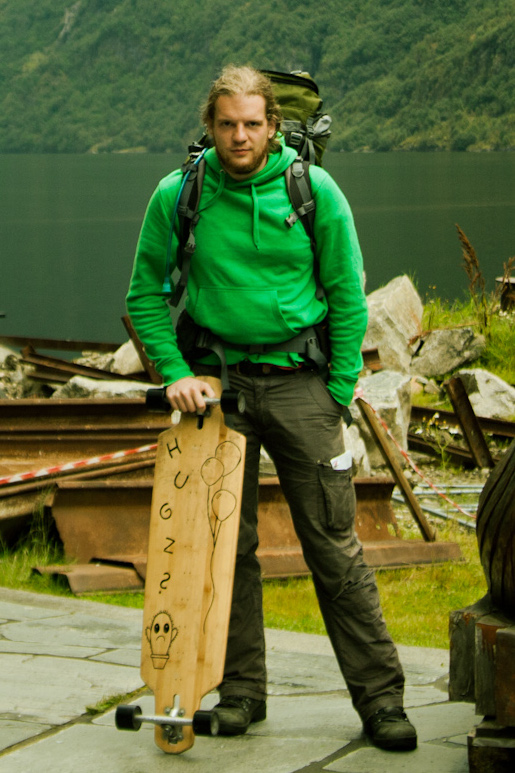
\includegraphics[width=\textwidth]{Fabian}
		\end{column}
		\begin{column}{0.7\textwidth}
			Fabian Pflug\\

			Informatik\\

			5. Master Semester\\

			Android, Genetischer Algorithmus, Webschnittstellen

		\end{column}
	\end{columns}
\end{frame}
\begin{frame}
    \frametitle{Peter Zilz}
	\begin{columns}
		\begin{column}{0.3\textwidth}
			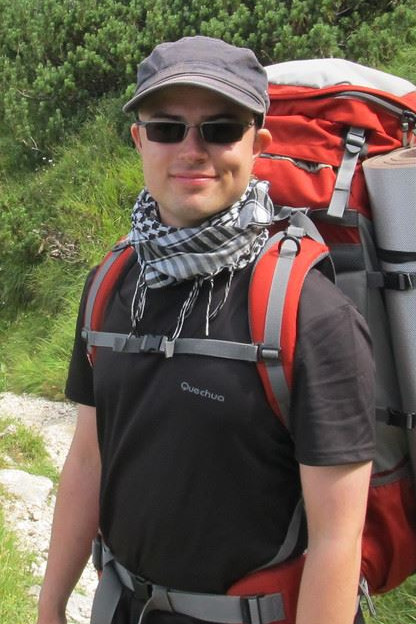
\includegraphics[width=\textwidth]{Peter}
		\end{column}
		\begin{column}{0.7\textwidth}
			Peter Zilz\\

			Mathematiker\\

			5. Master Semester\\

			Visualisierung, Core Componenten, Polygonoperationen

		\end{column}
	\end{columns}
\end{frame}


%%%%%%%%%%%%%%%%%%%%%%%%%%%%%%%%%%%%%%%%%%%%%%%%%%%%%%%%%%%%%%%%%%%%%%%%%%%%%%%%
% oder eine gemeinsame für beide
%%%%%%%%%%%%%%%%%%%%%%%%%%%%%%%%%%%%%%%%%%%%%%%%%%%%%%%%%%%%%%%%%%%%%%%%%%%%%%%%
\begin{frame}
    \frametitle{Über uns}
	\begin{columns}
		\begin{column}{0.25\textwidth}
			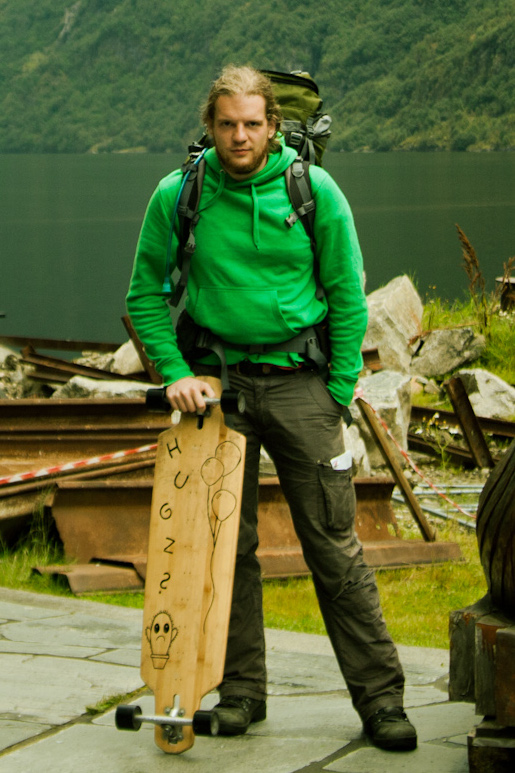
\includegraphics[width=\textwidth]{Fabian}
		\end{column}
		\begin{column}{0.25\textwidth}
		\begin{flushleft}
			Fabian Pflug\\

			Informatik\\

			5. Master Semester\\
		\end{flushleft}
		\end{column}
		\begin{column}{0.25\textwidth}
		\begin{flushright}
			Peter Zilz\\

			Mathematik\\

			5. Master Semester\\
		\end{flushright}
		\end{column}
		\begin{column}{0.25\textwidth}
			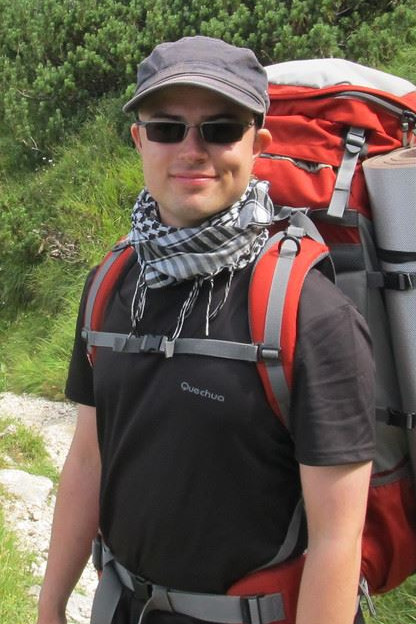
\includegraphics[width=\textwidth]{Peter}
		\end{column}
	\end{columns}
\end{frame}


% die Anfänglichen Sachen

\begin{frame}
    \frametitle{Testdatensatz}
    \begin{center}
    \huge{Probleme}
    \end{center}
\end{frame}

%%%%%%%%%%%%%%%%%%%%%%%%%%%%%%%%%%%%%%%%%%%%%%%%%%%%%%%%%%%%%%%%%%%%%%%%%%%%%%%%
% Bilder noch mal neu machen mit Farbe für Nr. 18 auf Blau!
%%%%%%%%%%%%%%%%%%%%%%%%%%%%%%%%%%%%%%%%%%%%%%%%%%%%%%%%%%%%%%%%%%%%%%%%%%%%%%%%
\begin{frame}
  \frametitle{Inkonsistenz \hfill Lösung Nr. 16}
  \Wider{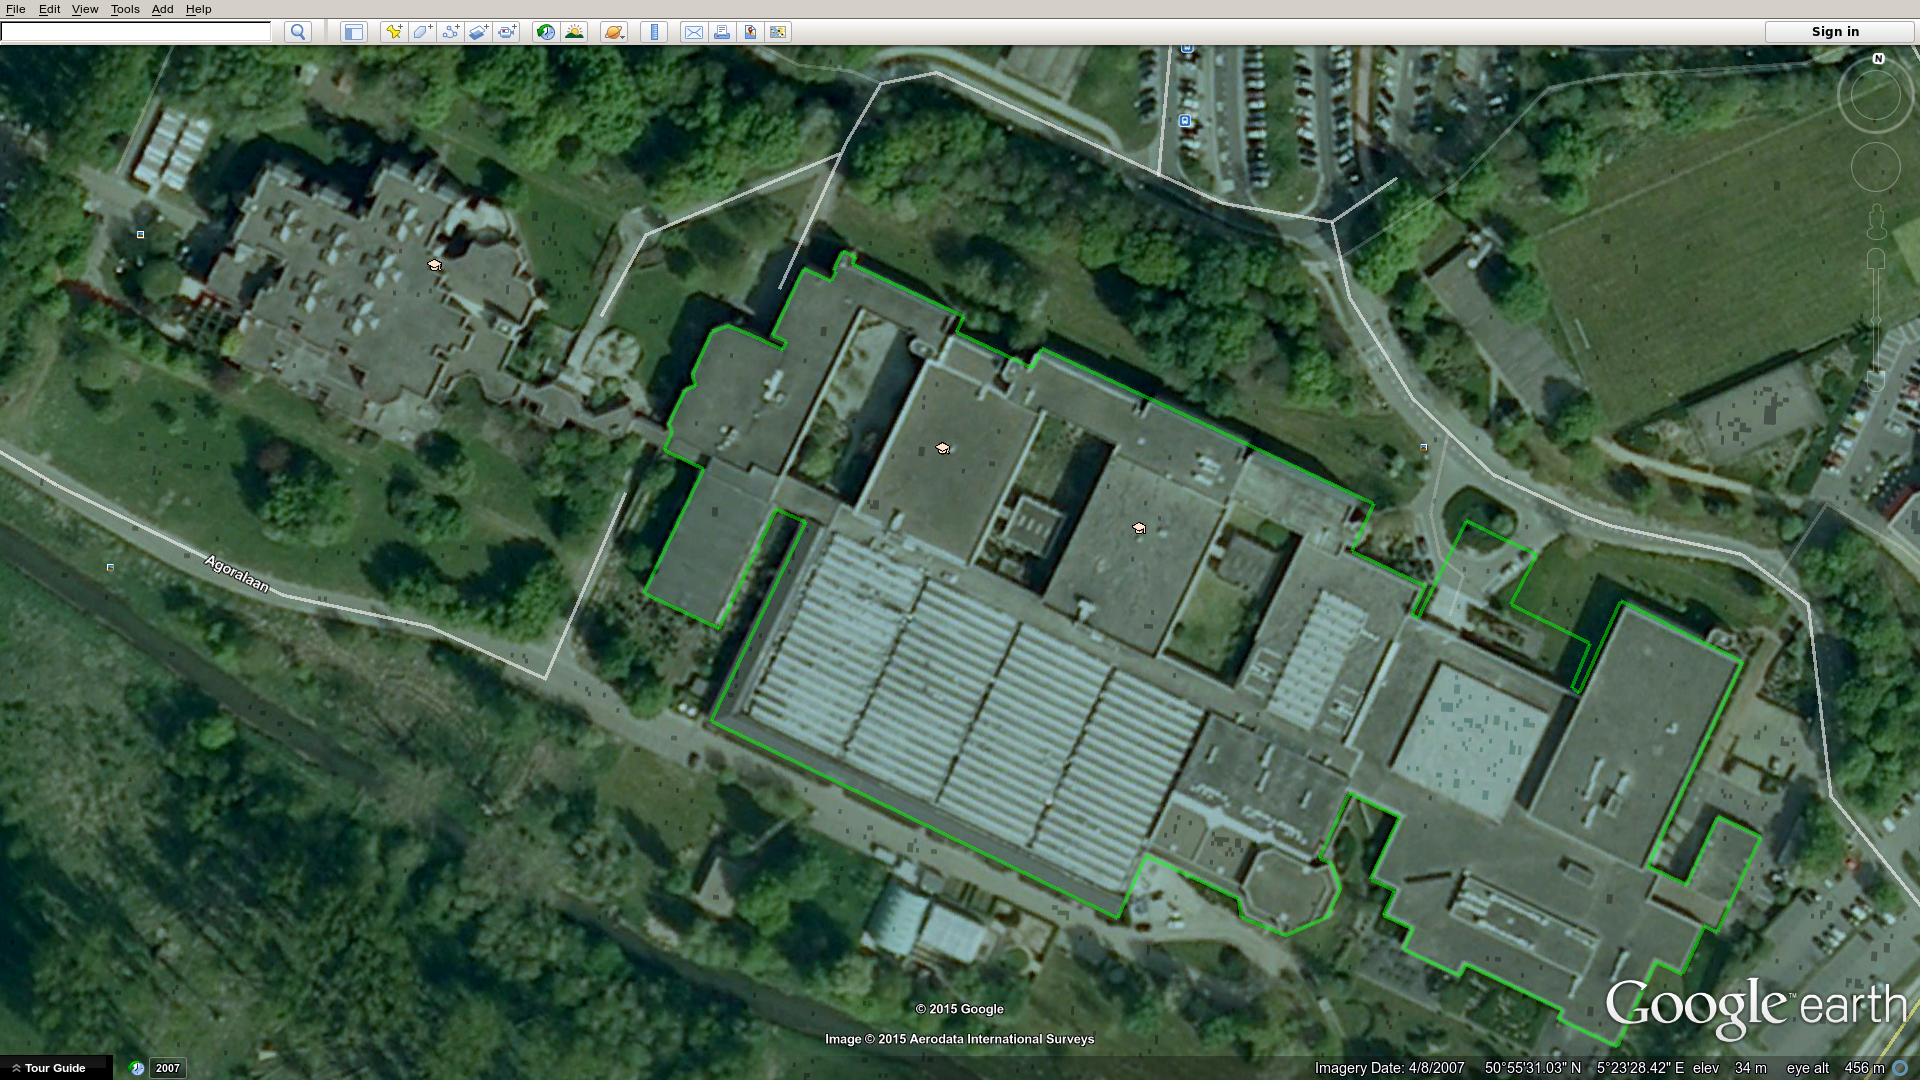
\includegraphics[width=\textwidth]{university_half}}
\end{frame}

\begin{frame}
  \frametitle{Inkonsistenz \hfill Lösung Nr. 18}
  \Wider{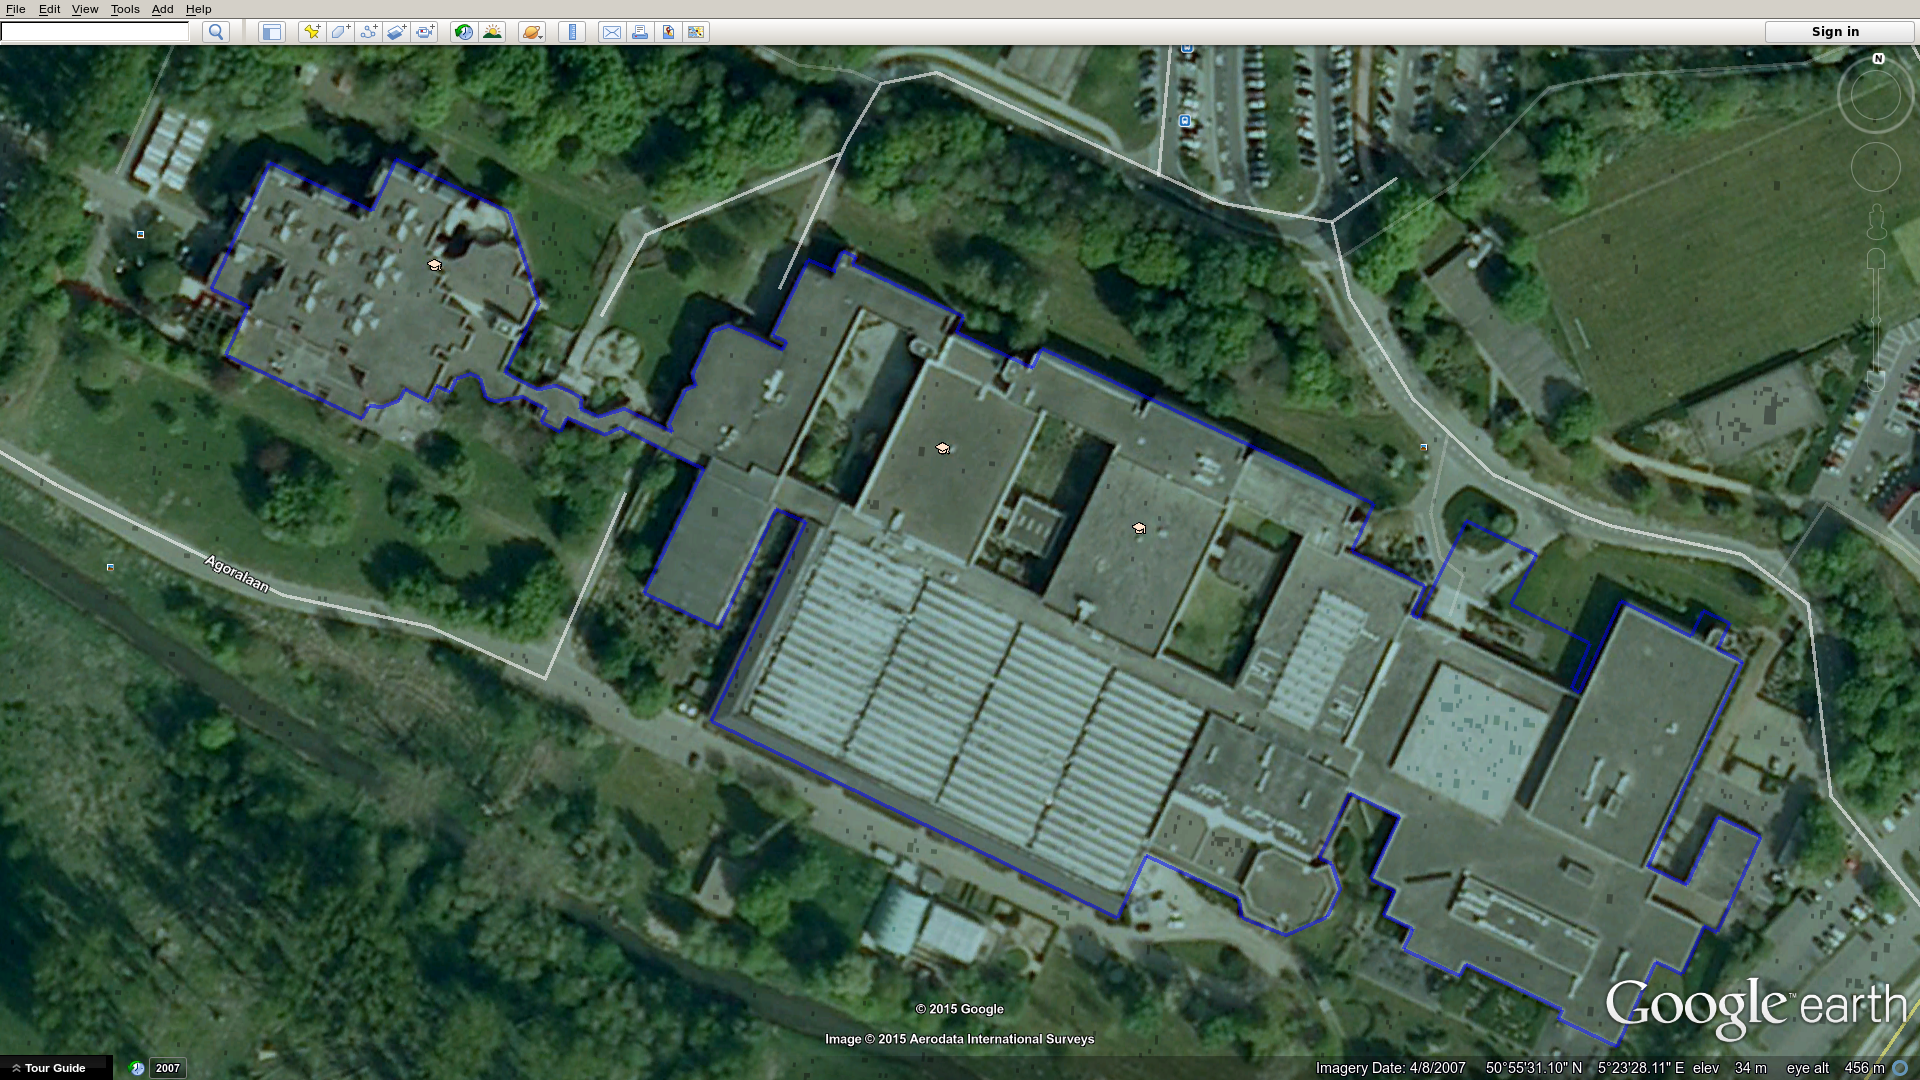
\includegraphics[width=\textwidth]{university_full}}
\end{frame}

\begin{frame}
  \frametitle{Inkonsistenz \hfill Lösung Nr. 16 \& 18}
  \Wider{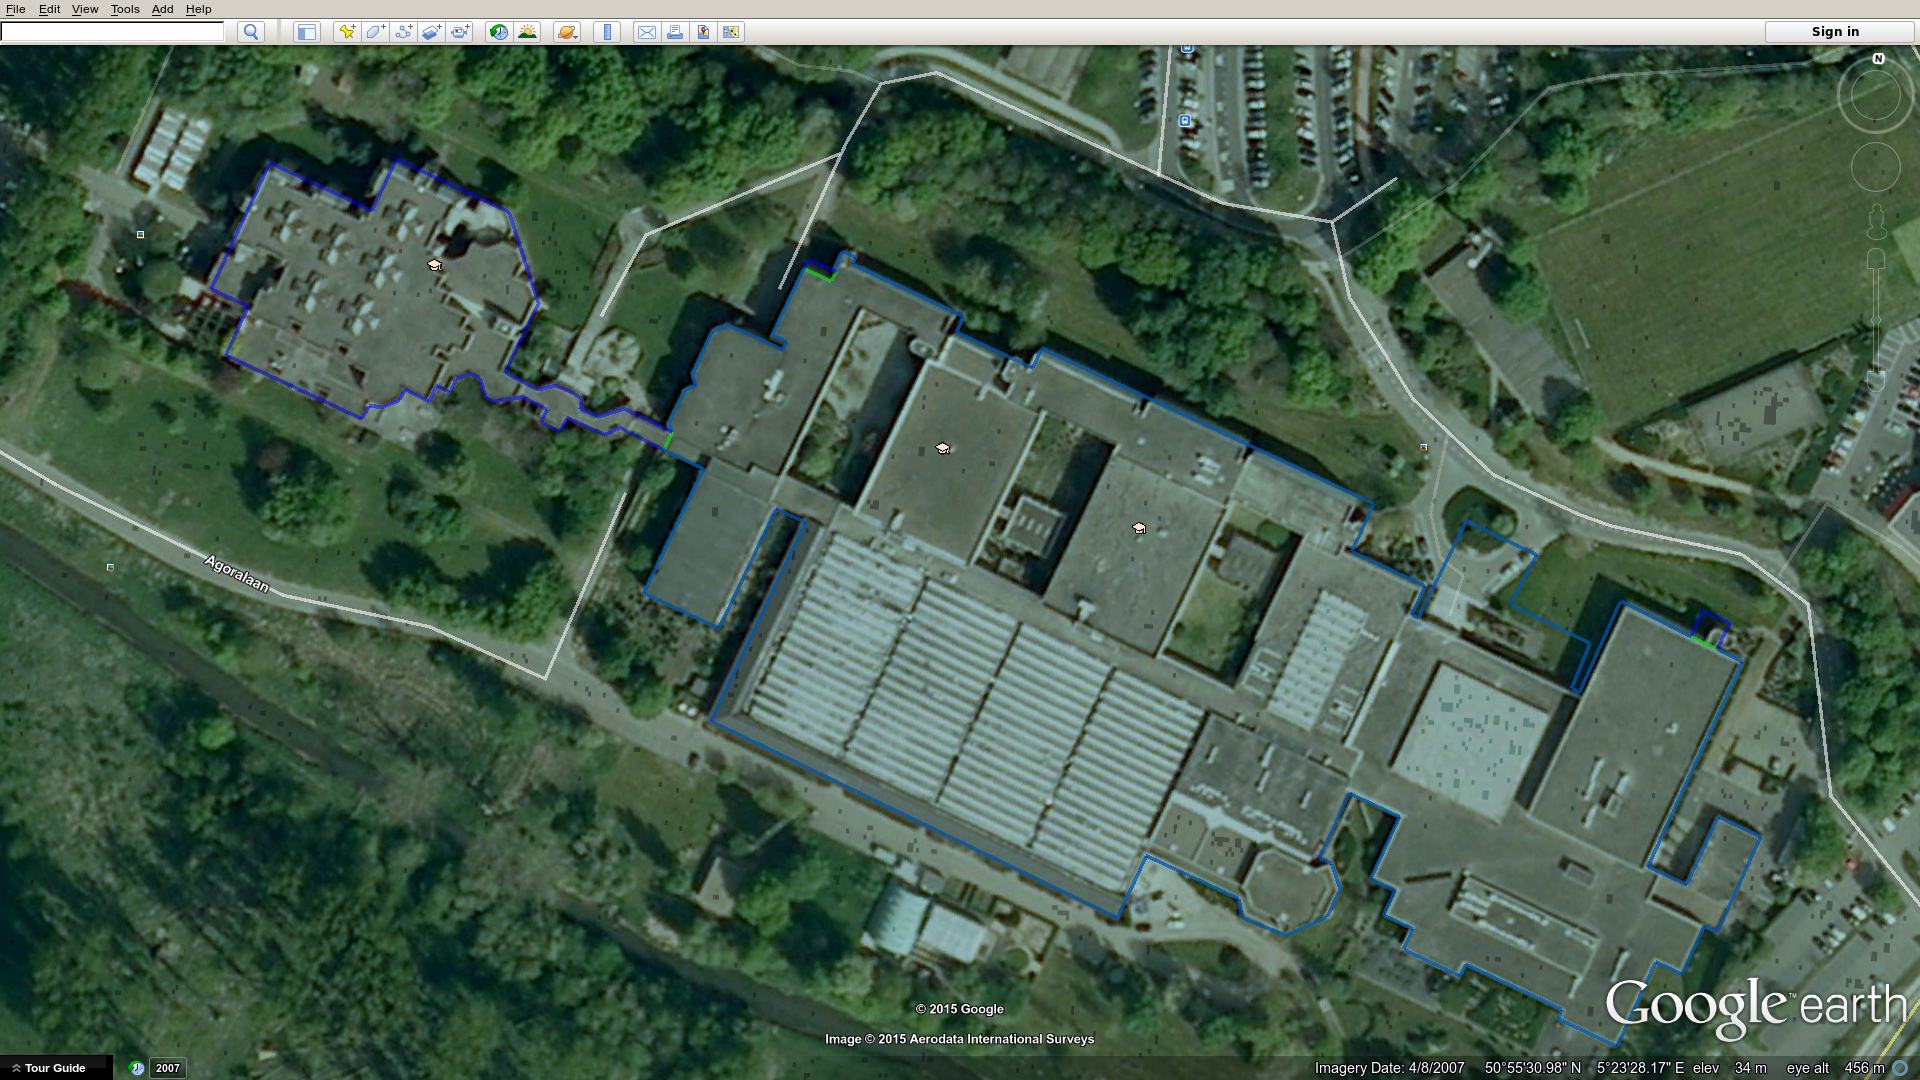
\includegraphics[width=\textwidth]{university_combine}}
\end{frame}

%%%%%%%%%%%%%%%%%%%%%%%%%%%%%%%%%%%%%%%%%%%%%%%%%%%%%%%%%%%%%%%%%%%%%%%%%%%%%%%%
% Bilder noch mal neu machen mit dickerer Strichbreite
%%%%%%%%%%%%%%%%%%%%%%%%%%%%%%%%%%%%%%%%%%%%%%%%%%%%%%%%%%%%%%%%%%%%%%%%%%%%%%%%
\begin{frame}
  \frametitle{Unvollständige Datensätze \hfill Nr. 38}
  \Wider{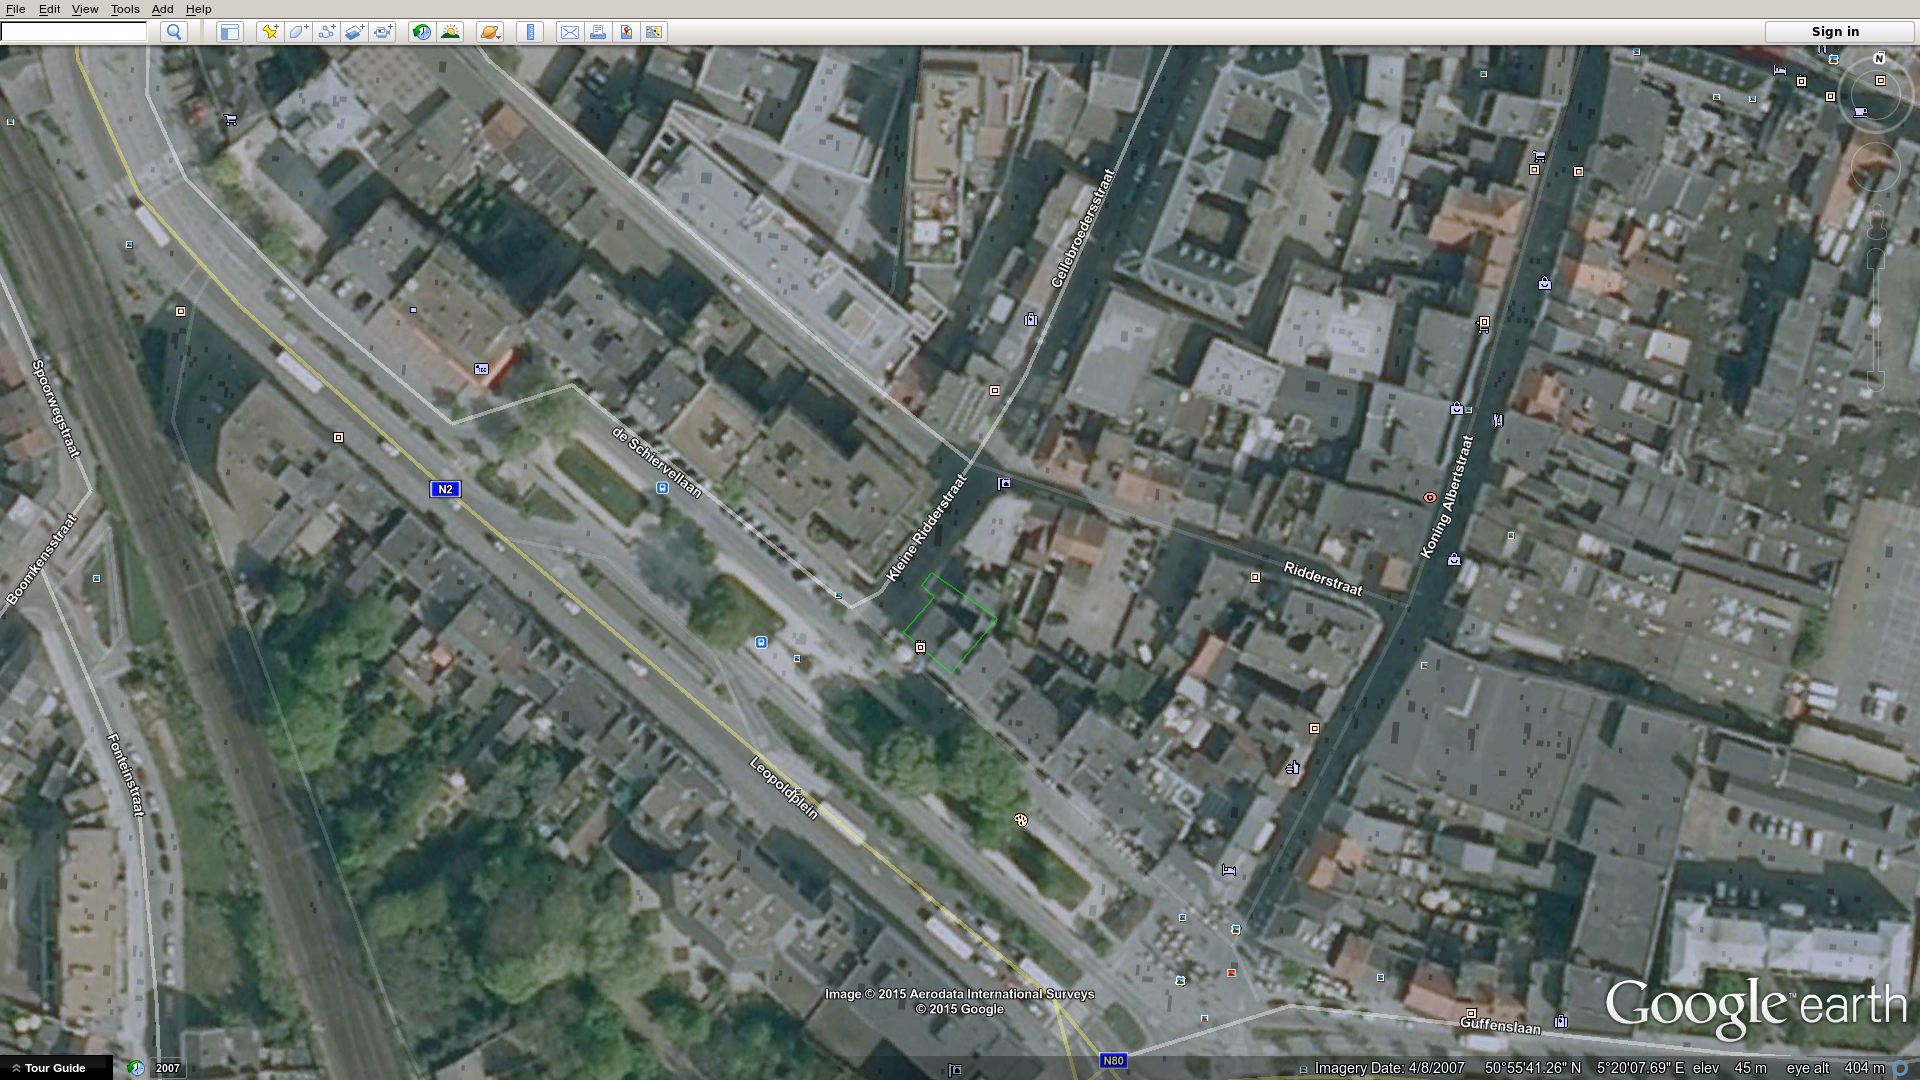
\includegraphics[width=\textwidth]{google_earth}}
\end{frame}

\begin{frame}
  \frametitle{Unvollständige Datensätze \hfill Nr. 38}
  \Wider{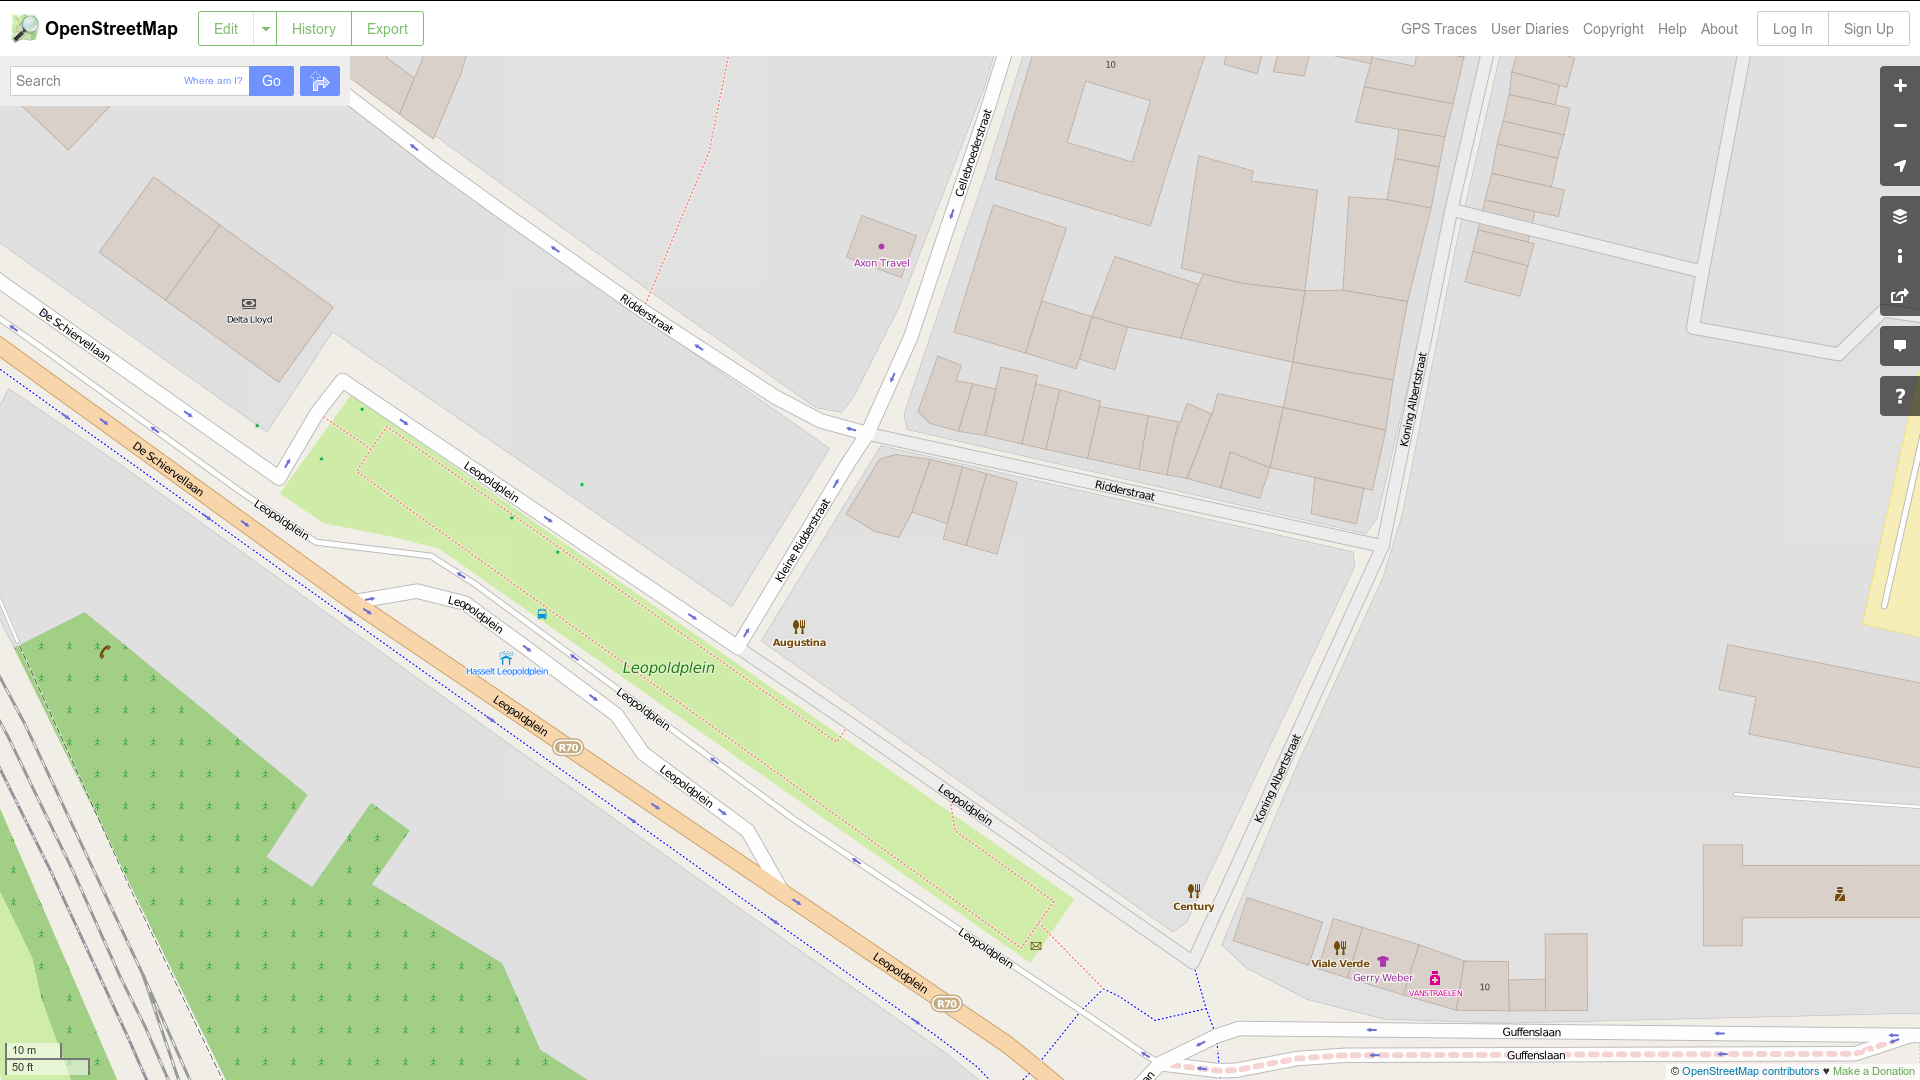
\includegraphics[width=\textwidth]{unvollstaendig}}
\end{frame}


%%%%%%%%%%%%%%%%%%%%%%%%%%%%%%%%%%%%%%%%%%%%%%%%%%%%%%%%%%%%%%%%%%%%%%%%%%%%%%%%
% Auch dickere Strichbreite
%%%%%%%%%%%%%%%%%%%%%%%%%%%%%%%%%%%%%%%%%%%%%%%%%%%%%%%%%%%%%%%%%%%%%%%%%%%%%%%%
\begin{frame}
  \frametitle{Falsche Datensätze \hfill Nr. 40}
  \Wider{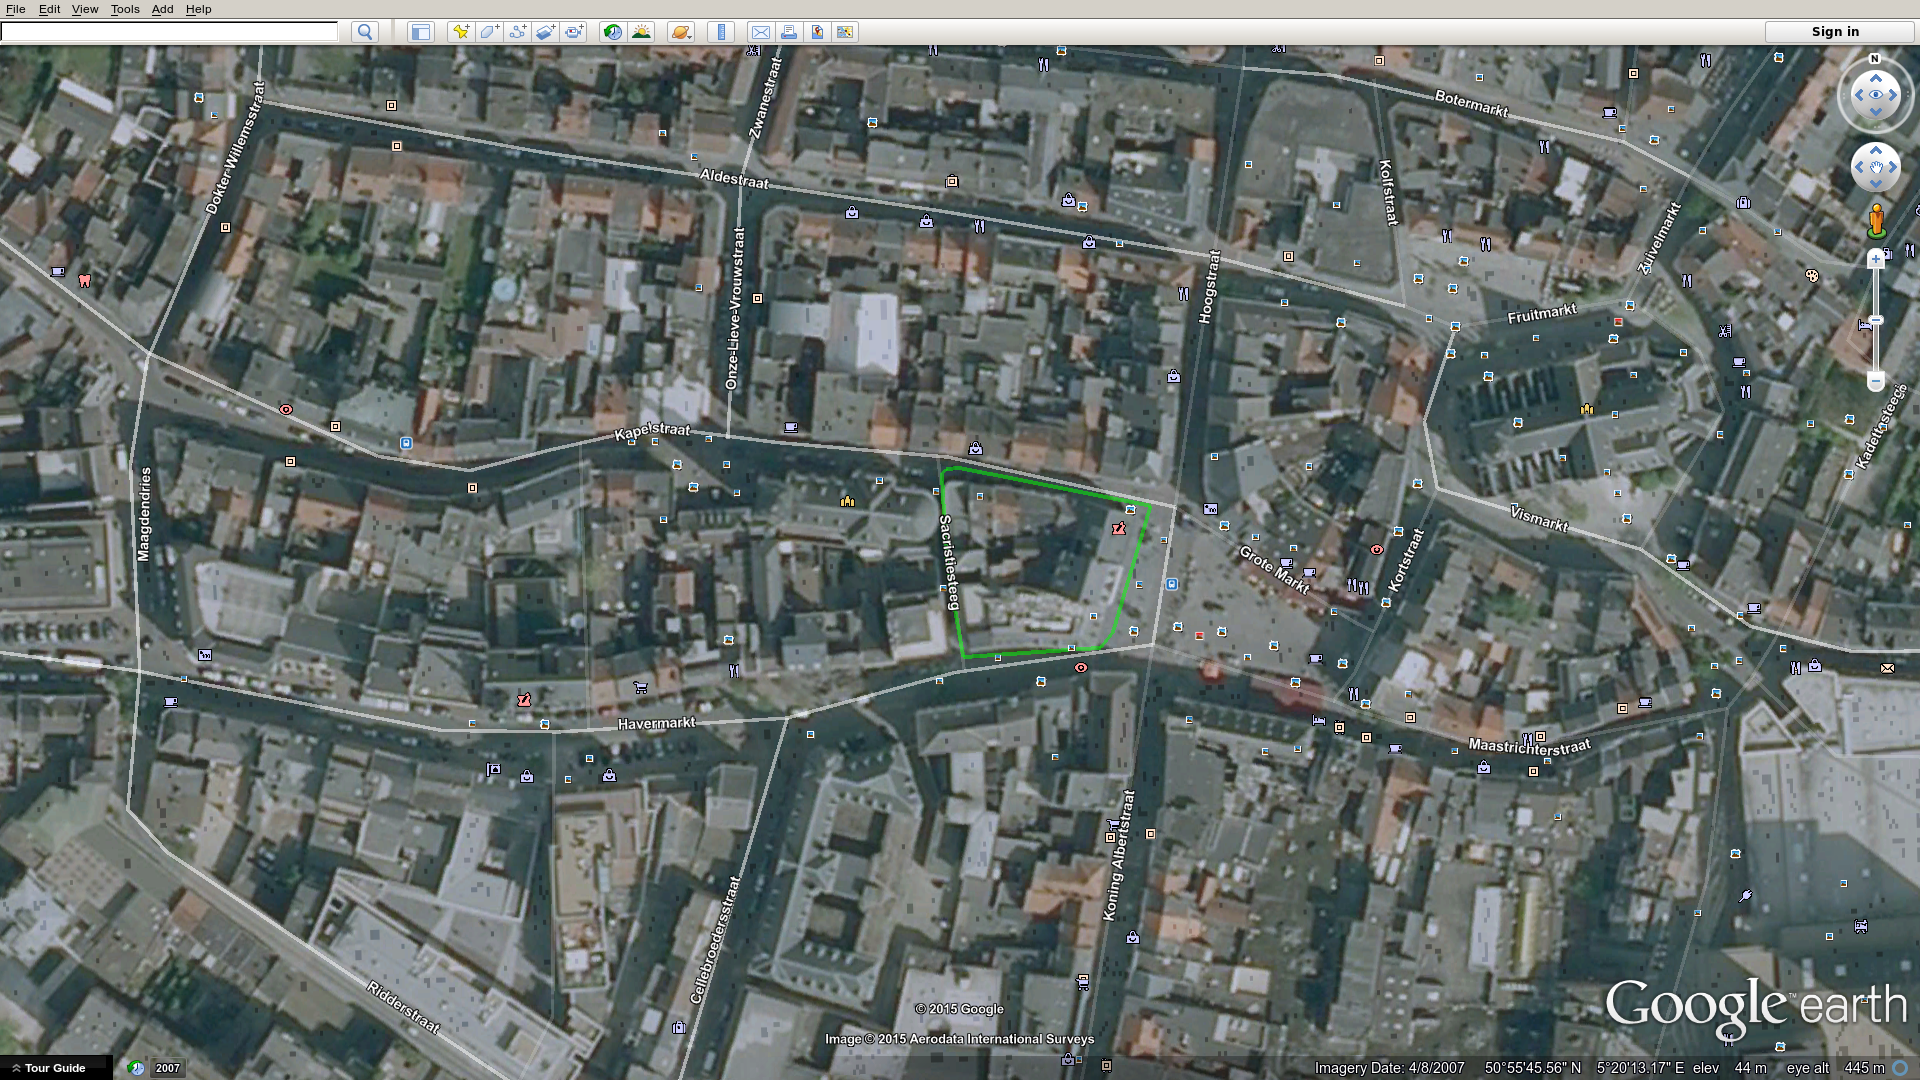
\includegraphics[width=\textwidth]{40_fail_earth}}
\end{frame}

\begin{frame}
  \frametitle{Falsche Datensätze \hfill Nr. 40}
  \Wider{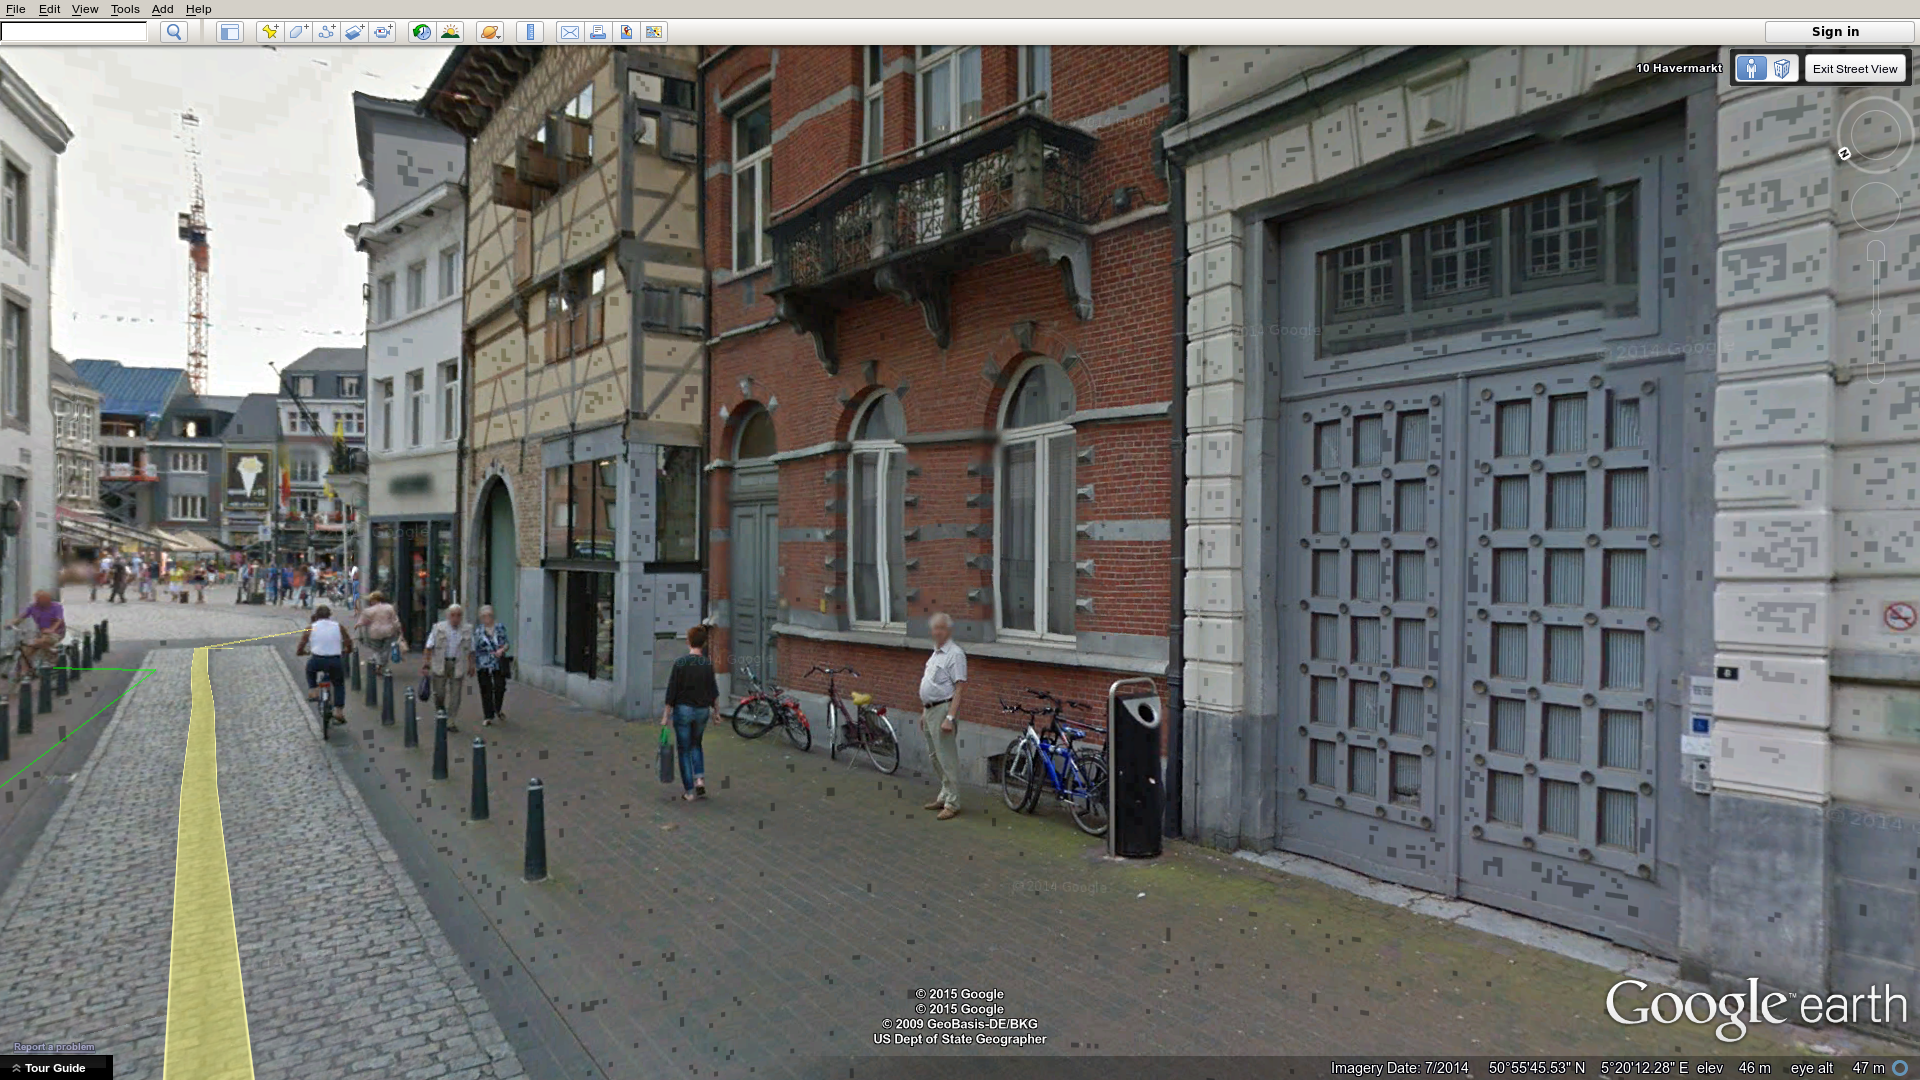
\includegraphics[width=\textwidth]{40_fail_street}}
\end{frame}

\begin{frame}
  \frametitle{Falsche Datensätze \hfill Nr. 40}
  \Wider{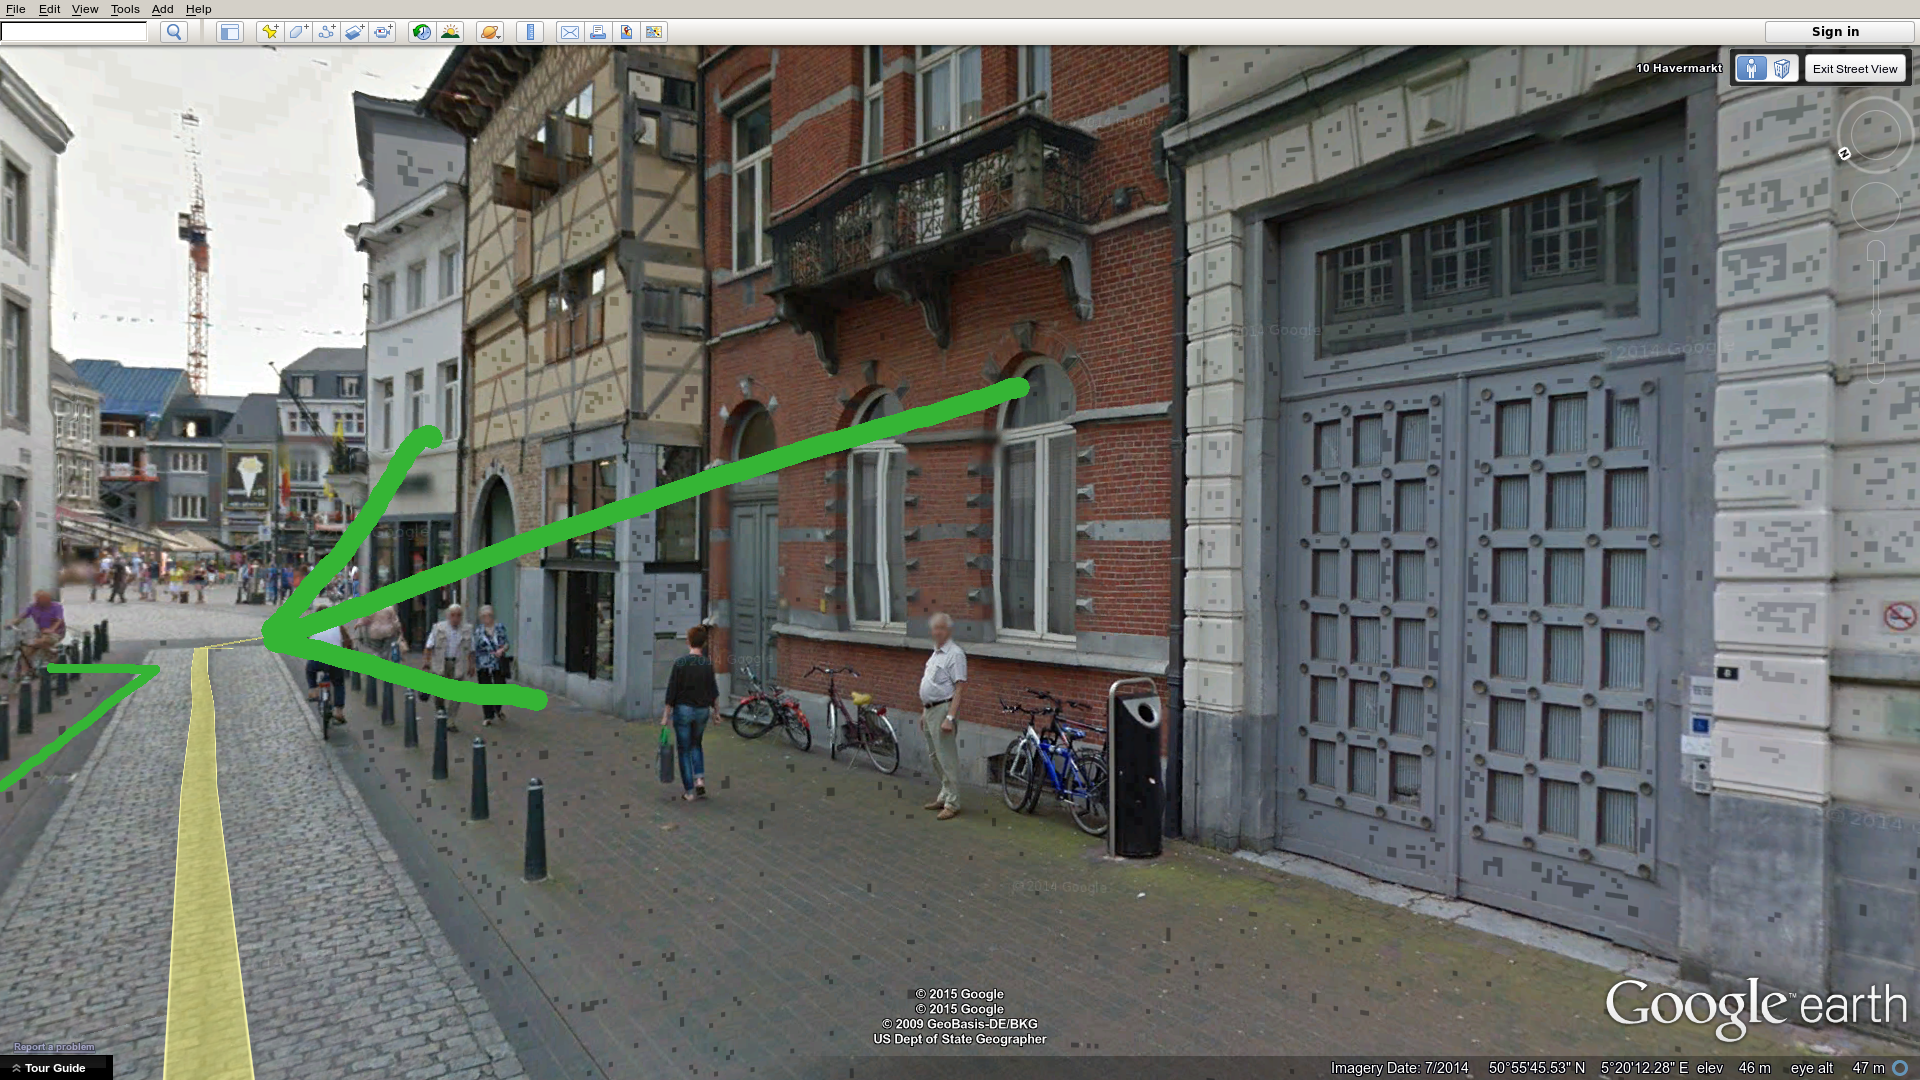
\includegraphics[width=\textwidth]{40_fail_street_building}}
\end{frame}

\begin{frame}
  \frametitle{Falsche Datensätze \hfill Nr. 40}
  \Wider{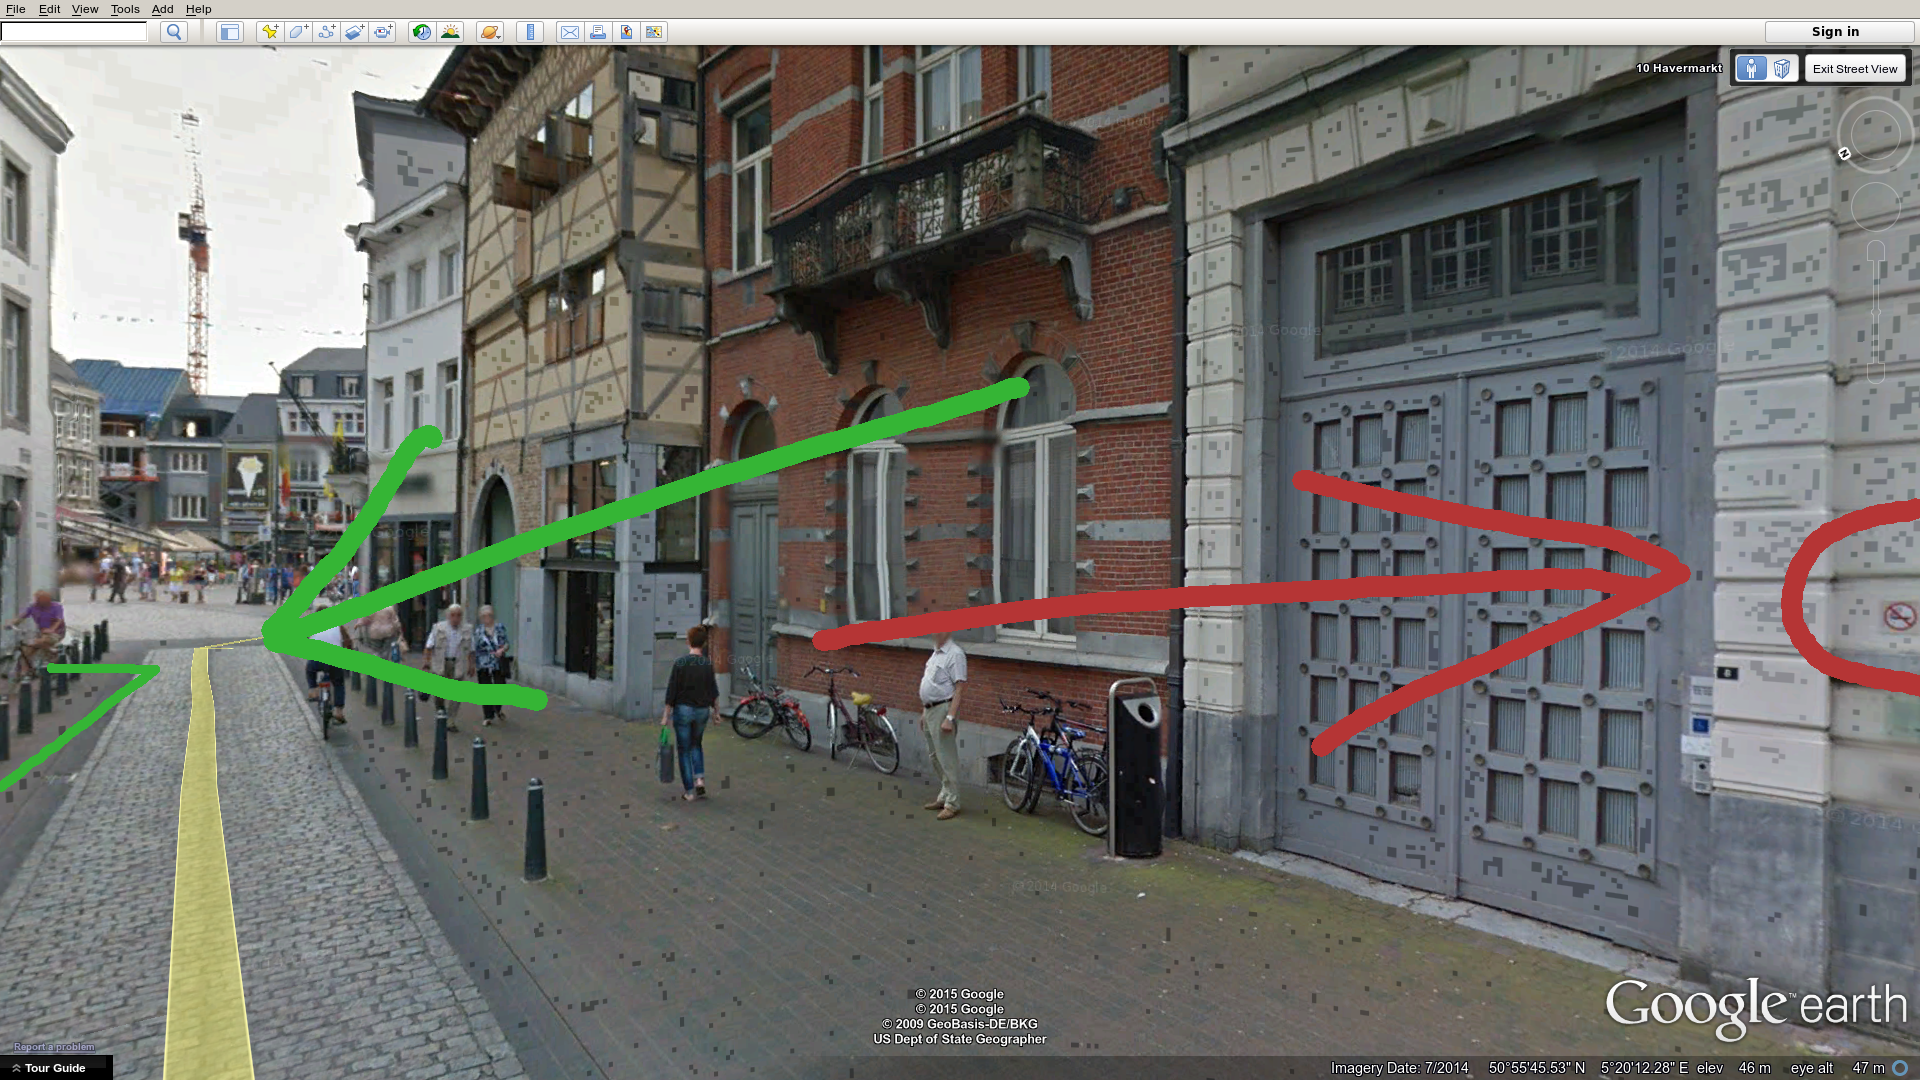
\includegraphics[width=\textwidth]{40_fail_street_sign}}
\end{frame}

%\begin{frame}
%  \frametitle{Falsche Datensätze \hfill Nr. 40}
%  \Wider{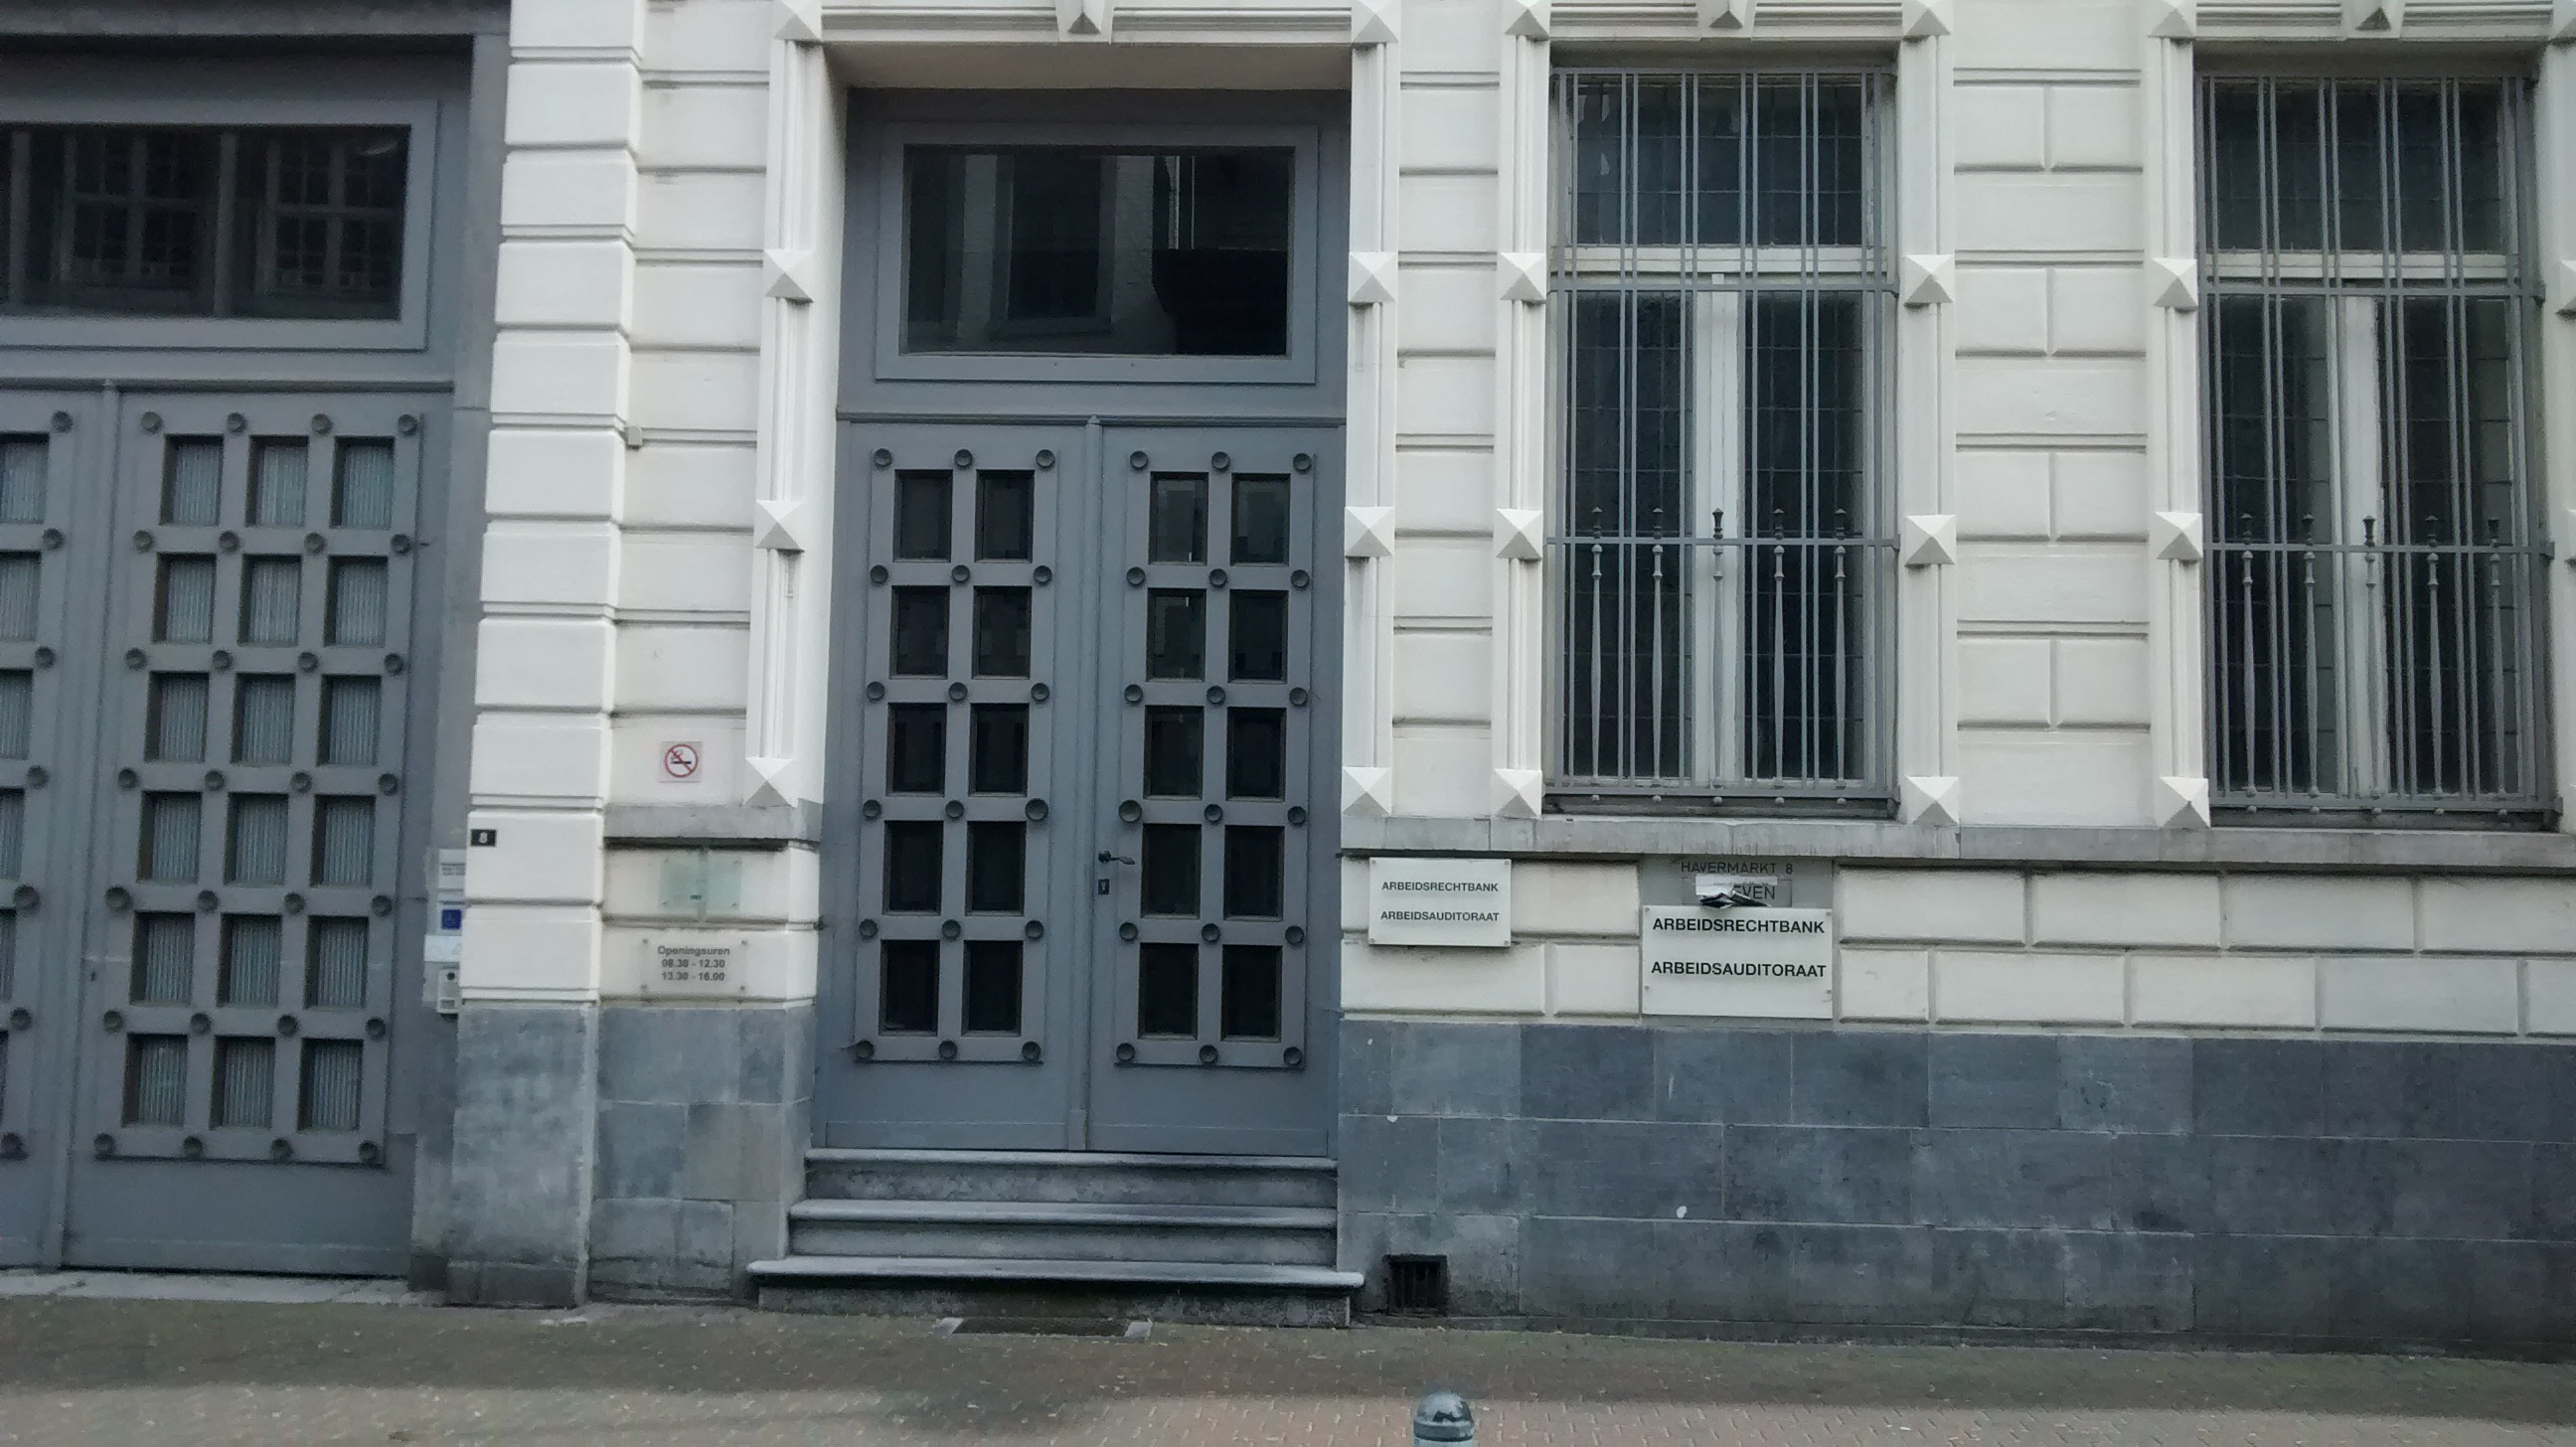
\includegraphics[width=\textwidth]{0040}}
%\end{frame}


%%%%%%%%%%%%%%%%%%%%%%%%%%%%%%%%%%%%%%%%%%%%%%%%%%%%%%%%%%%%%%%%%%%%%%%%%%%%%%%%
% Formatierung von dem hier verbessern!
%%%%%%%%%%%%%%%%%%%%%%%%%%%%%%%%%%%%%%%%%%%%%%%%%%%%%%%%%%%%%%%%%%%%%%%%%%%%%%%%
\begin{frame}
  \frametitle{3 Klassen}
\begin{columns}
  \begin{column}{0.33\textwidth}
  Einfache Datensätze
  \begin{itemize}
  \item 1 - 15
  \item 17 - 32
  \item 35
  \item 37
  \item 42
  \item 46 - 48
  \item 52
  \item 54
  \item 63 - 83
  \item 86 - 89
  \item 91 - 92
  \item 94 - 95
  \end{itemize}
  \end{column}
    \begin{column}{0.33\textwidth}
    Unvollständige Datensätze
    \begin{itemize}
    \item 33 - 34
    \item 36
    \item 38
    \item 39
    \item 41
    \item 43 - 45
    \item 49 - 50
    \item 55 - 62
    \end{itemize}
    \end{column}
  \begin{column}{0.33\textwidth}
  Schwere Datensätze
  \begin{itemize}
  \item 16
  \item 33
  \item 40
  \item 43
  \item 51
  \item 57
  \item 59
  \item 62
  \item 84
  \item 85
  \item 90
  \item 93
  \item 96
  \end{itemize}
  \end{column}
\end{columns}
\end{frame}


% Wie es zu unserem algorithmus gekommen ist
\begin{frame}
  \frametitle{Visualisierung}
  \Wider{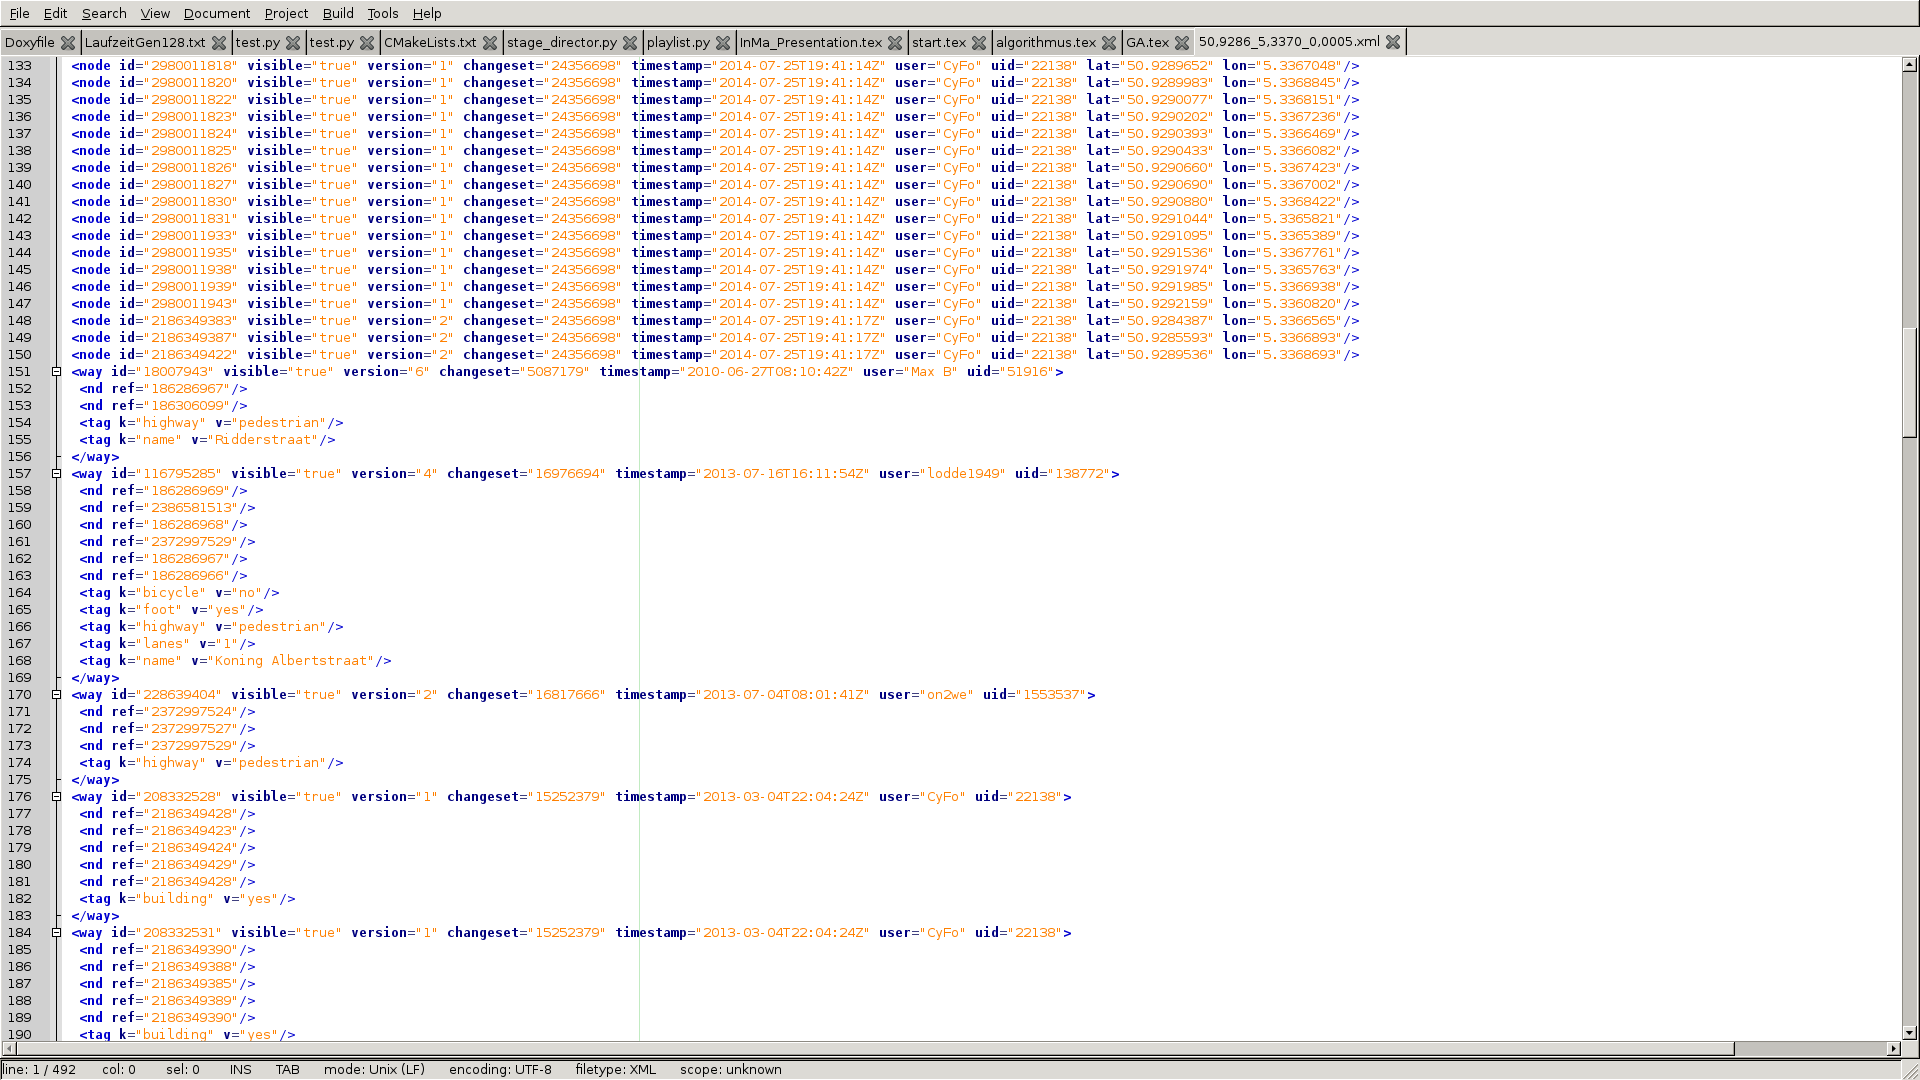
\includegraphics[width=\textwidth]{XML}}
\end{frame}

\begin{frame}
  \frametitle{Visualisierung}
%%%%%%%%%%%%%%%%%%%%%%%%%%%%%%%%%%%%%%%%%%%%%%%%%%%%%%%%%%%%%%%%%%%%%%%%%%%%%%%%
  % Hier ein Bild von unserer Visualisierungsklasse
  % danach ein Frame mit Bild, bei dem die Tags von einem Teil vergrößert sind (Picture in Picture)
  % danach ein Frame mit Bild, bei dem zusätzlich noch die richtige Lösung und unser Tipp farbig eingezeichnet sind
  % vielleicht hier dann erst mal unsere Idee darstellen.
  % danach ein Frame mit Bild, bei dem gezeigt wird, dass die Tags jetzt noch zusätlich "entfernung" und "gewichtete Entfernung"
%%%%%%%%%%%%%%%%%%%%%%%%%%%%%%%%%%%%%%%%%%%%%%%%%%%%%%%%%%%%%%%%%%%%%%%%%%%%%%%%
\end{frame}

\begin{frame}
  \frametitle{Coverage}
  \begin{equation*}
    Coverage = \frac{Area_{intersection}}{max(Area_{guesspolygon},Area_{loesungspolygon})}
  \end{equation*}
\\
  \begin{equation*}
    Coverage \in {0..1}
  \end{equation*}
%%%%%%%%%%%%%%%%%%%%%%%%%%%%%%%%%%%%%%%%%%%%%%%%%%%%%%%%%%%%%%%%%%%%%%%%%%%%%%%%
% Vielleicht hier 3 kleine Beispiele für Coverage.
% 0: intersection = null
% 1: intersection = lösung  % oder beliebige andere
% 0.1: Lösung ist 1/10 von guess groß und liegt in ihr drinne
%%%%%%%%%%%%%%%%%%%%%%%%%%%%%%%%%%%%%%%%%%%%%%%%%%%%%%%%%%%%%%%%%%%%%%%%%%%%%%%%
\end{frame}

\begin{frame}
  \frametitle{Naiver Ansatz}
%%%%%%%%%%%%%%%%%%%%%%%%%%%%%%%%%%%%%%%%%%%%%%%%%%%%%%%%%%%%%%%%%%%%%%%%%%%%%%%%
% Coverage Wert für den Naiven Ansatz Einfügen
%%%%%%%%%%%%%%%%%%%%%%%%%%%%%%%%%%%%%%%%%%%%%%%%%%%%%%%%%%%%%%%%%%%%%%%%%%%%%%%%
  \begin{center}
  \huge{Coverage = ...}
  \end{center}
\end{frame}

\begin{frame}
  \frametitle{Gewichteter Ansatz}
%%%%%%%%%%%%%%%%%%%%%%%%%%%%%%%%%%%%%%%%%%%%%%%%%%%%%%%%%%%%%%%%%%%%%%%%%%%%%%%%
% Coverage Wert für den Naiven und ersten Ansatz Einfügen
%%%%%%%%%%%%%%%%%%%%%%%%%%%%%%%%%%%%%%%%%%%%%%%%%%%%%%%%%%%%%%%%%%%%%%%%%%%%%%%%
  \begin{center}
  \huge{Coverage = ...}
  \end{center}
  \begin{center}
  Naive Coverage = ...
  \end{center}
\end{frame}

\begin{frame}
  \frametitle{Unvollständige Daten}
%%%%%%%%%%%%%%%%%%%%%%%%%%%%%%%%%%%%%%%%%%%%%%%%%%%%%%%%%%%%%%%%%%%%%%%%%%%%%%%%
% Bild von unserer Image-Klasse mit einem unvollständigen Datensatz (am besten wieder 38)
%%%%%%%%%%%%%%%%%%%%%%%%%%%%%%%%%%%%%%%%%%%%%%%%%%%%%%%%%%%%%%%%%%%%%%%%%%%%%%%%
\end{frame}

\begin{frame}
  \frametitle{Umgebungspolygon}
%%%%%%%%%%%%%%%%%%%%%%%%%%%%%%%%%%%%%%%%%%%%%%%%%%%%%%%%%%%%%%%%%%%%%%%%%%%%%%%%
% Erklärung zu dem Umkreispolygon und dem anschließenden schneiden.
%%%%%%%%%%%%%%%%%%%%%%%%%%%%%%%%%%%%%%%%%%%%%%%%%%%%%%%%%%%%%%%%%%%%%%%%%%%%%%%%
\end{frame}

\begin{frame}
  \frametitle{Umgebungspolygon}
%%%%%%%%%%%%%%%%%%%%%%%%%%%%%%%%%%%%%%%%%%%%%%%%%%%%%%%%%%%%%%%%%%%%%%%%%%%%%%%%
% Bild von unserer Image-Klasse mit einem unvollständigen Datensatz und dem geschnittenen Ansatz (am besten wieder 38)
%%%%%%%%%%%%%%%%%%%%%%%%%%%%%%%%%%%%%%%%%%%%%%%%%%%%%%%%%%%%%%%%%%%%%%%%%%%%%%%%
\end{frame}

\begin{frame}
  \frametitle{Vollständiger Ansatz}
%%%%%%%%%%%%%%%%%%%%%%%%%%%%%%%%%%%%%%%%%%%%%%%%%%%%%%%%%%%%%%%%%%%%%%%%%%%%%%%%
% Coverage Wert für den vollständigen und ersten Ansatz Einfügen
%%%%%%%%%%%%%%%%%%%%%%%%%%%%%%%%%%%%%%%%%%%%%%%%%%%%%%%%%%%%%%%%%%%%%%%%%%%%%%%%
  \begin{center}
  \huge{Coverage = ...}
  \end{center}
  \begin{center}
  Vorheriger Coverage = ...
  \end{center}
\end{frame}

\begin{frame}
  \frametitle{Sonstige Verbesserungen}
  \begin{itemize}
    \item Partielle Gebäude zu einem zusammen gefügt
    \item OSM-Daten zwischengespeichert
    \item GPS-Daten aus Bildern auslesen.
%%%%%%%%%%%%%%%%%%%%%%%%%%%%%%%%%%%%%%%%%%%%%%%%%%%%%%%%%%%%%%%%%%%%%%%%%%%%%%%%
% Weitere Verbesserungen die wir gemacht haben, aber nicht groß erklären wollen.
%%%%%%%%%%%%%%%%%%%%%%%%%%%%%%%%%%%%%%%%%%%%%%%%%%%%%%%%%%%%%%%%%%%%%%%%%%%%%%%%
    \item ...
  \end{itemize}
\end{frame}

\begin{frame}
    \frametitle{rules.xml Format}
    %Content goes here
\end{frame}


% Was wir danach noch gemacht haben mit GA und Android
\begin{frame}
    \frametitle{Genetischer Algorithmus}
    \begin{itemize}
      \item<1-> unendlich viele Möglichkeiten
      \item<2-> Lösung sind bekannt.
      \item<2-> Trainingsdaten vorhanden
      \item<3-> Später einfacher Regeln zu erstellen.
    \end{itemize}
\end{frame}

\begin{frame}
  \frametitle{Coverage}
  \begin{center}
  \huge{GA Coverage = 73,1 \%}
  \end{center}
  \begin{center}
  \huge{Human Coverage = 74,6 \%}
  \end{center}
\end{frame}


\begin{frame}
    \frametitle{App um mehr Daten zu bekommen}
    \begin{itemize}
      \item<1-> Hoffnung auf mehr Testdaten
      \item<2-> Direkter Nutzen für beteiligte Personen
      \item<3-> Nie über alpha-stadium hinaus gekommen
      \item<4-> Open Source, also fühlt euch frei.
    \end{itemize}
\end{frame}

\begin{frame}
  \frametitle{Startbildschirm}
  \Wider{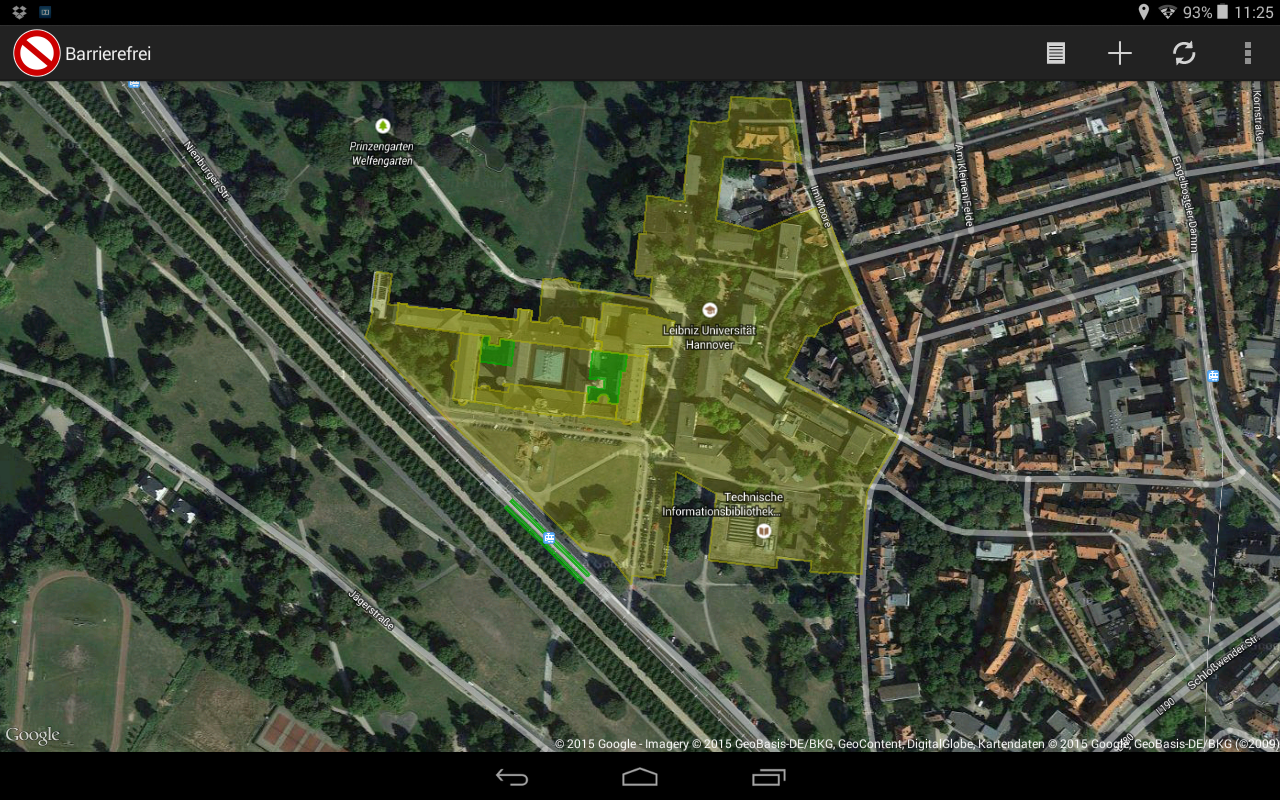
\includegraphics[width=\textwidth]{App_show}}
\end{frame}

\begin{frame}
  \frametitle{Tags}
  \Wider{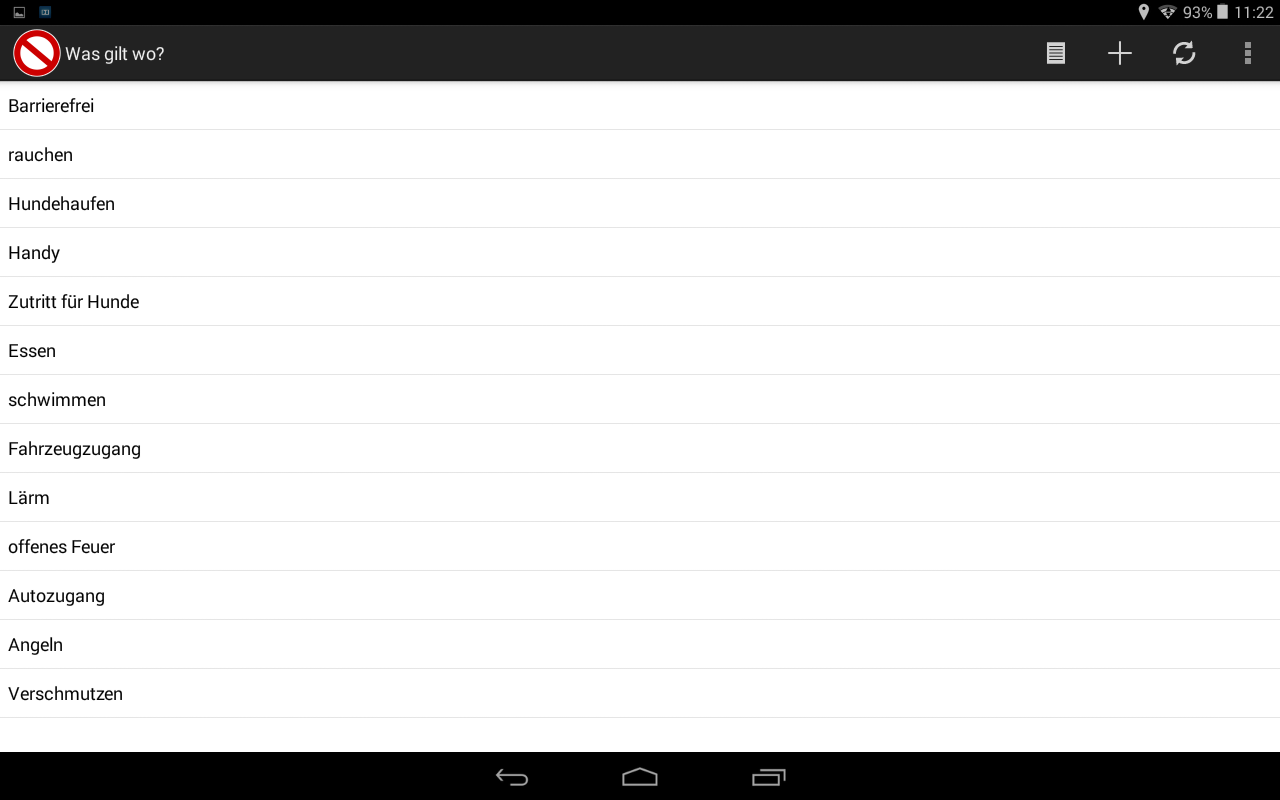
\includegraphics[width=\textwidth]{App_tags}}
\end{frame}

\begin{frame}
  \frametitle{Fläche auswählen}
  \Wider{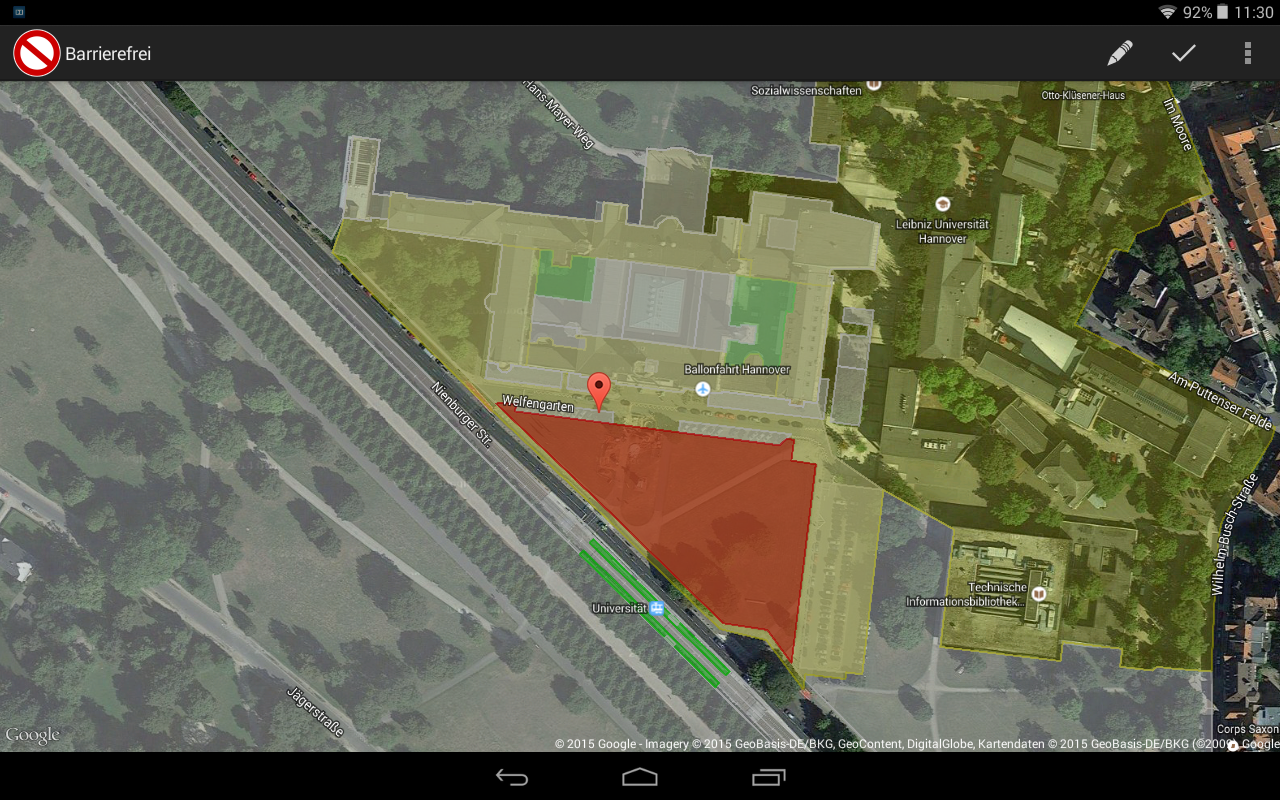
\includegraphics[width=\textwidth]{App_select}}
\end{frame}

\begin{frame}
  \frametitle{Frei einzeichnen}
  \Wider{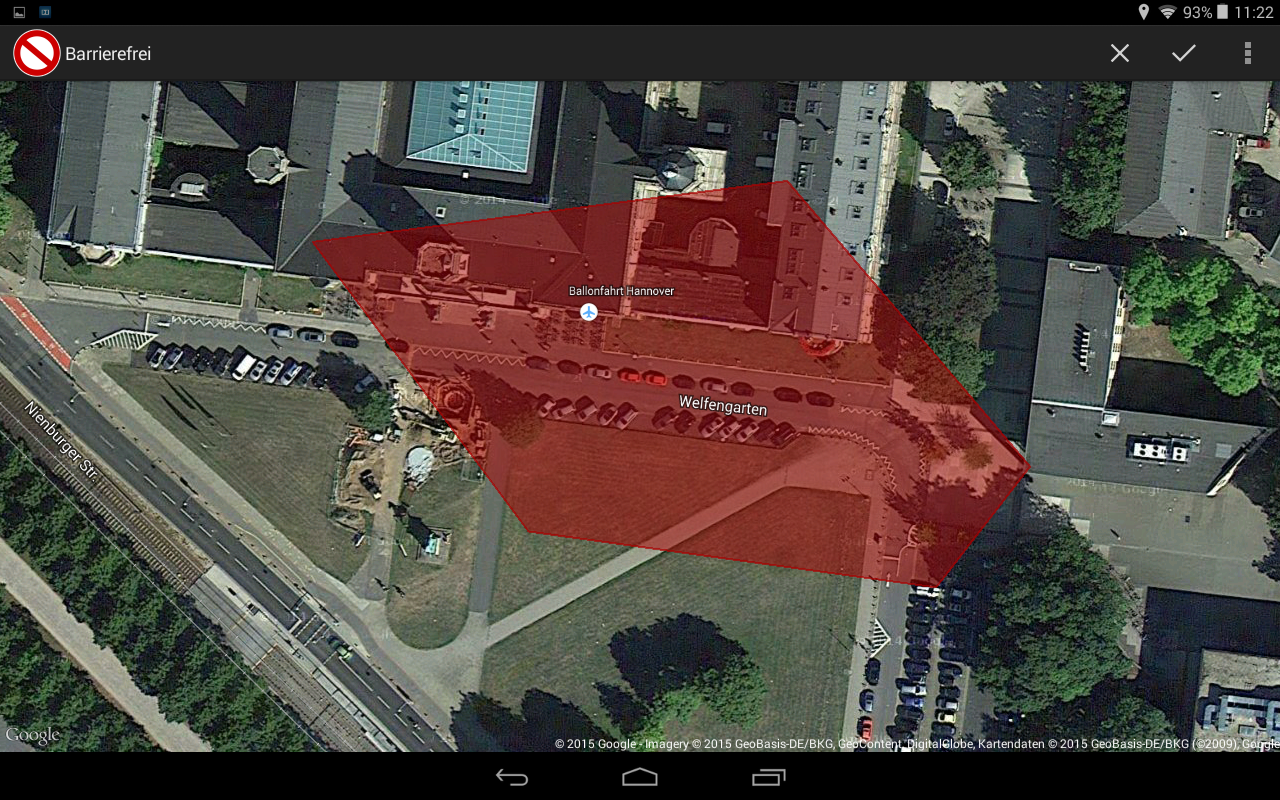
\includegraphics[width=\textwidth]{App_free}}
\end{frame}


\begin{frame}
    \frametitle{Bibliotheken}
    \begin{itemize}
      \item jts (http://www.vividsolutions.com/jts/JTSHome.htm)
      \item jsoup (http://jsoup.org/)
      \item LaTeX
      \item Git / GitHub
    \end{itemize}
\end{frame}

\begin{frame}
    \frametitle{Ende}
    \begin{center}
    \huge{Fragen?}
    \end{center}
\end{frame}

% alles was wir nach dem ende noch an Extrafolien haben wollen.
%%%%%%%%%%%%%%%%%%%%%%%%%%%%%%%%%%%%%%%%%%%%%%%%%%%%%%%%%%%%%%%%%%%%%%%%%%%%%%%%
% Es könnten Fragen kommen, warum nur 70%
% hier dann Bilder von der Uni und allen anderen Gebäuden, die wir nicht haben mappen können.
%%%%%%%%%%%%%%%%%%%%%%%%%%%%%%%%%%%%%%%%%%%%%%%%%%%%%%%%%%%%%%%%%%%%%%%%%%%%%%%%
\begin{frame}[fragile]
  \frametitle{rules.xml Format}
  \lstset{language=XML,basicstyle=\scriptsize}
  \lstinputlisting{Rules.xml}
\end{frame}


\begin{frame}
 \frametitle{70\%}
    \begin{itemize}
	\item 10 * University
	\item Verschiebungen in OSM zu real (3, 7)
	\item umkreis ist nie perfekt
    \end{itemize}
\end{frame}

\begin{frame}
 \frametitle{Nicht geschafft}
  \Wider{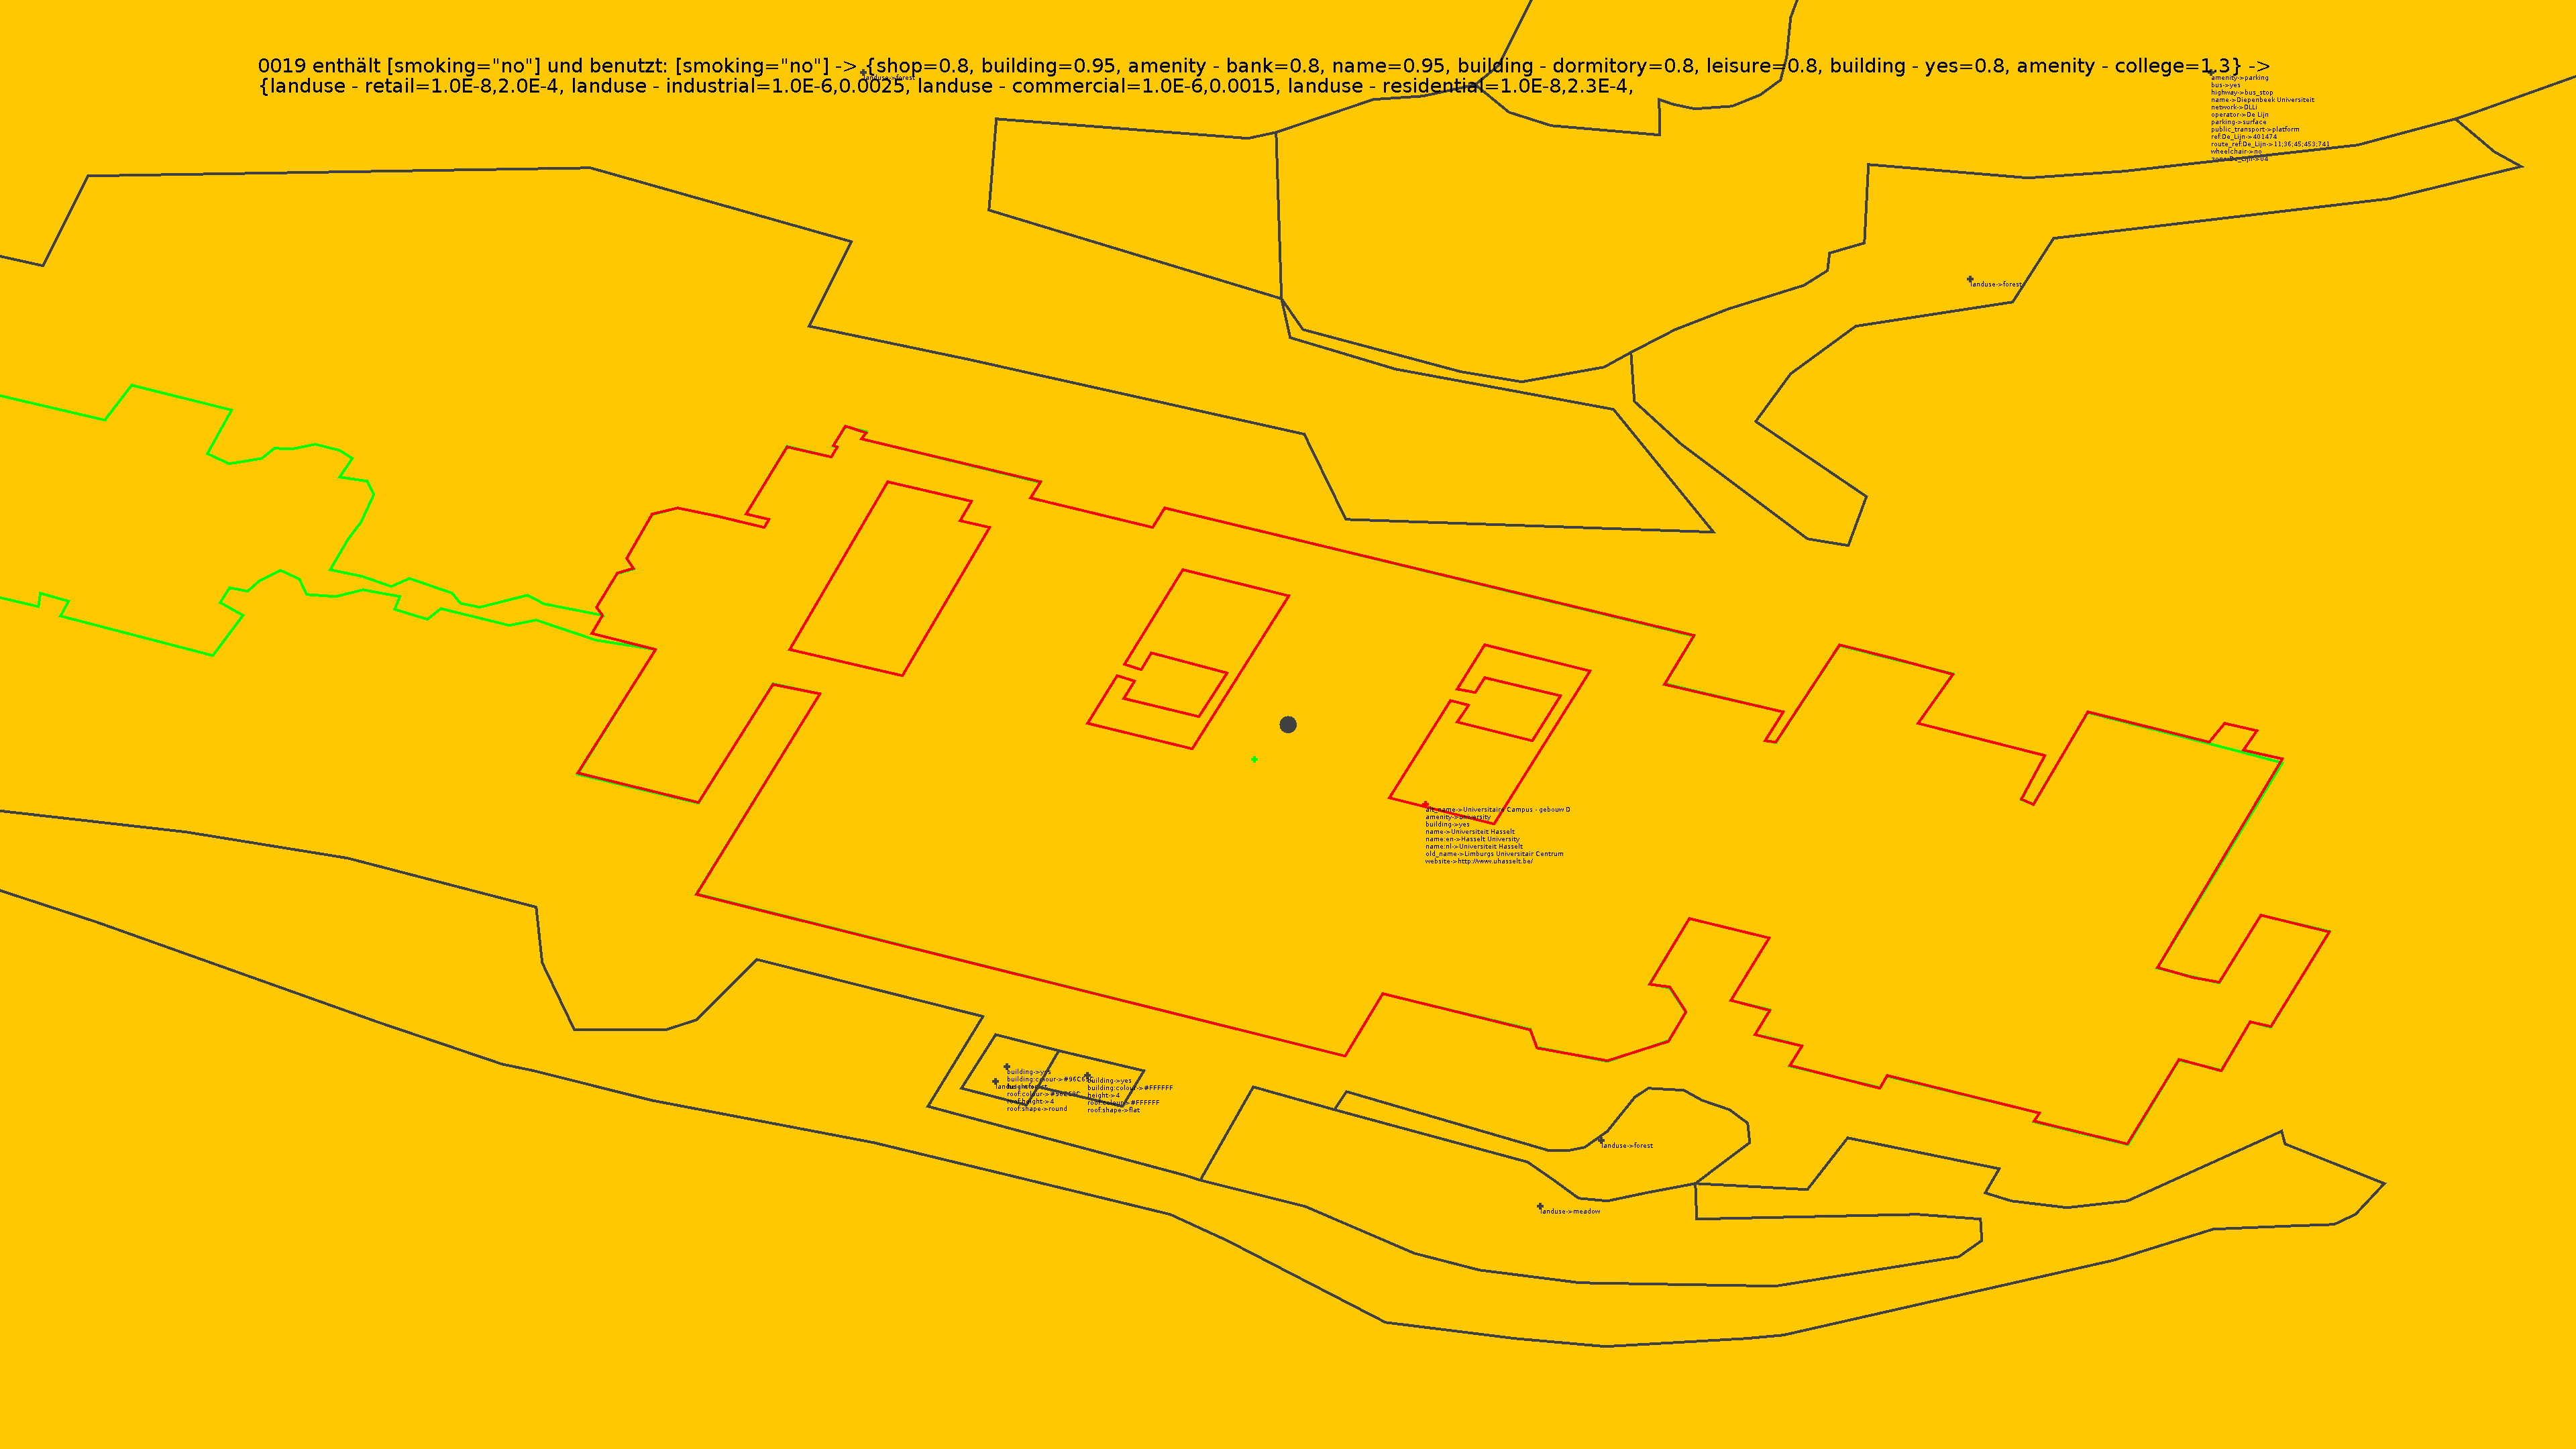
\includegraphics[width=\textwidth]{0019_big.png}}
\end{frame}


\begin{frame}
 \frametitle{Nicht geschafft}
  \Wider{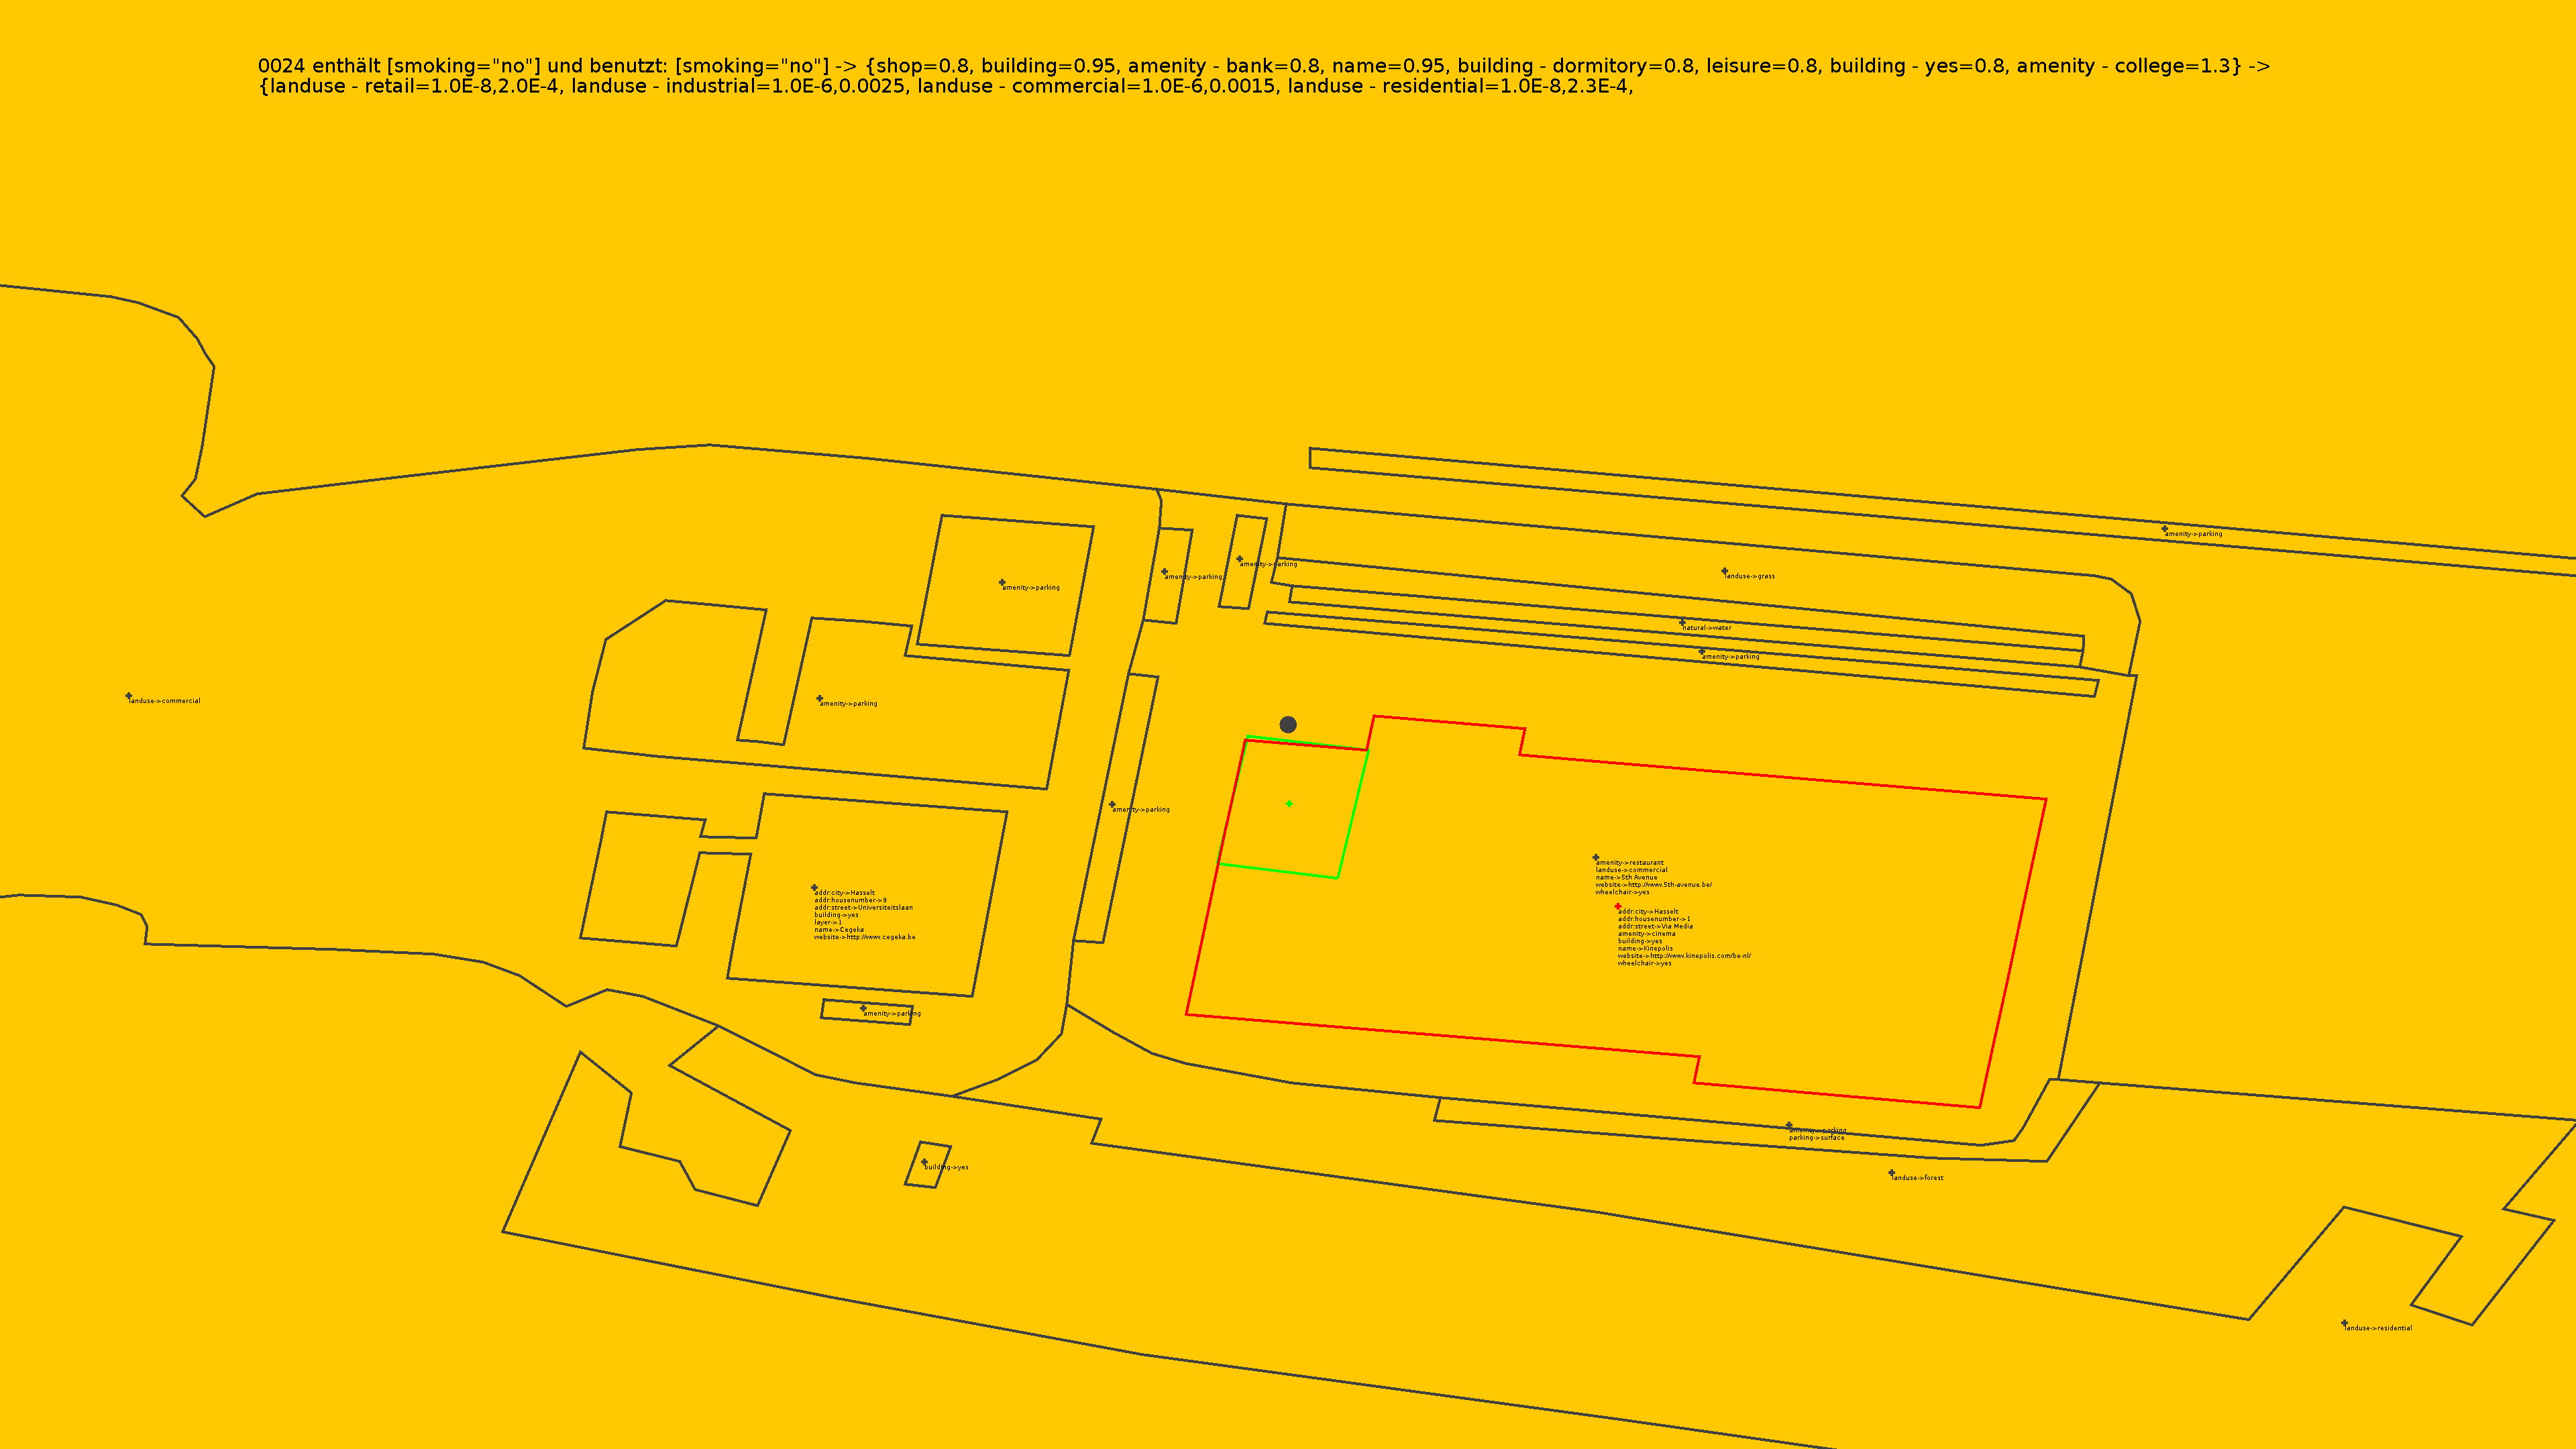
\includegraphics[width=\textwidth]{0024_big.png}}
\end{frame}


\begin{frame}
 \frametitle{Nicht geschafft}
  \Wider{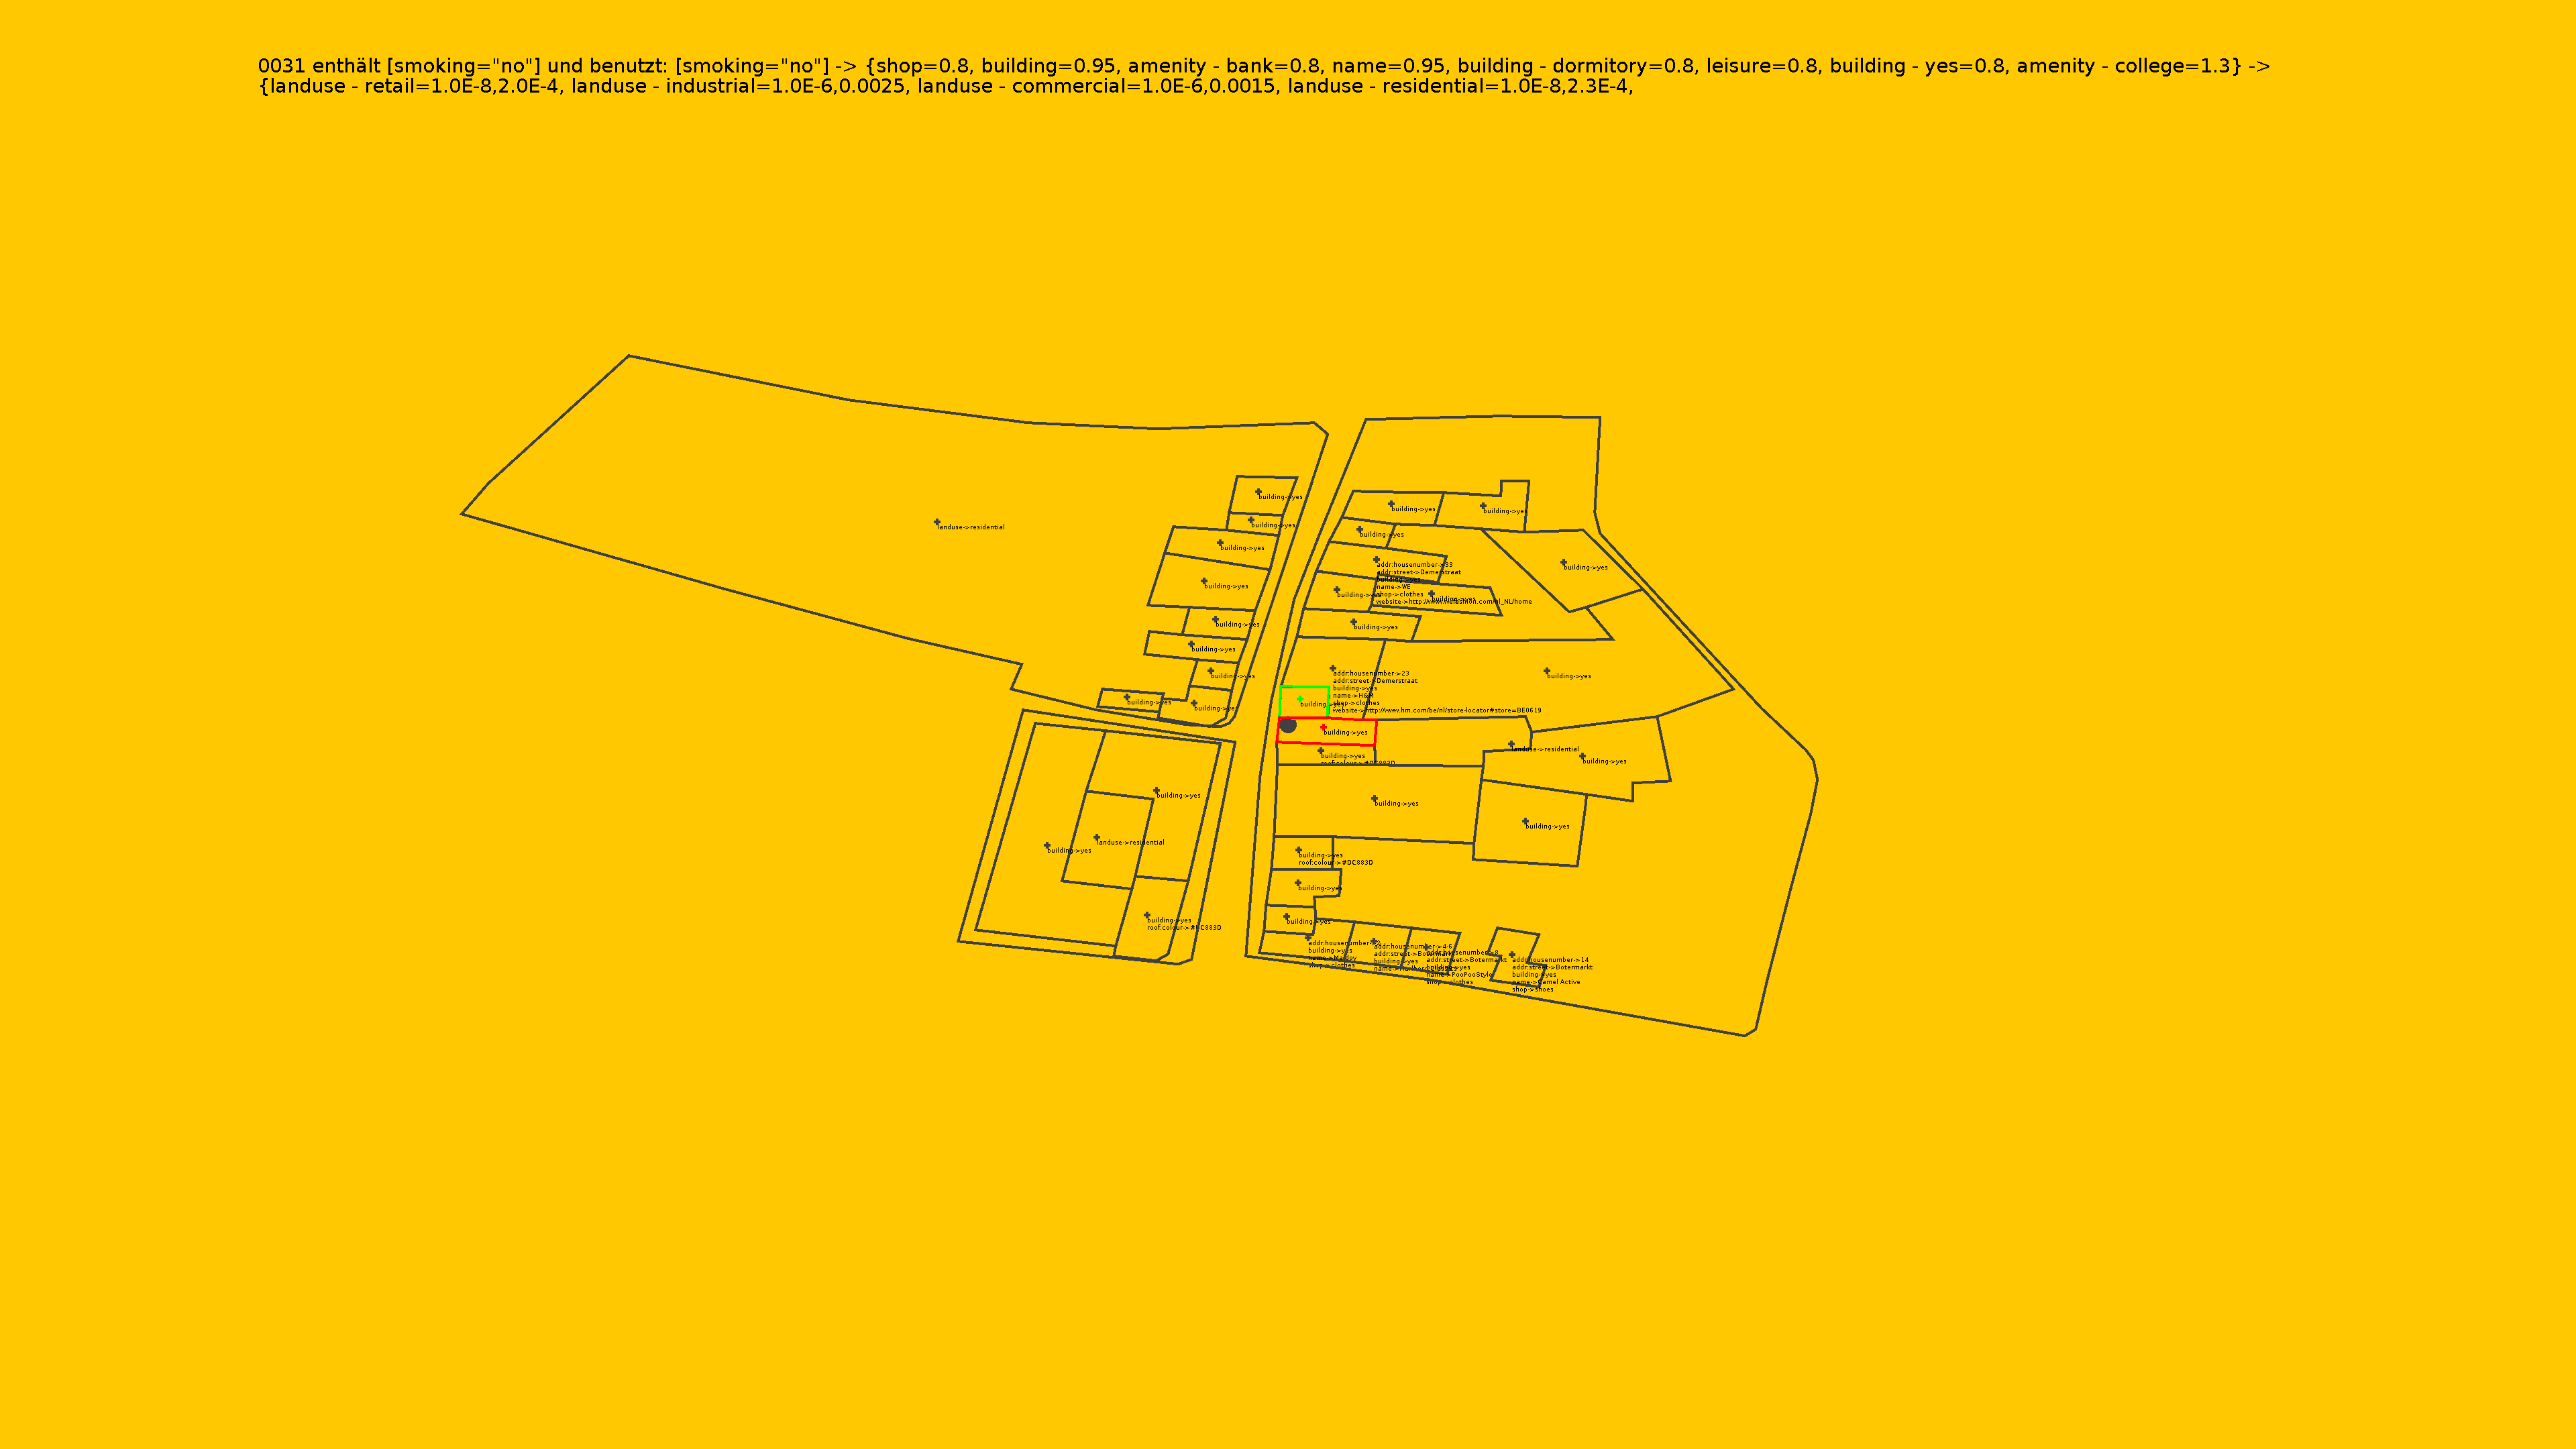
\includegraphics[width=\textwidth]{0031_big.png}}
\end{frame}


\begin{frame}
 \frametitle{Nicht geschafft}
  \Wider{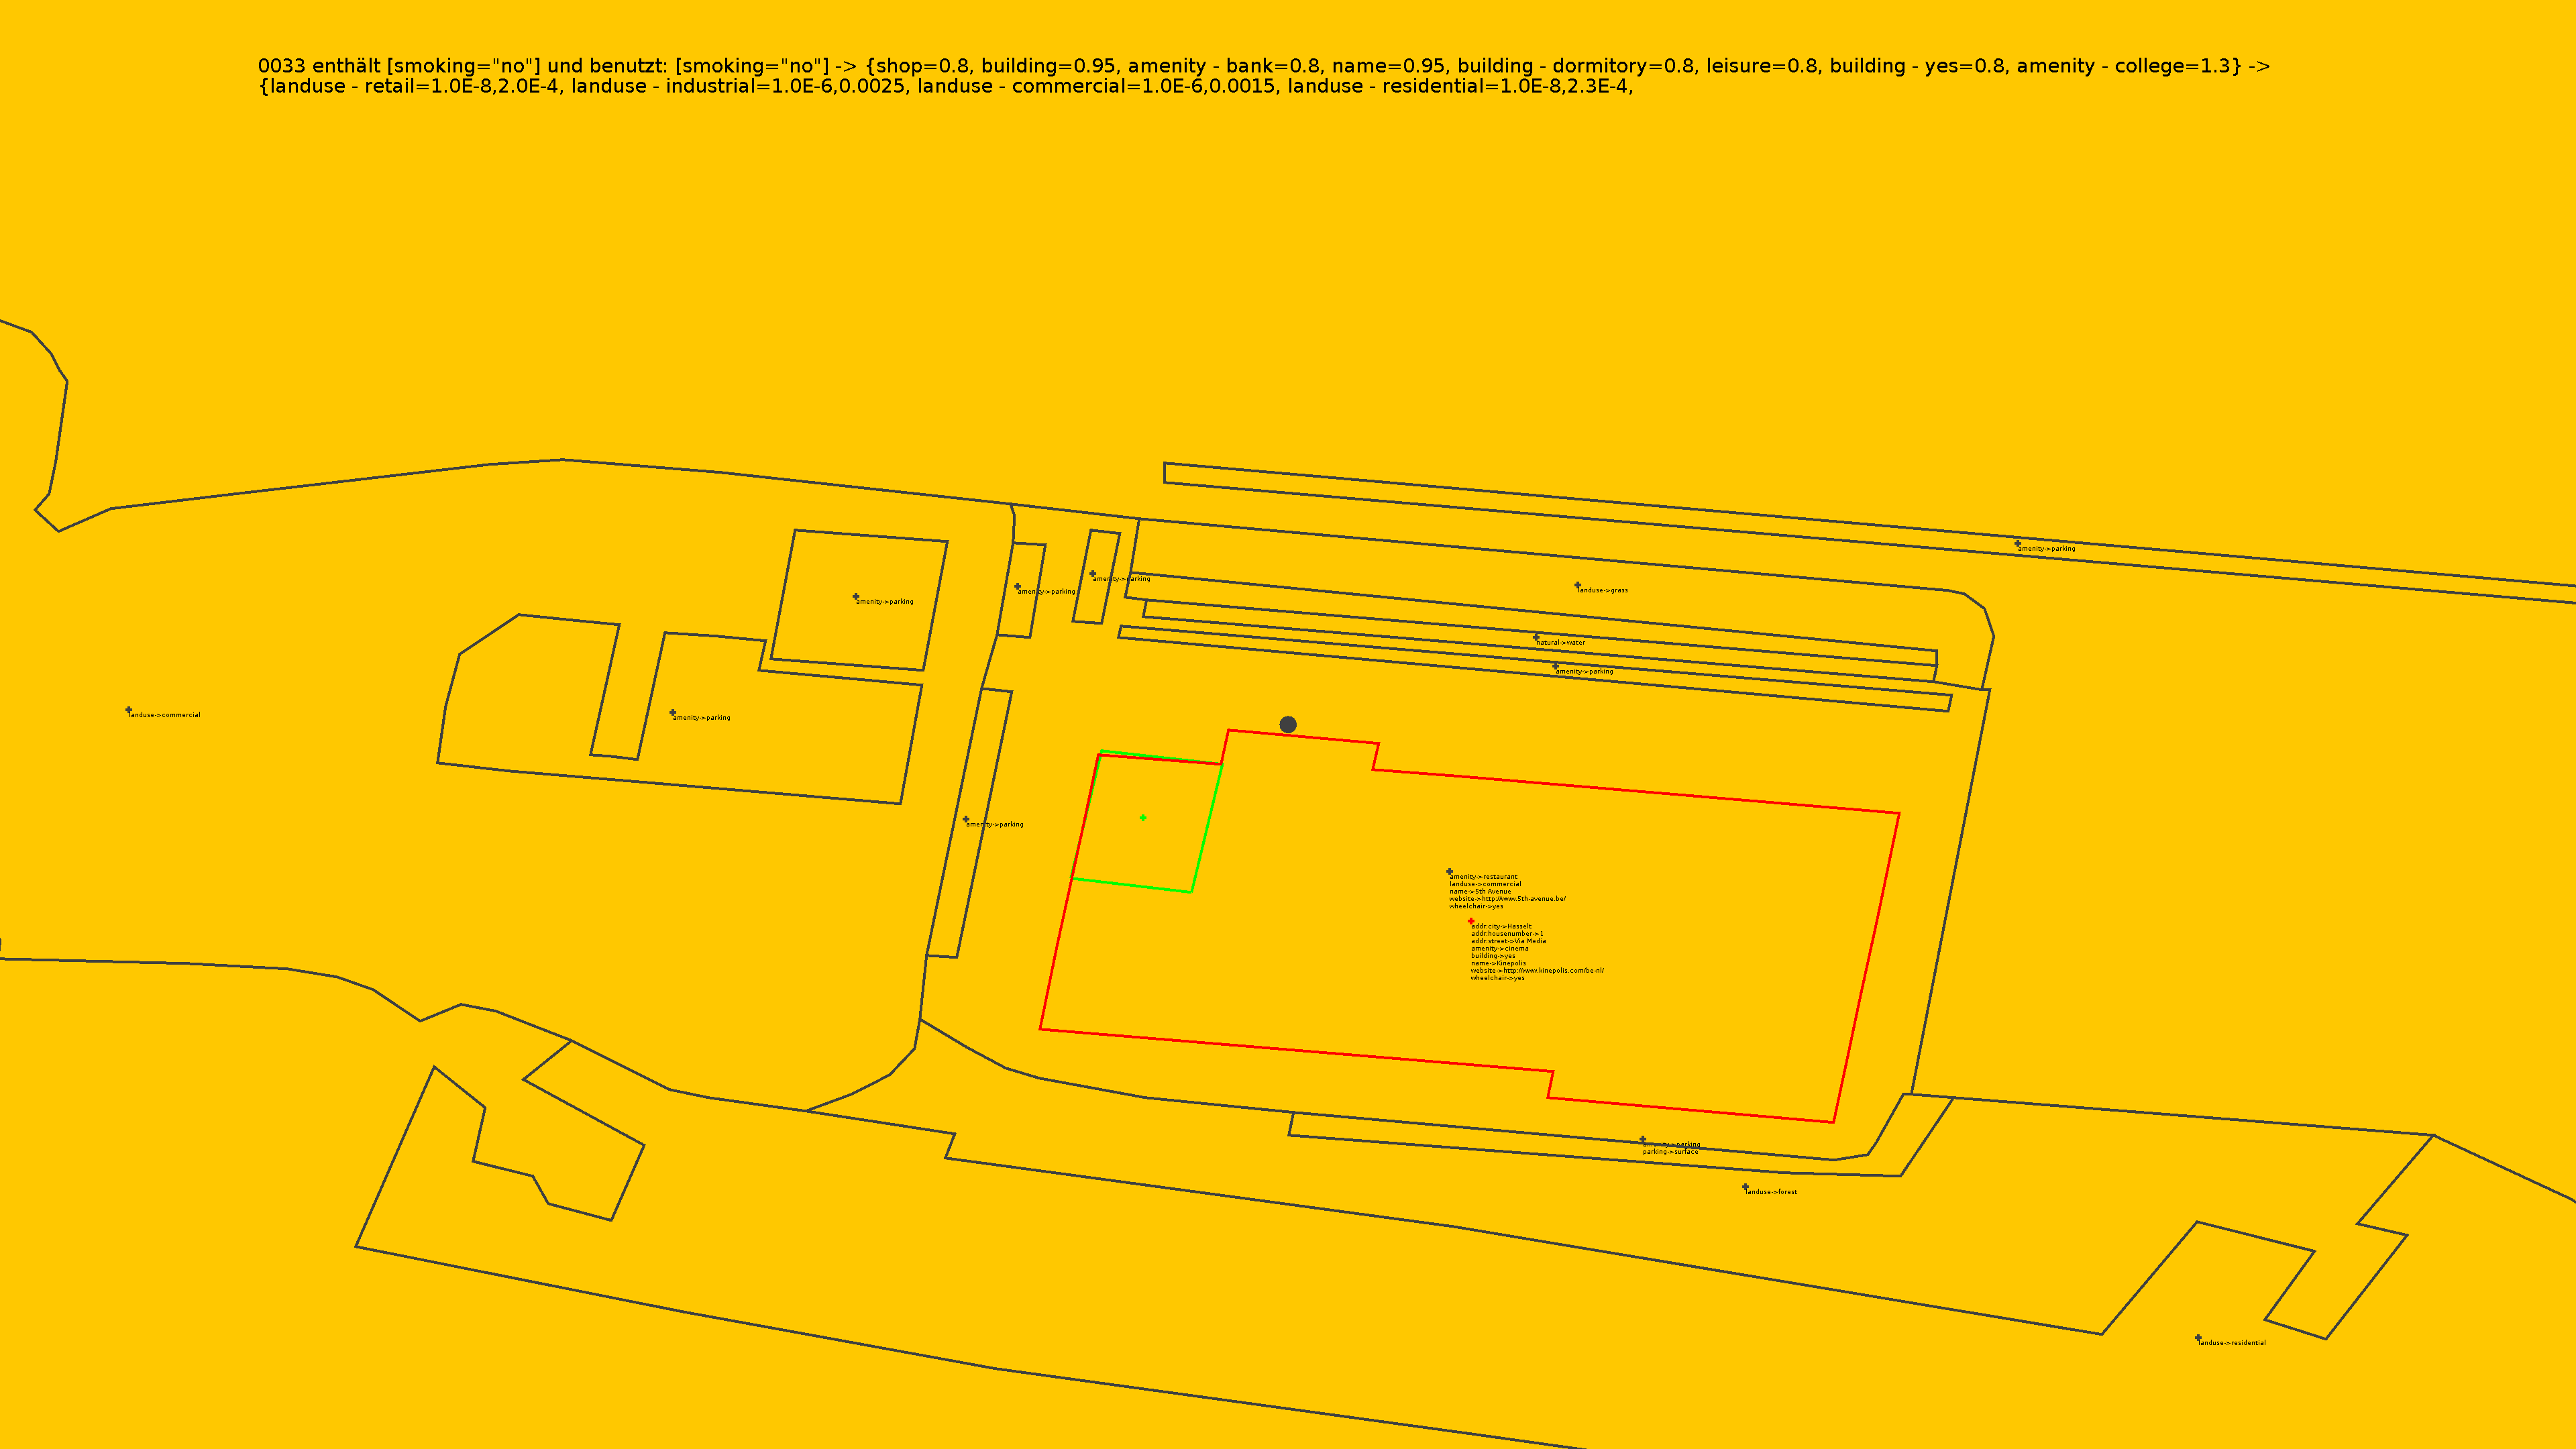
\includegraphics[width=\textwidth]{0033_big.png}}
\end{frame}


\begin{frame}
 \frametitle{Nicht geschafft}
  \Wider{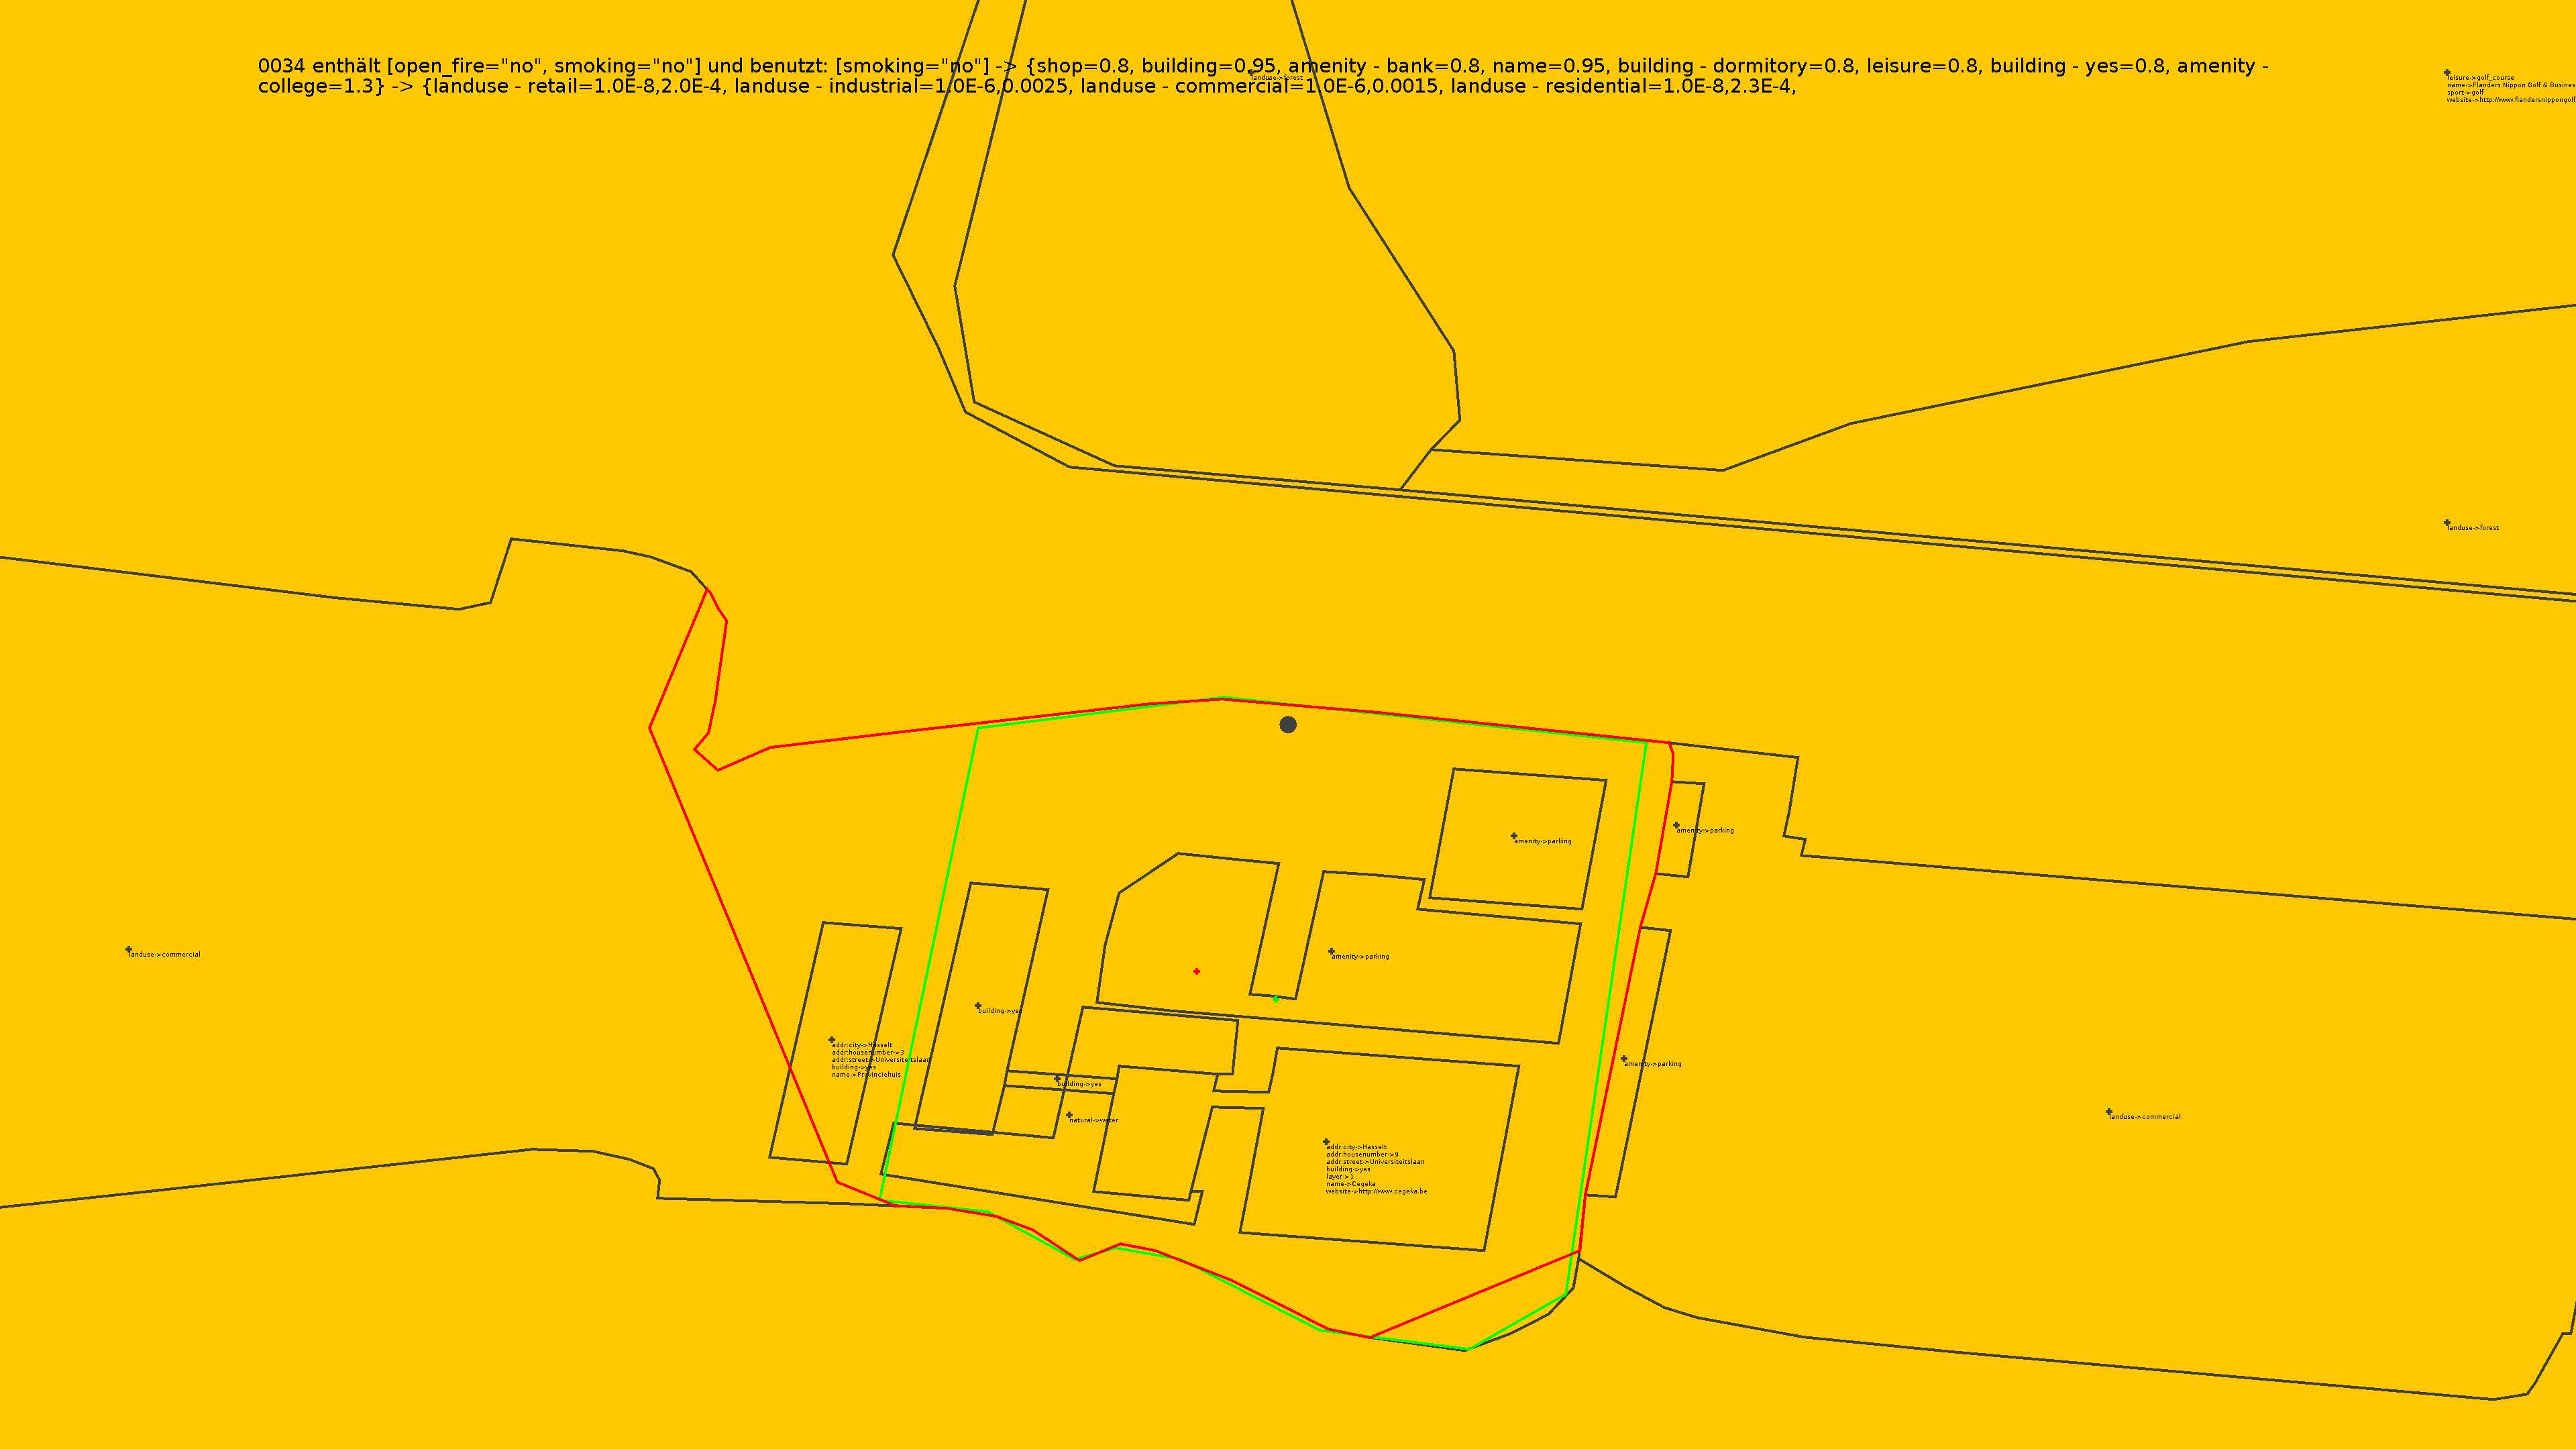
\includegraphics[width=\textwidth]{0034_big.png}}
\end{frame}


\begin{frame}
 \frametitle{Nicht geschafft}
  \Wider{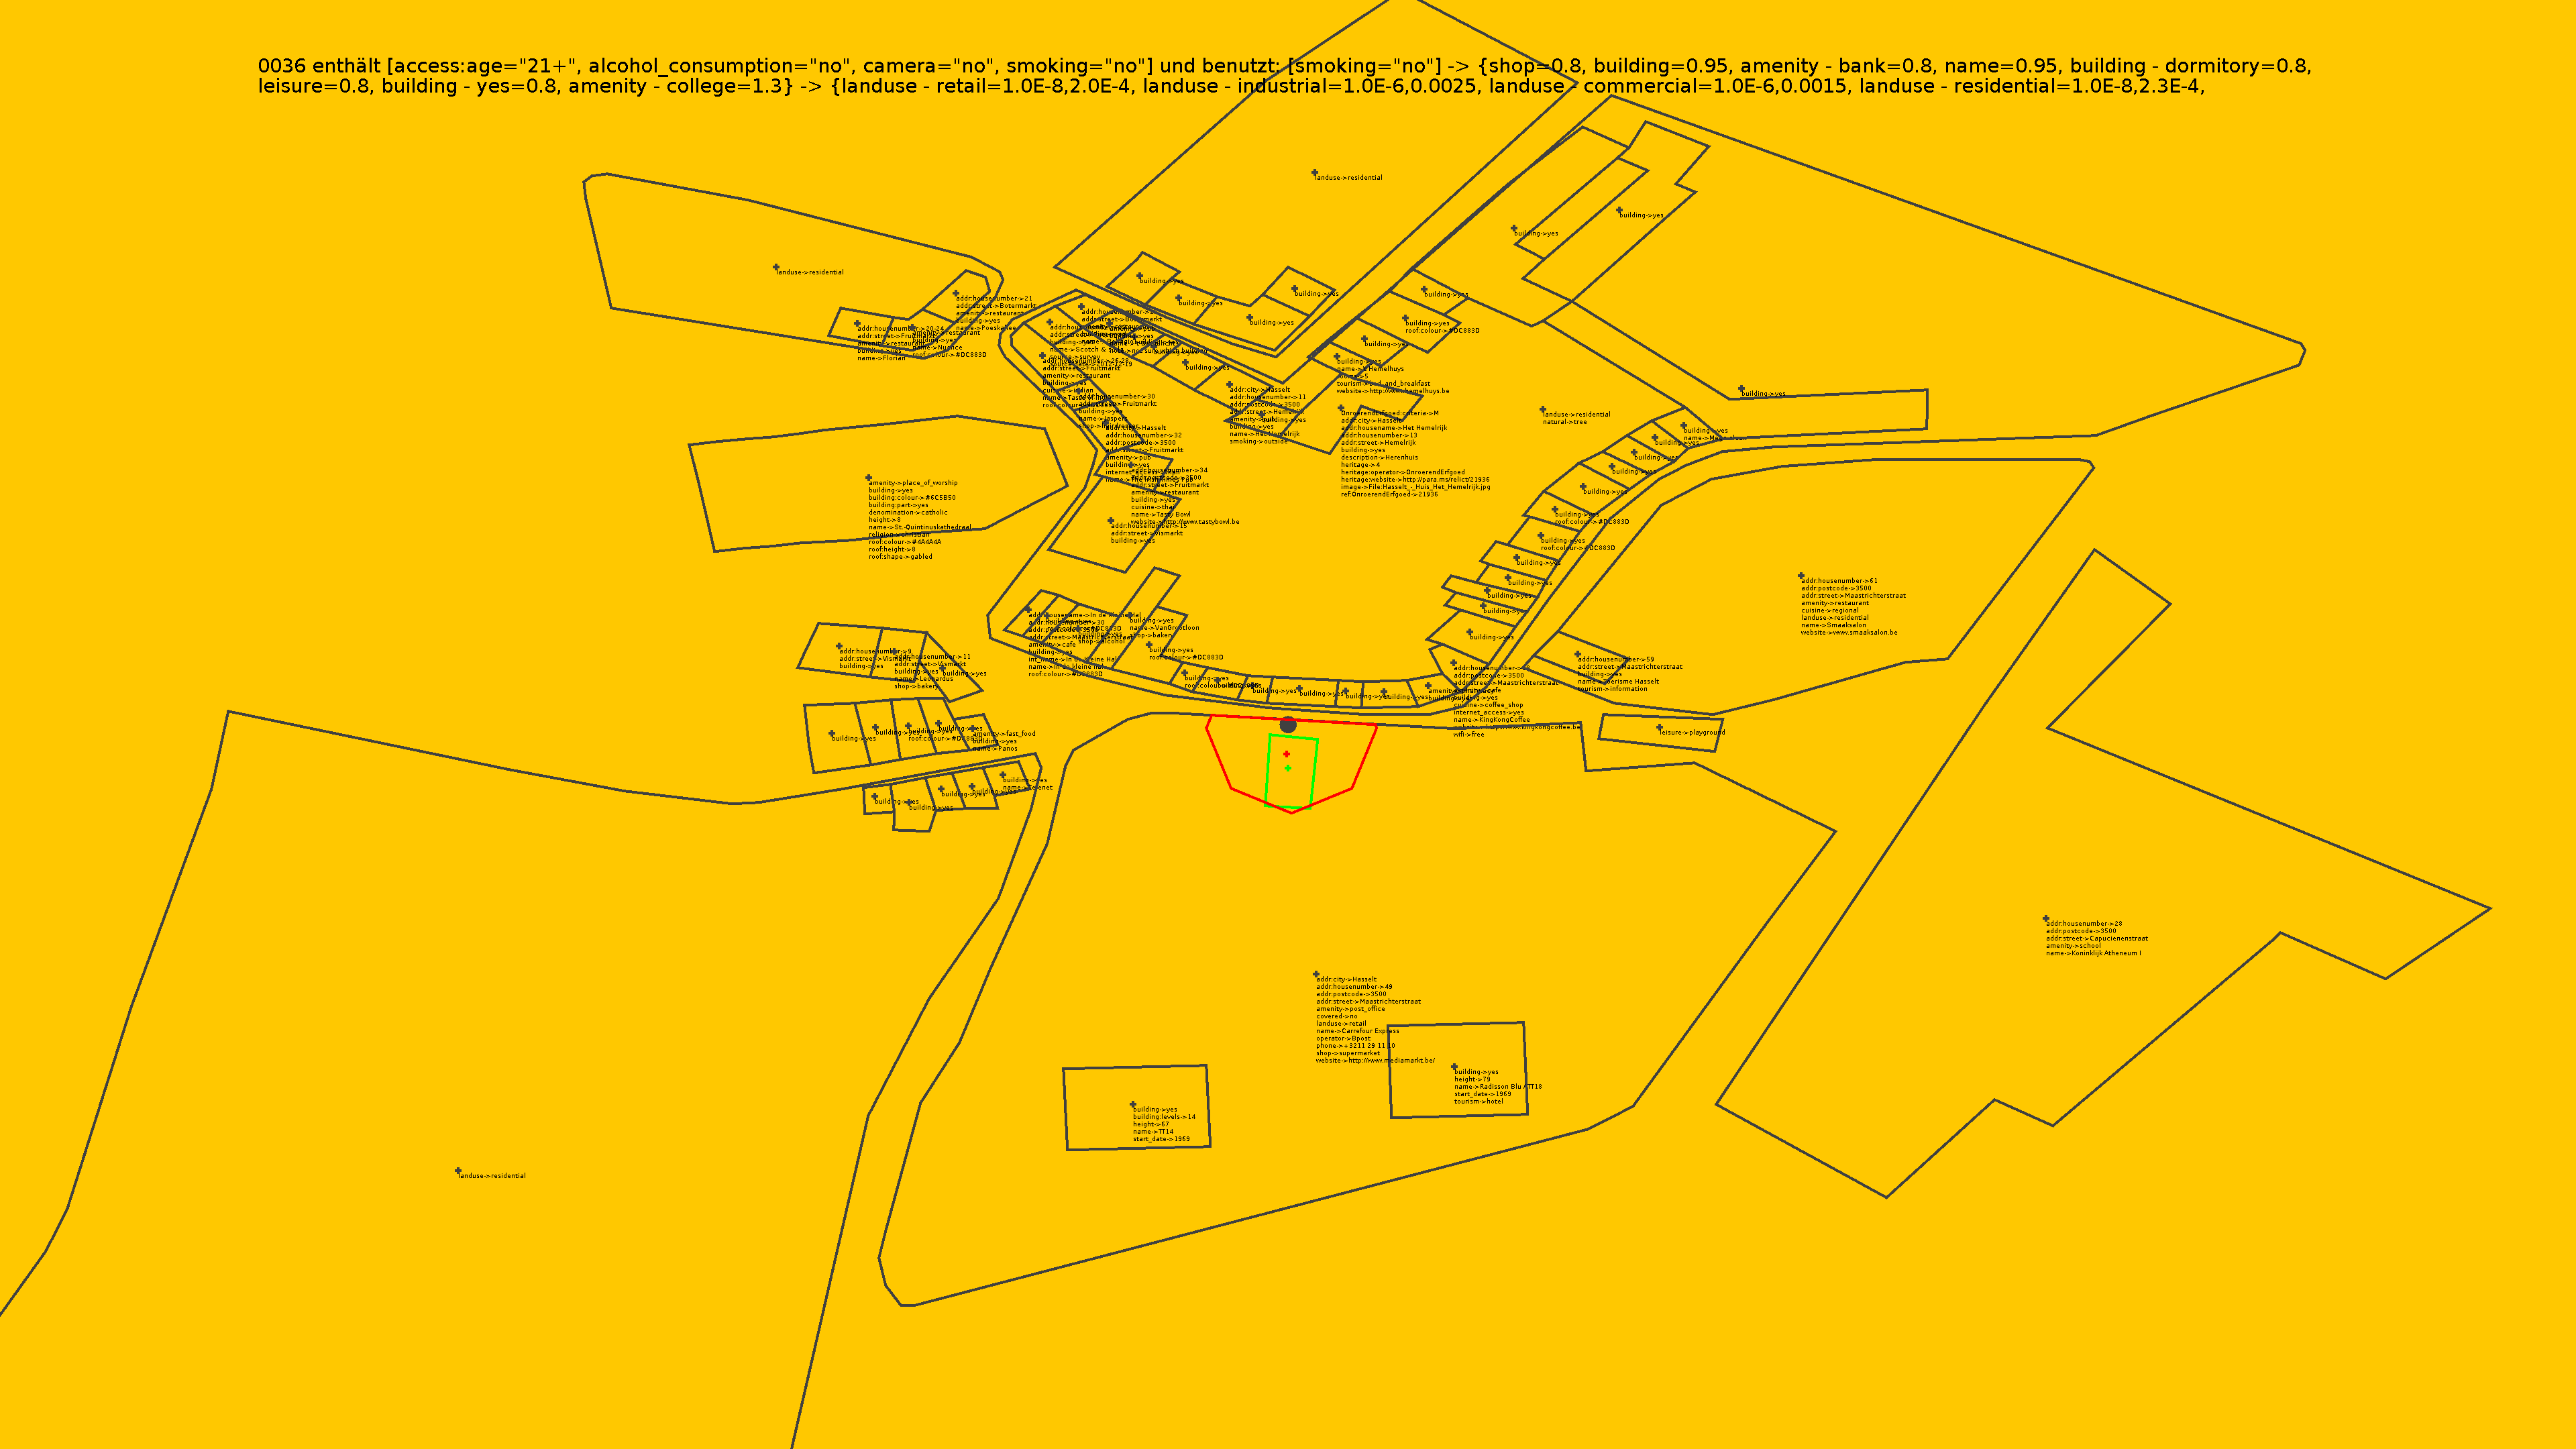
\includegraphics[width=\textwidth]{0036_big.png}}
\end{frame}


\begin{frame}
 \frametitle{Nicht geschafft}
  \Wider{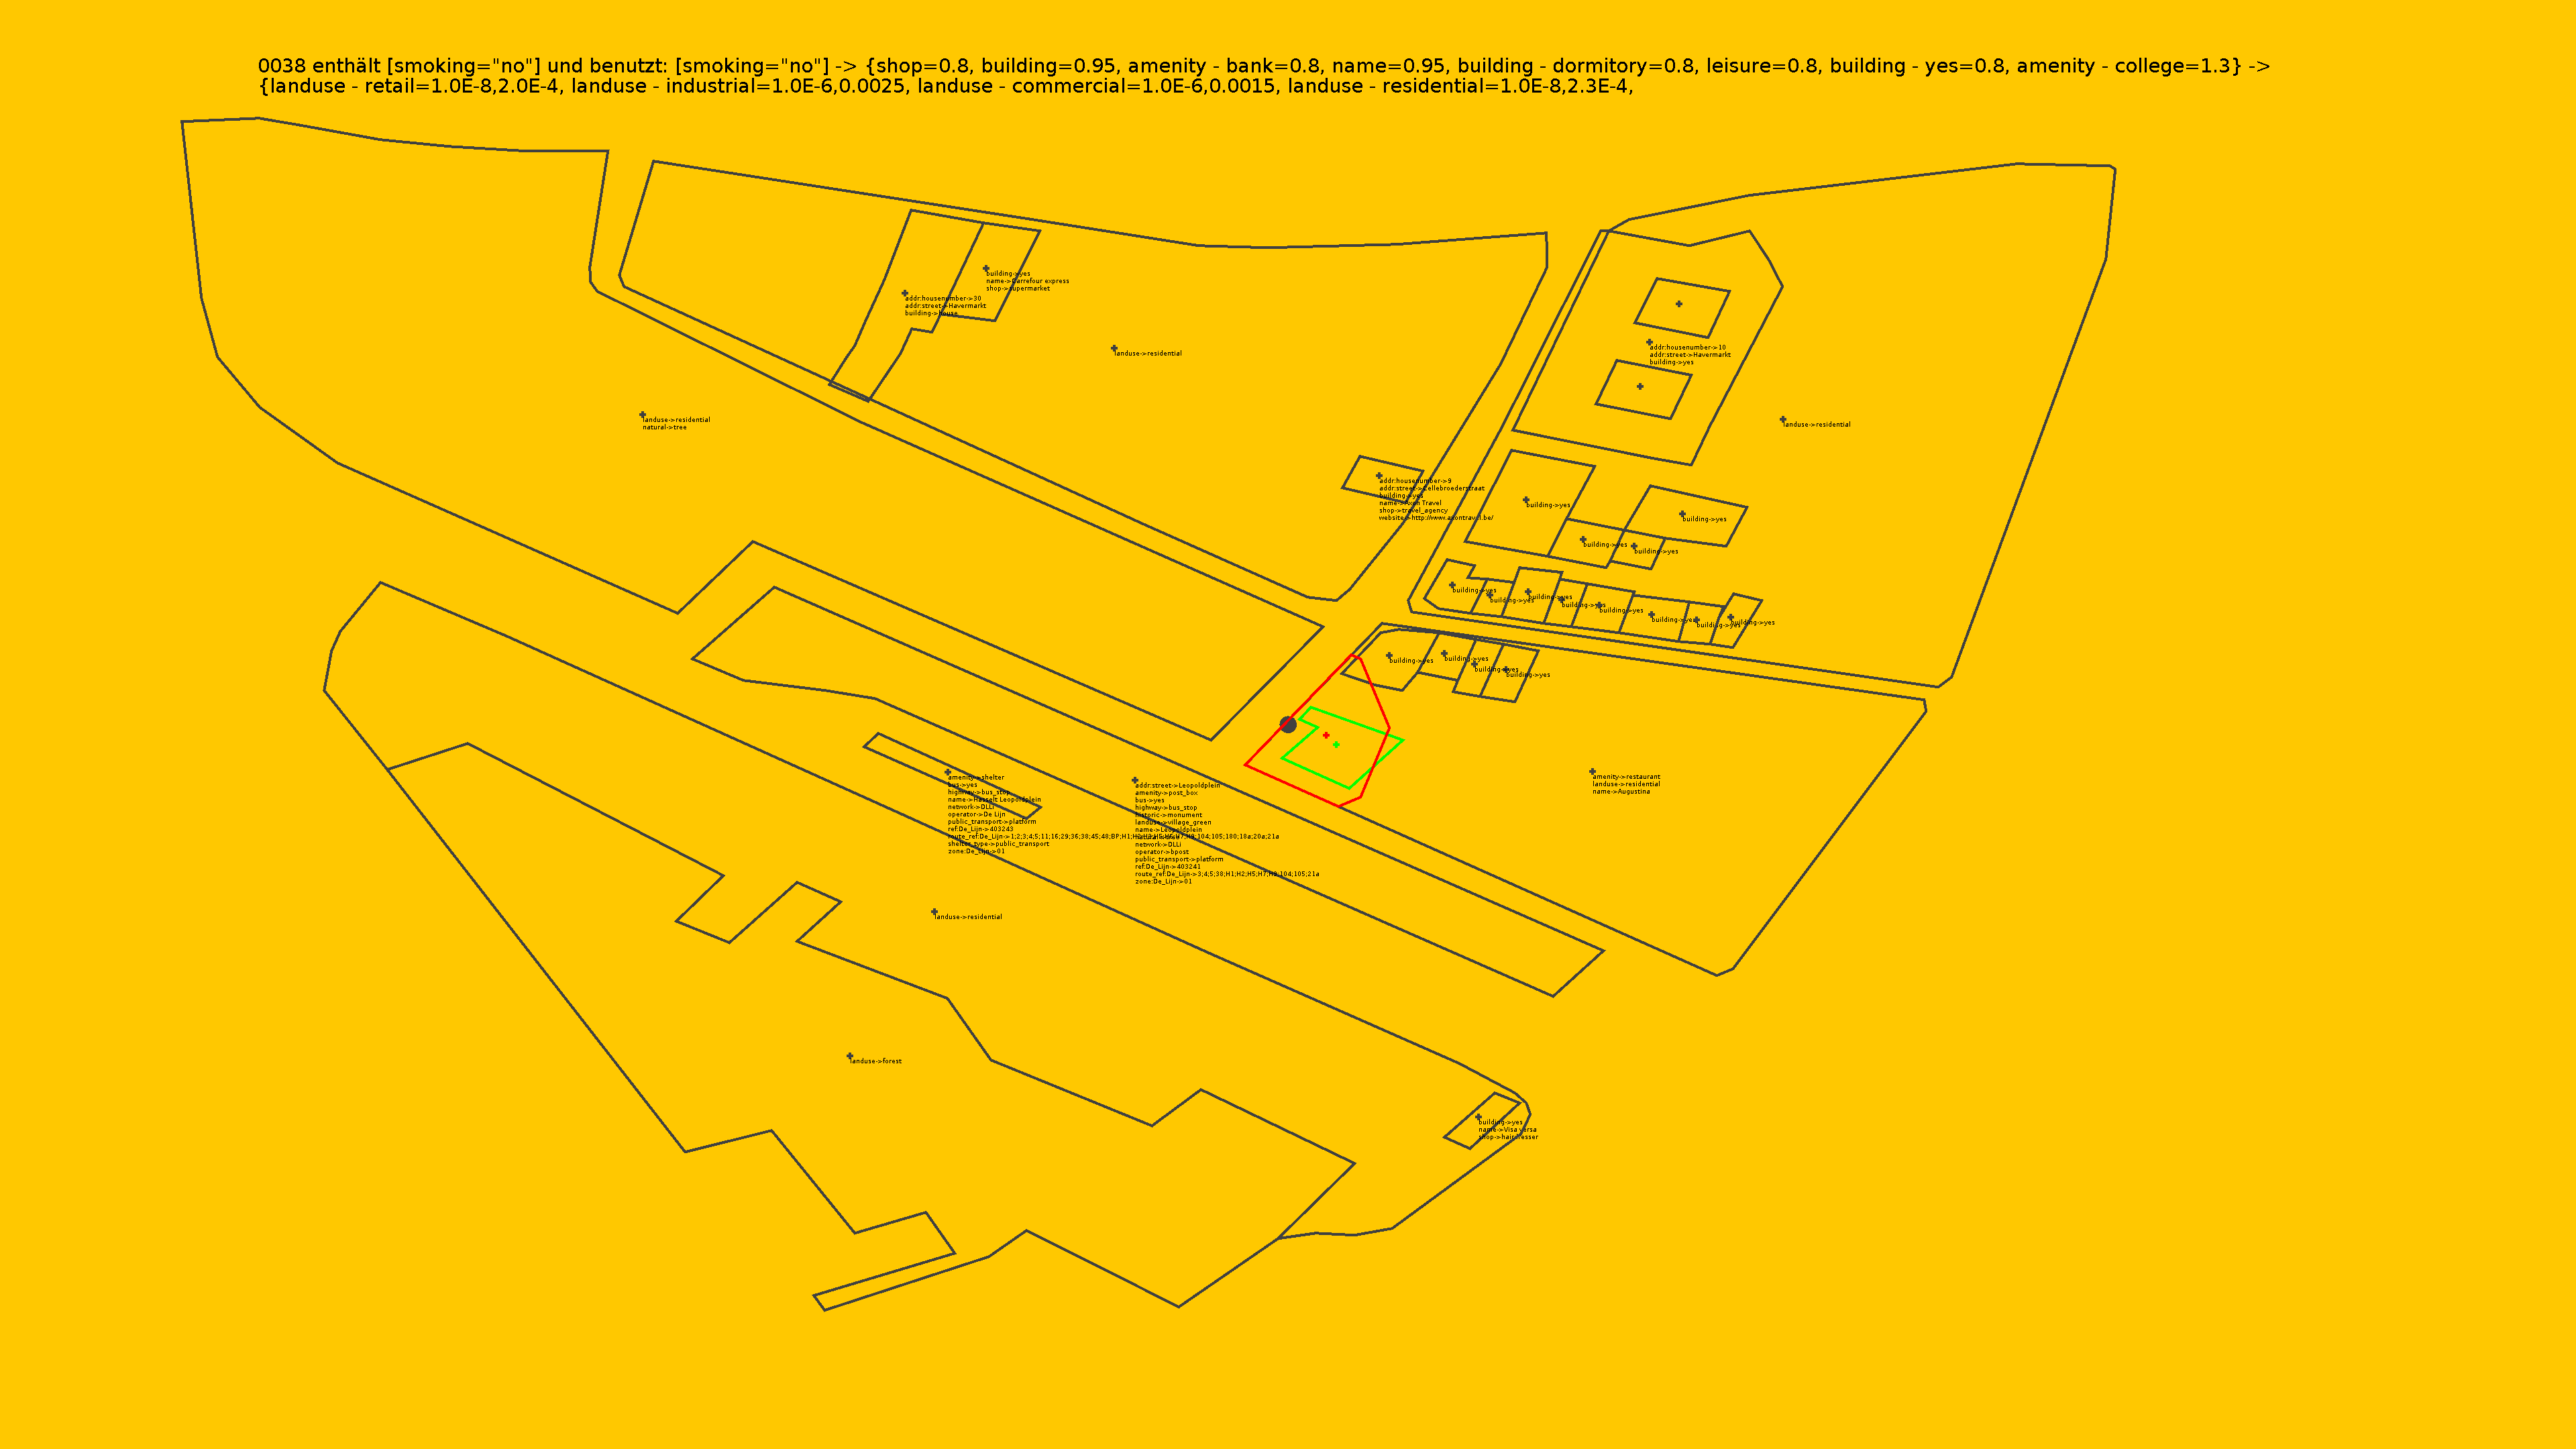
\includegraphics[width=\textwidth]{0038_big.png}}
\end{frame}


\begin{frame}
 \frametitle{Nicht geschafft}
  \Wider{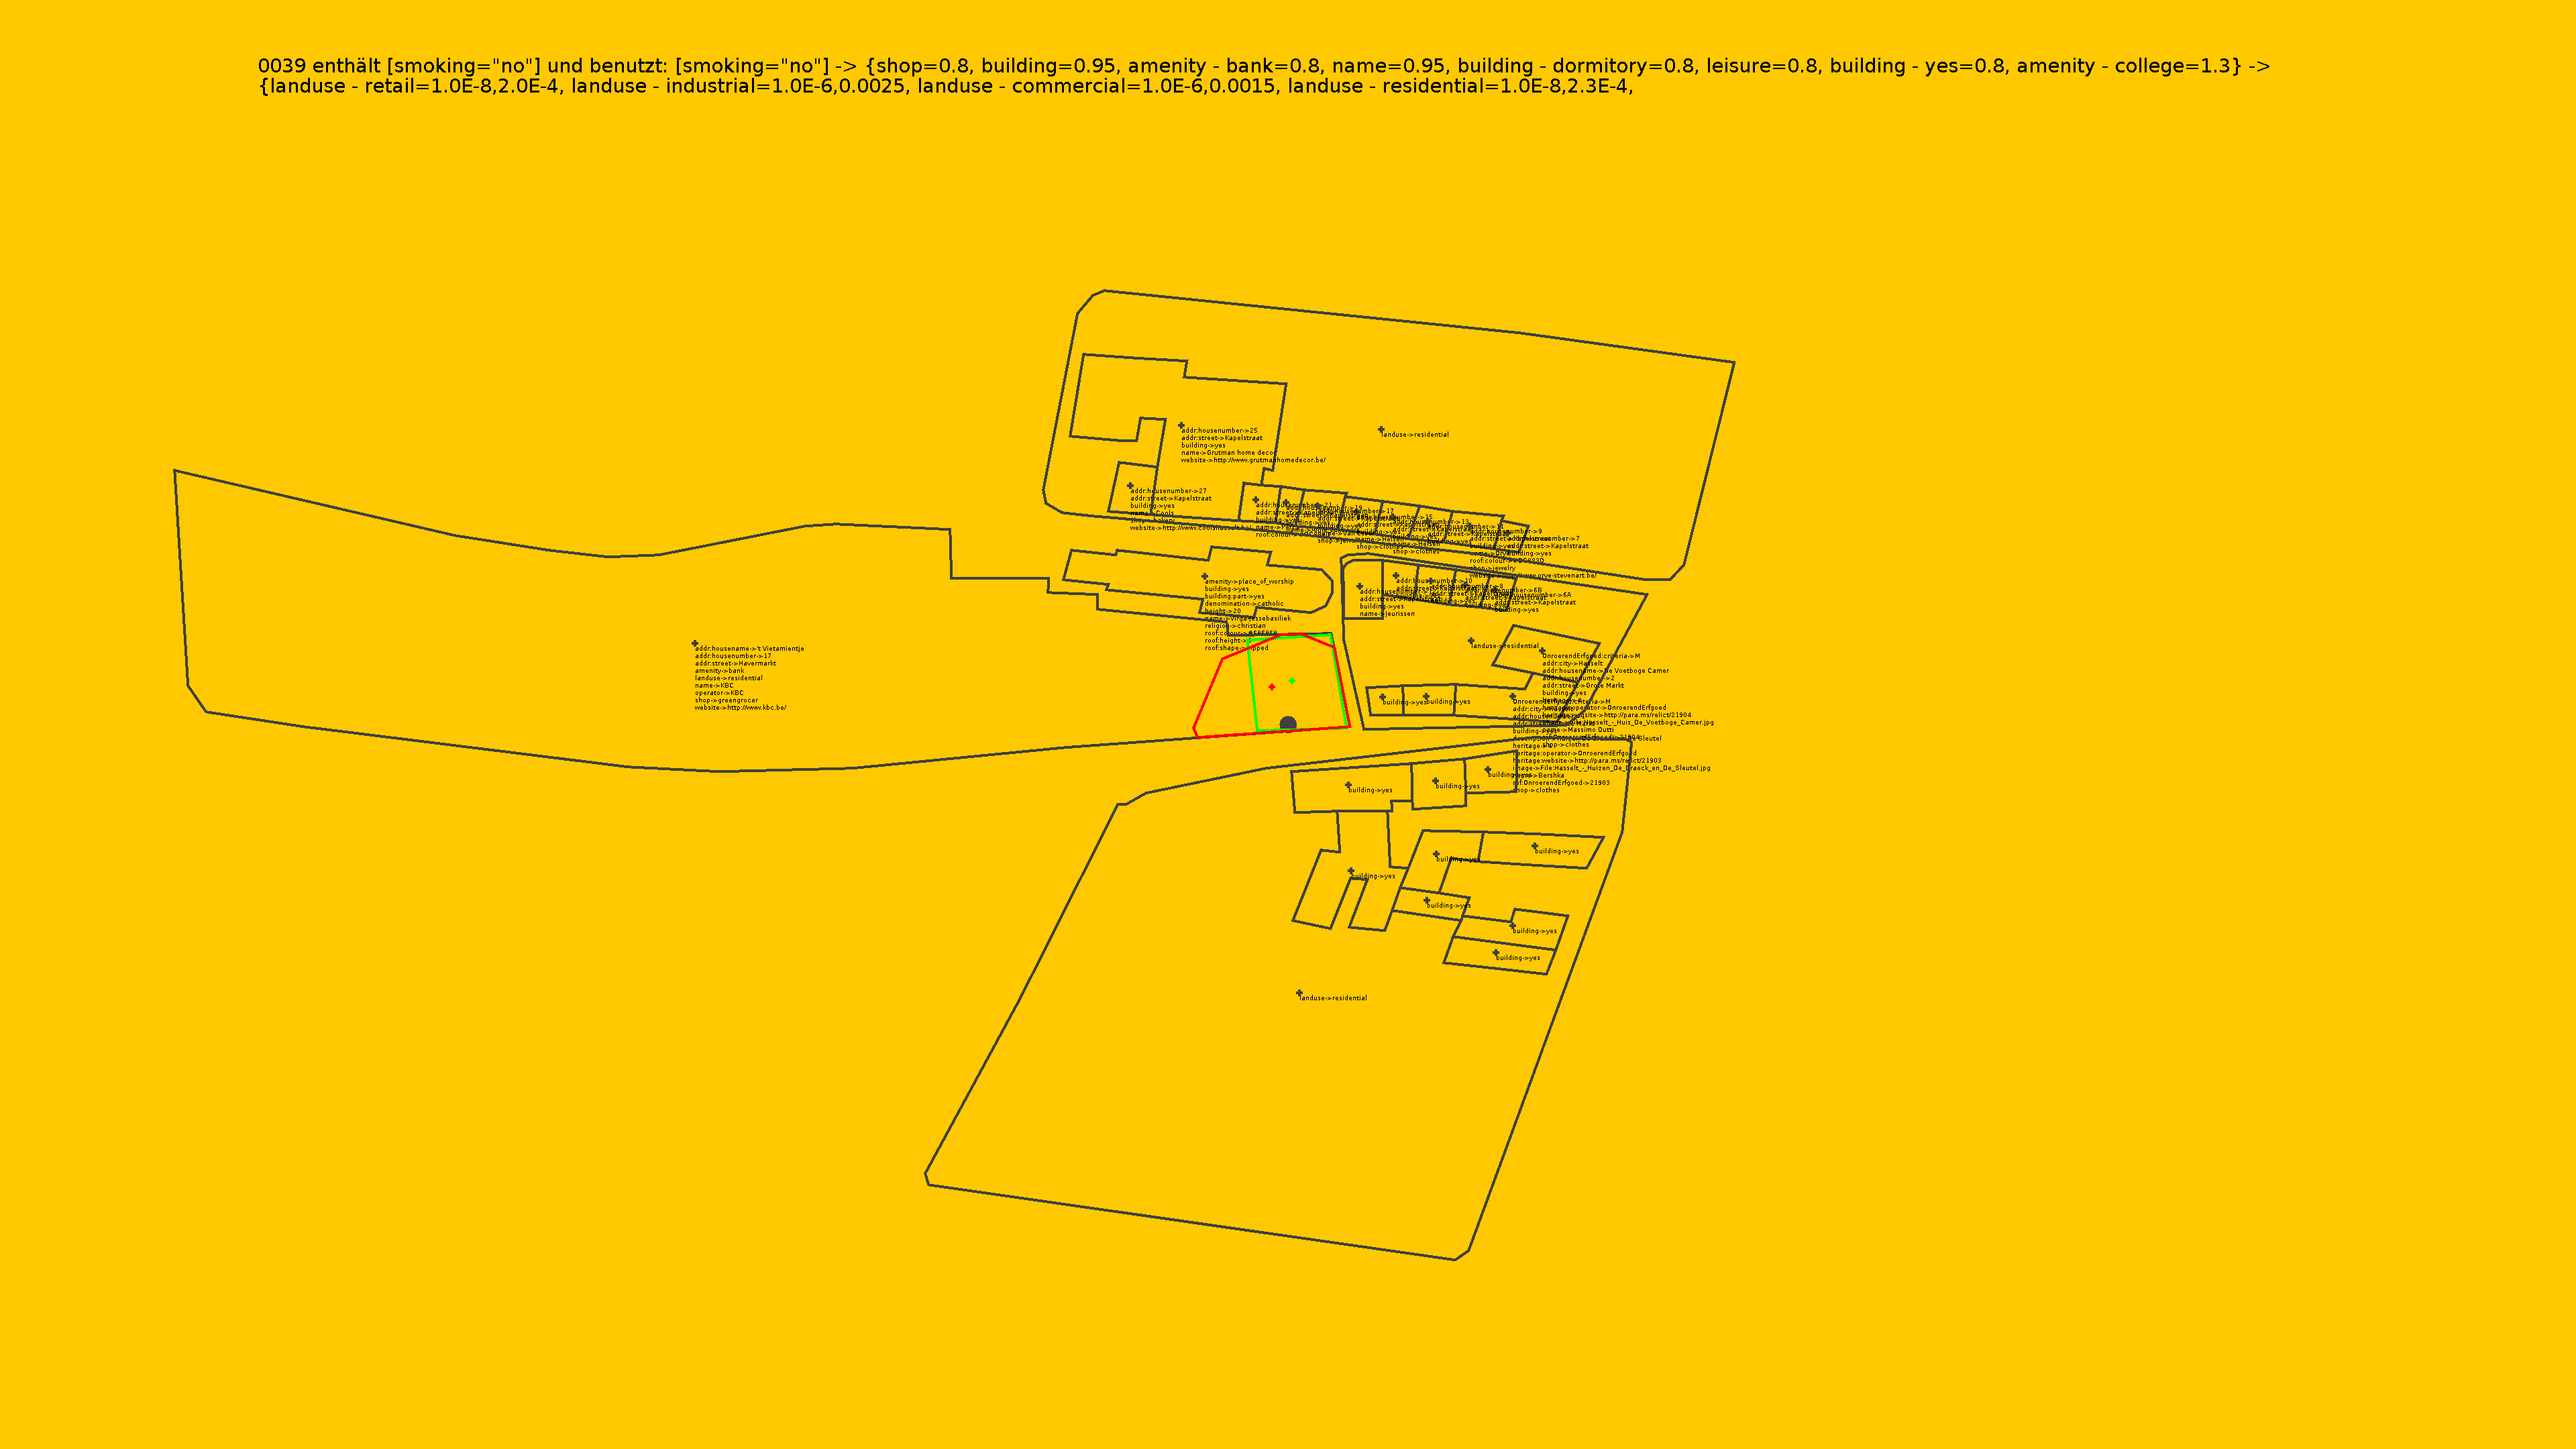
\includegraphics[width=\textwidth]{0039_big.png}}
\end{frame}


\begin{frame}
 \frametitle{Nicht geschafft}
  \Wider{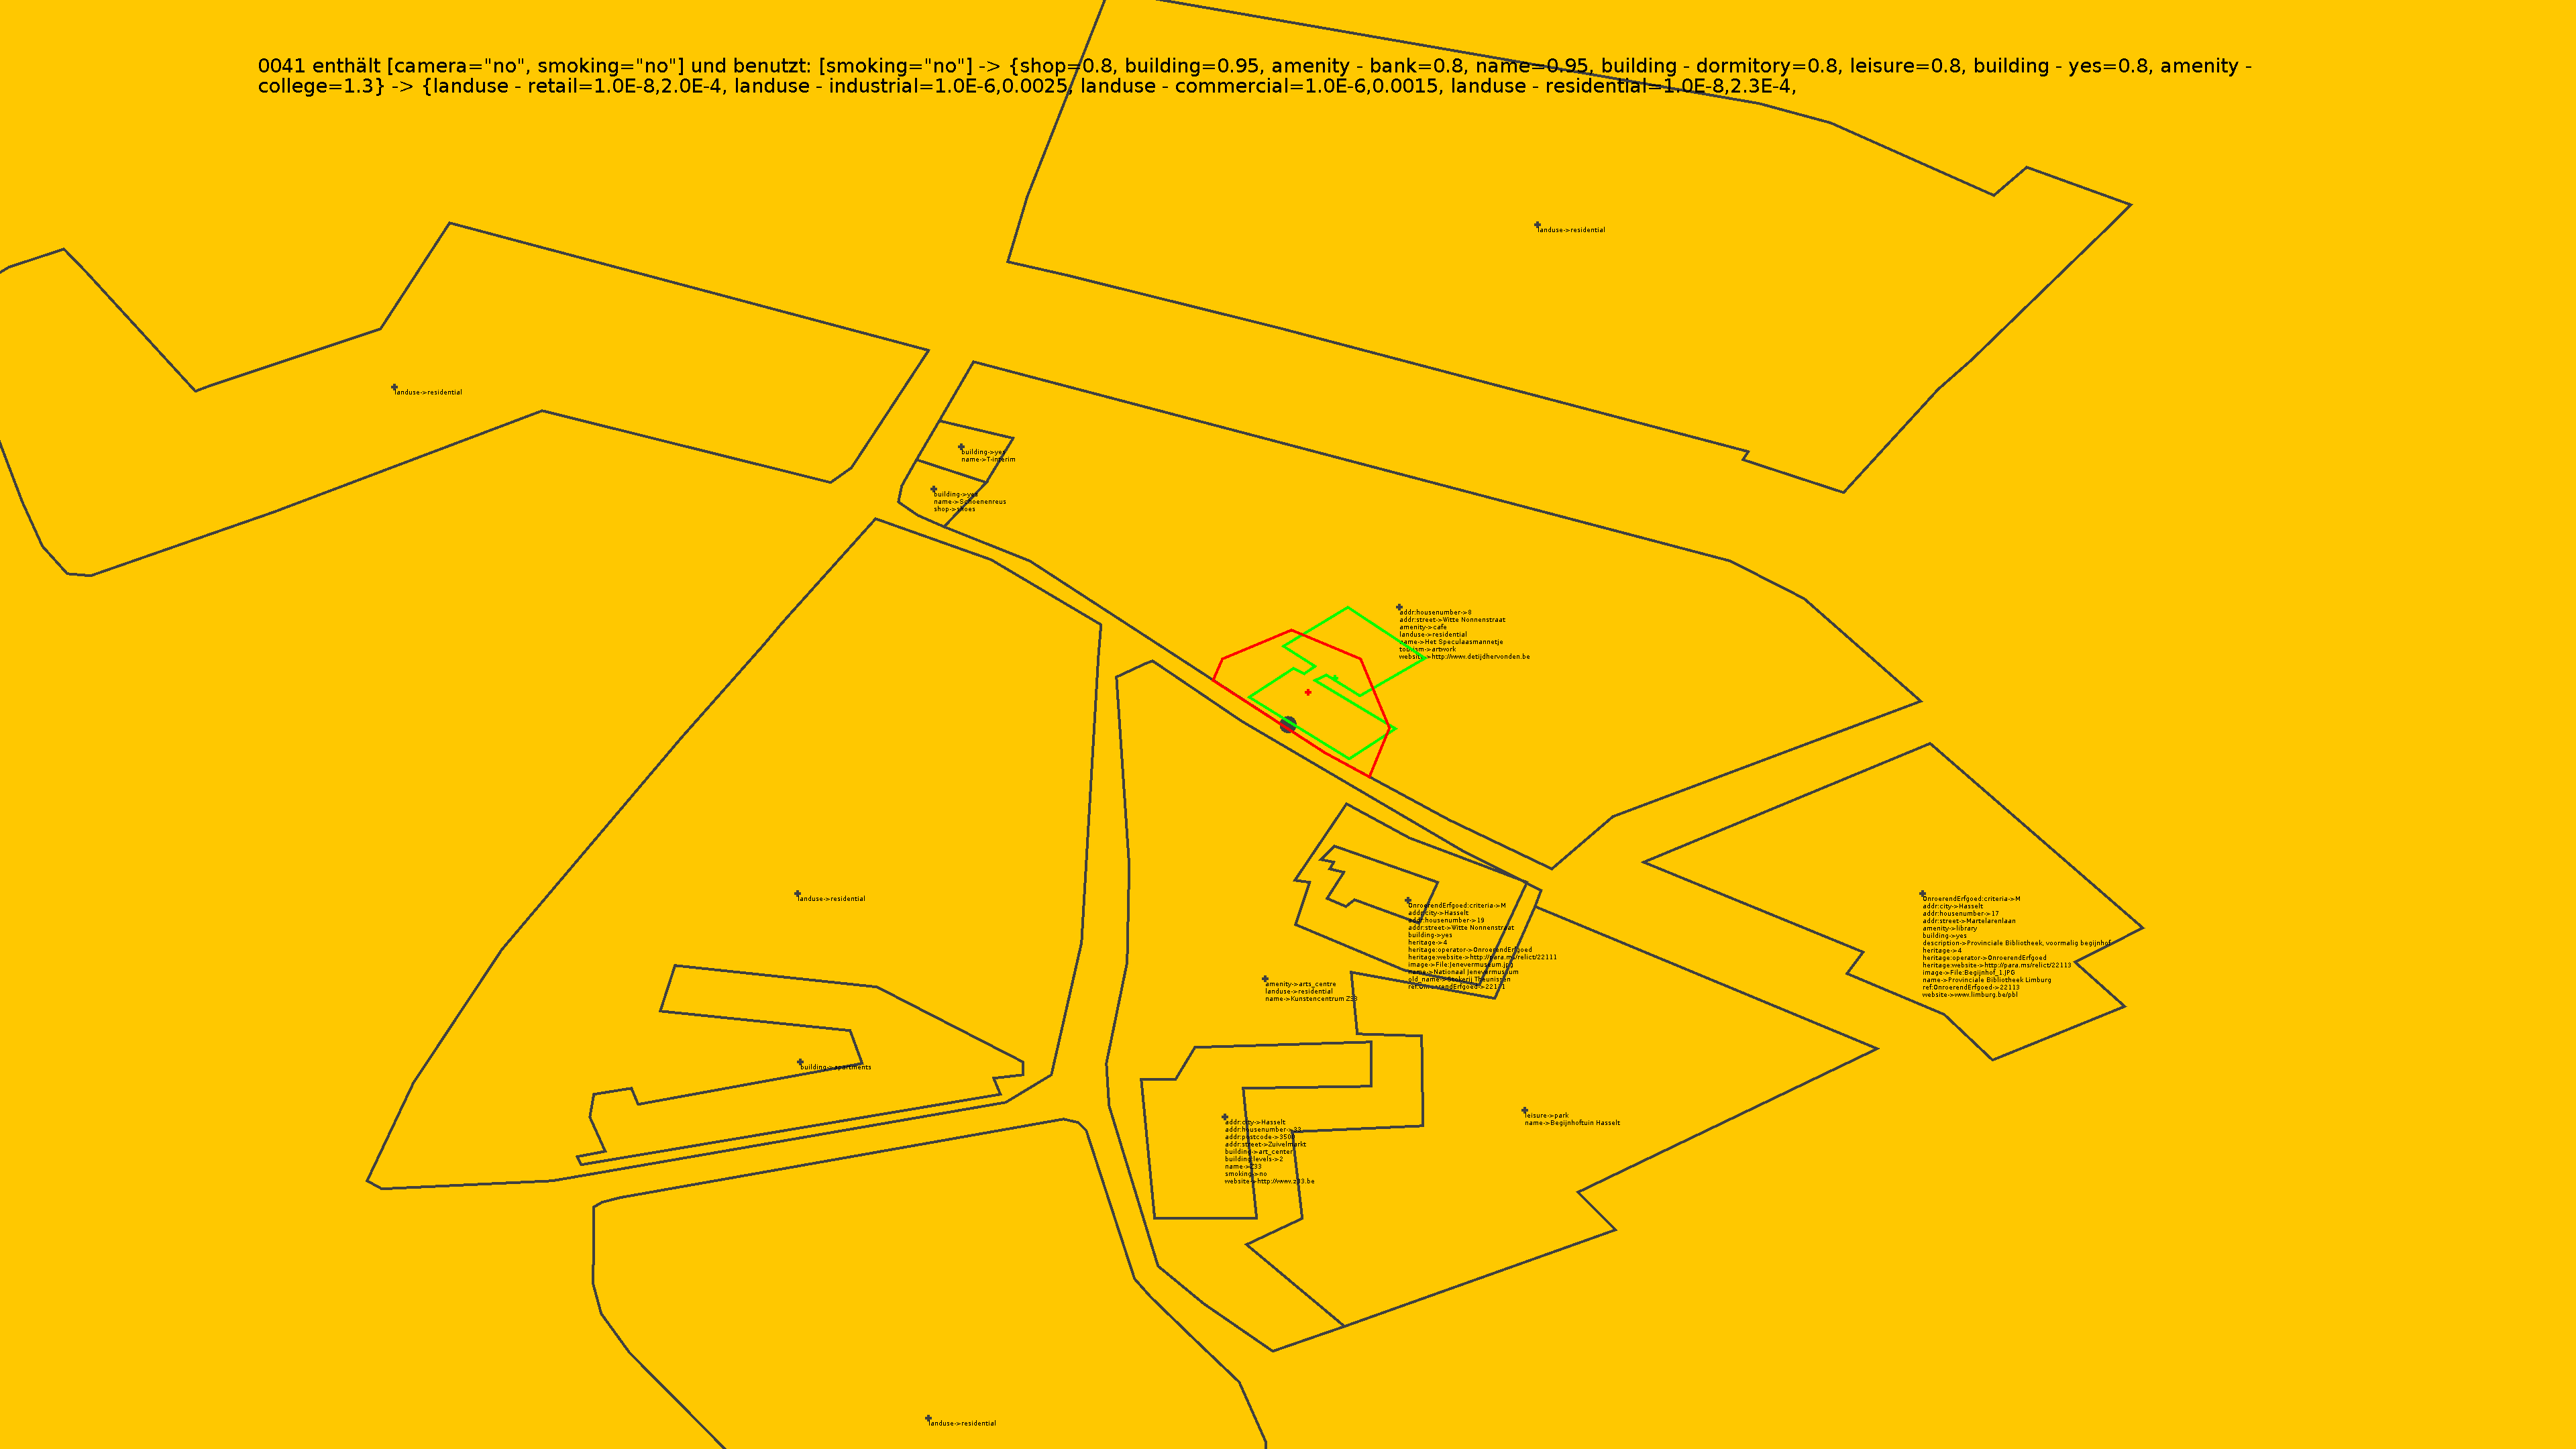
\includegraphics[width=\textwidth]{0041_big.png}}
\end{frame}


\begin{frame}
 \frametitle{Nicht geschafft}
  \Wider{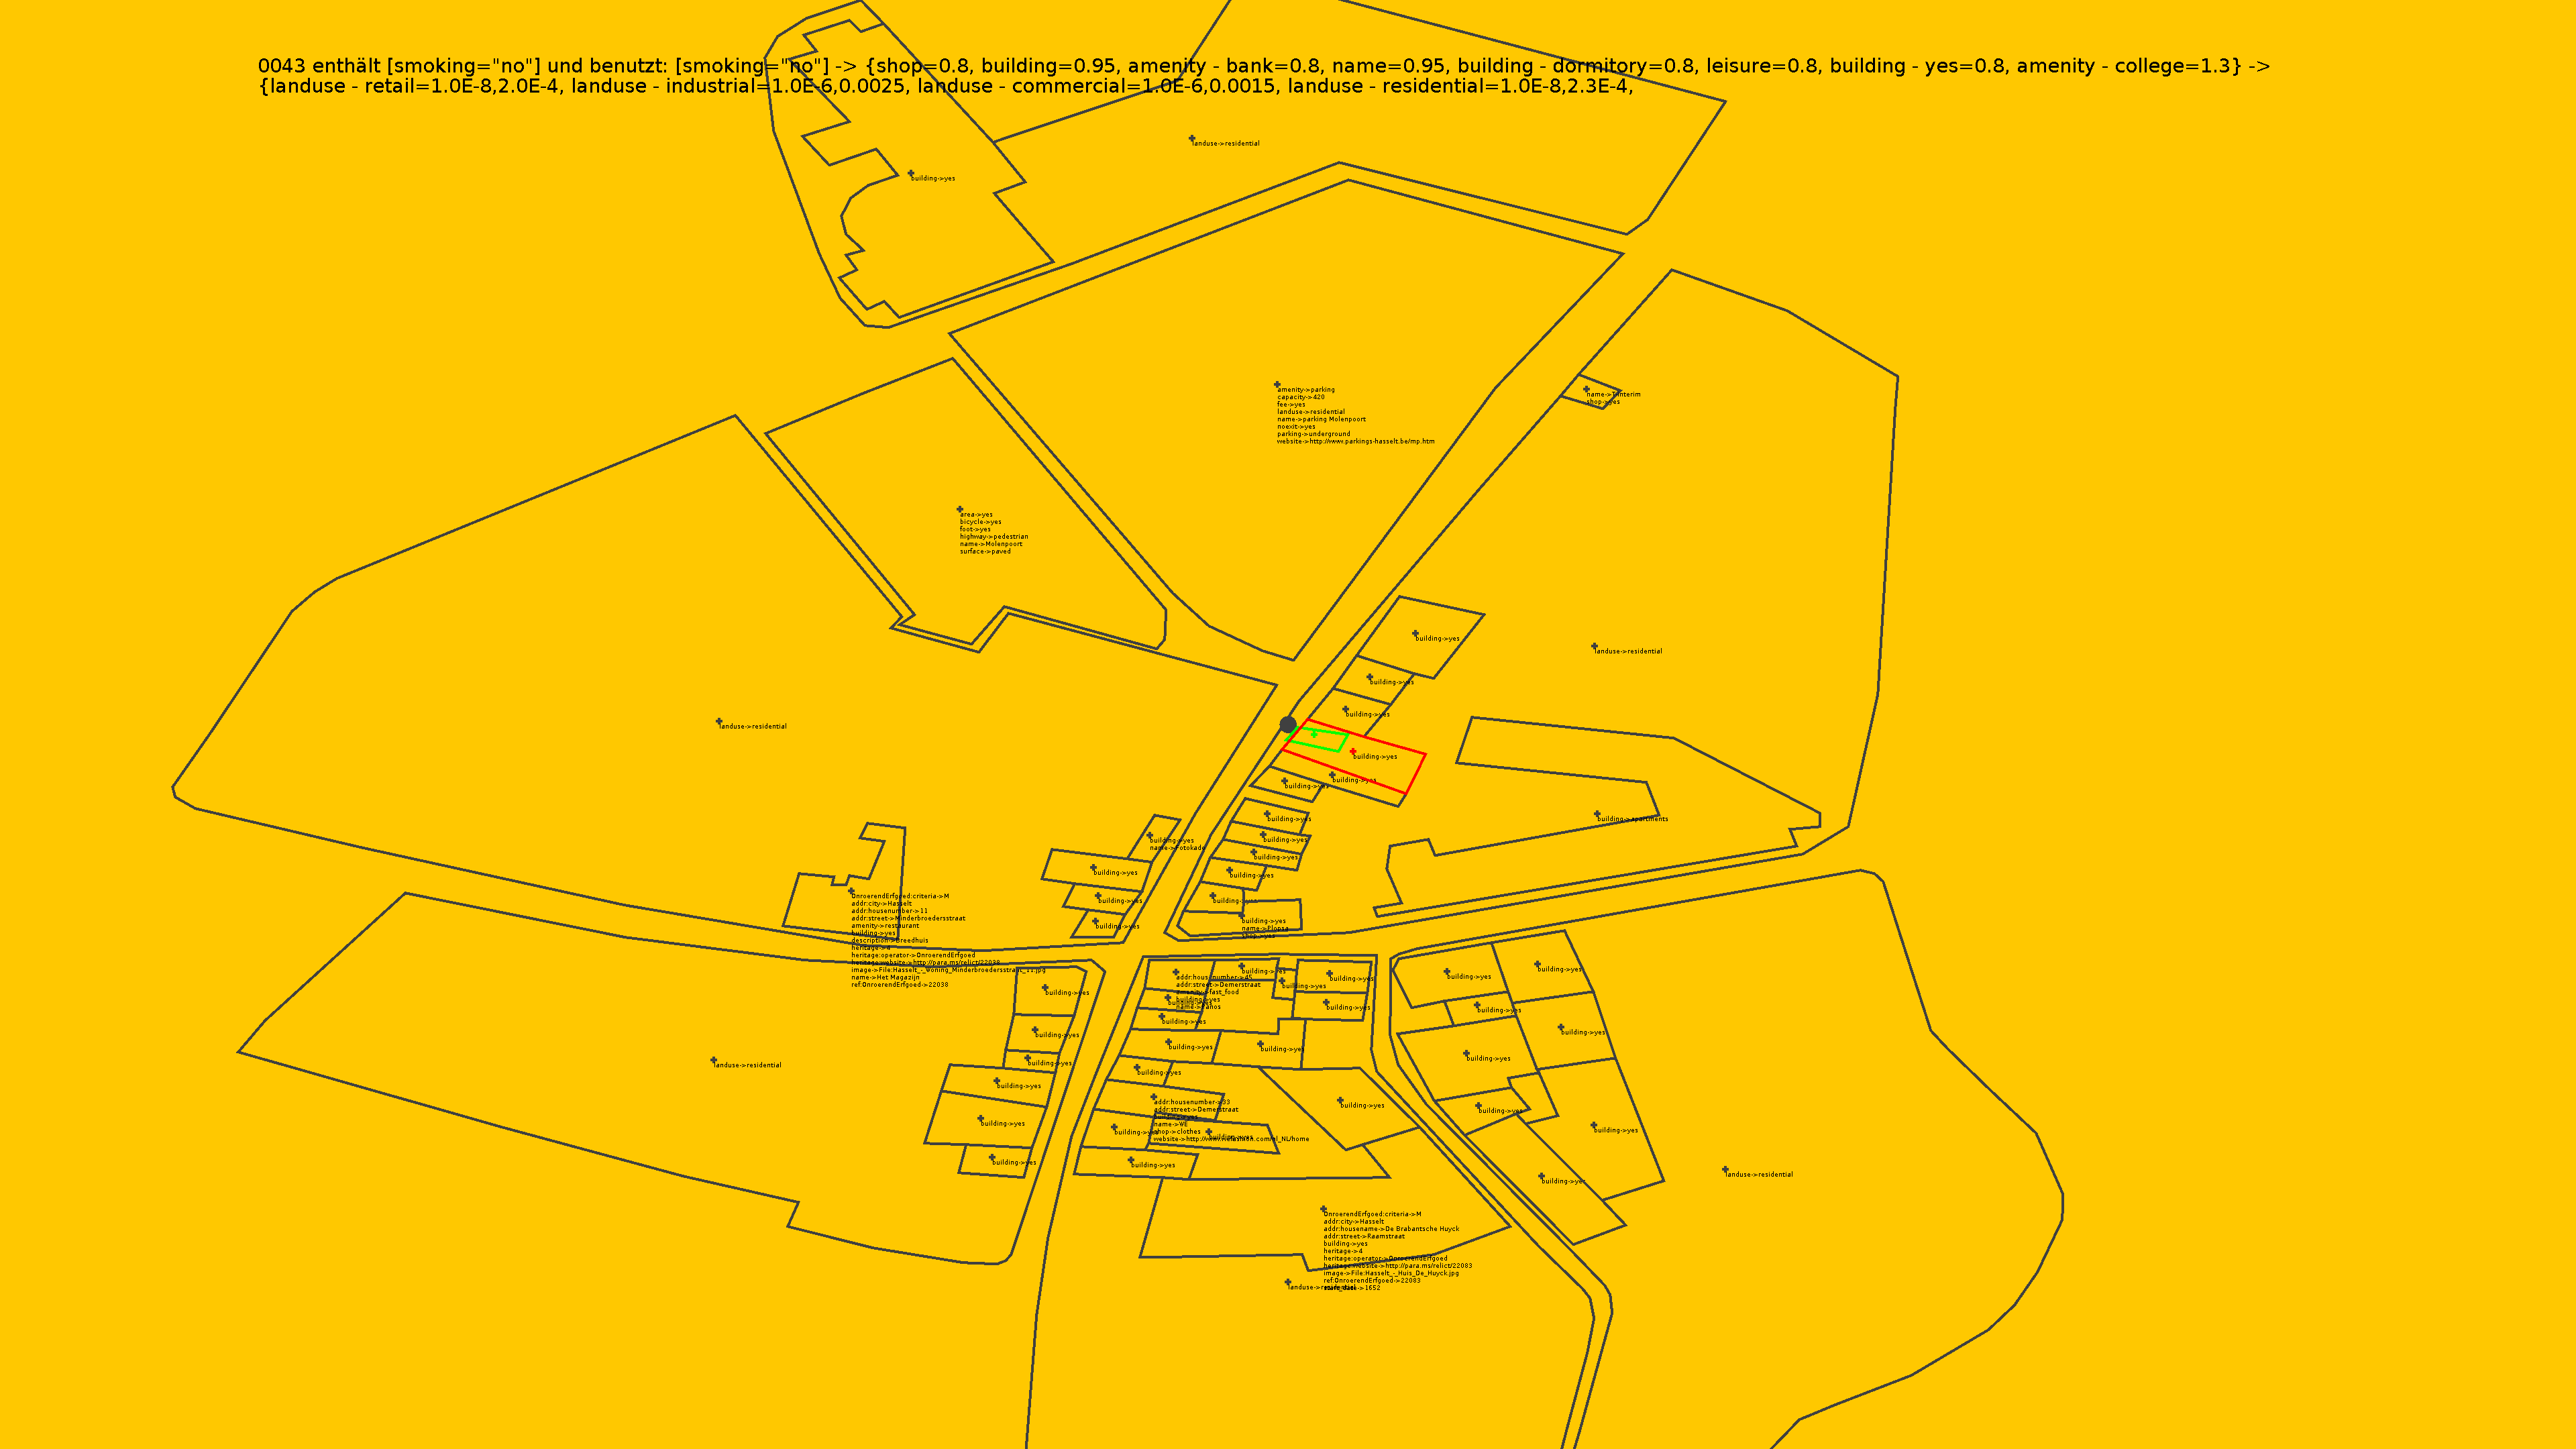
\includegraphics[width=\textwidth]{0043_big.png}}
\end{frame}


\begin{frame}
 \frametitle{Nicht geschafft}
  \Wider{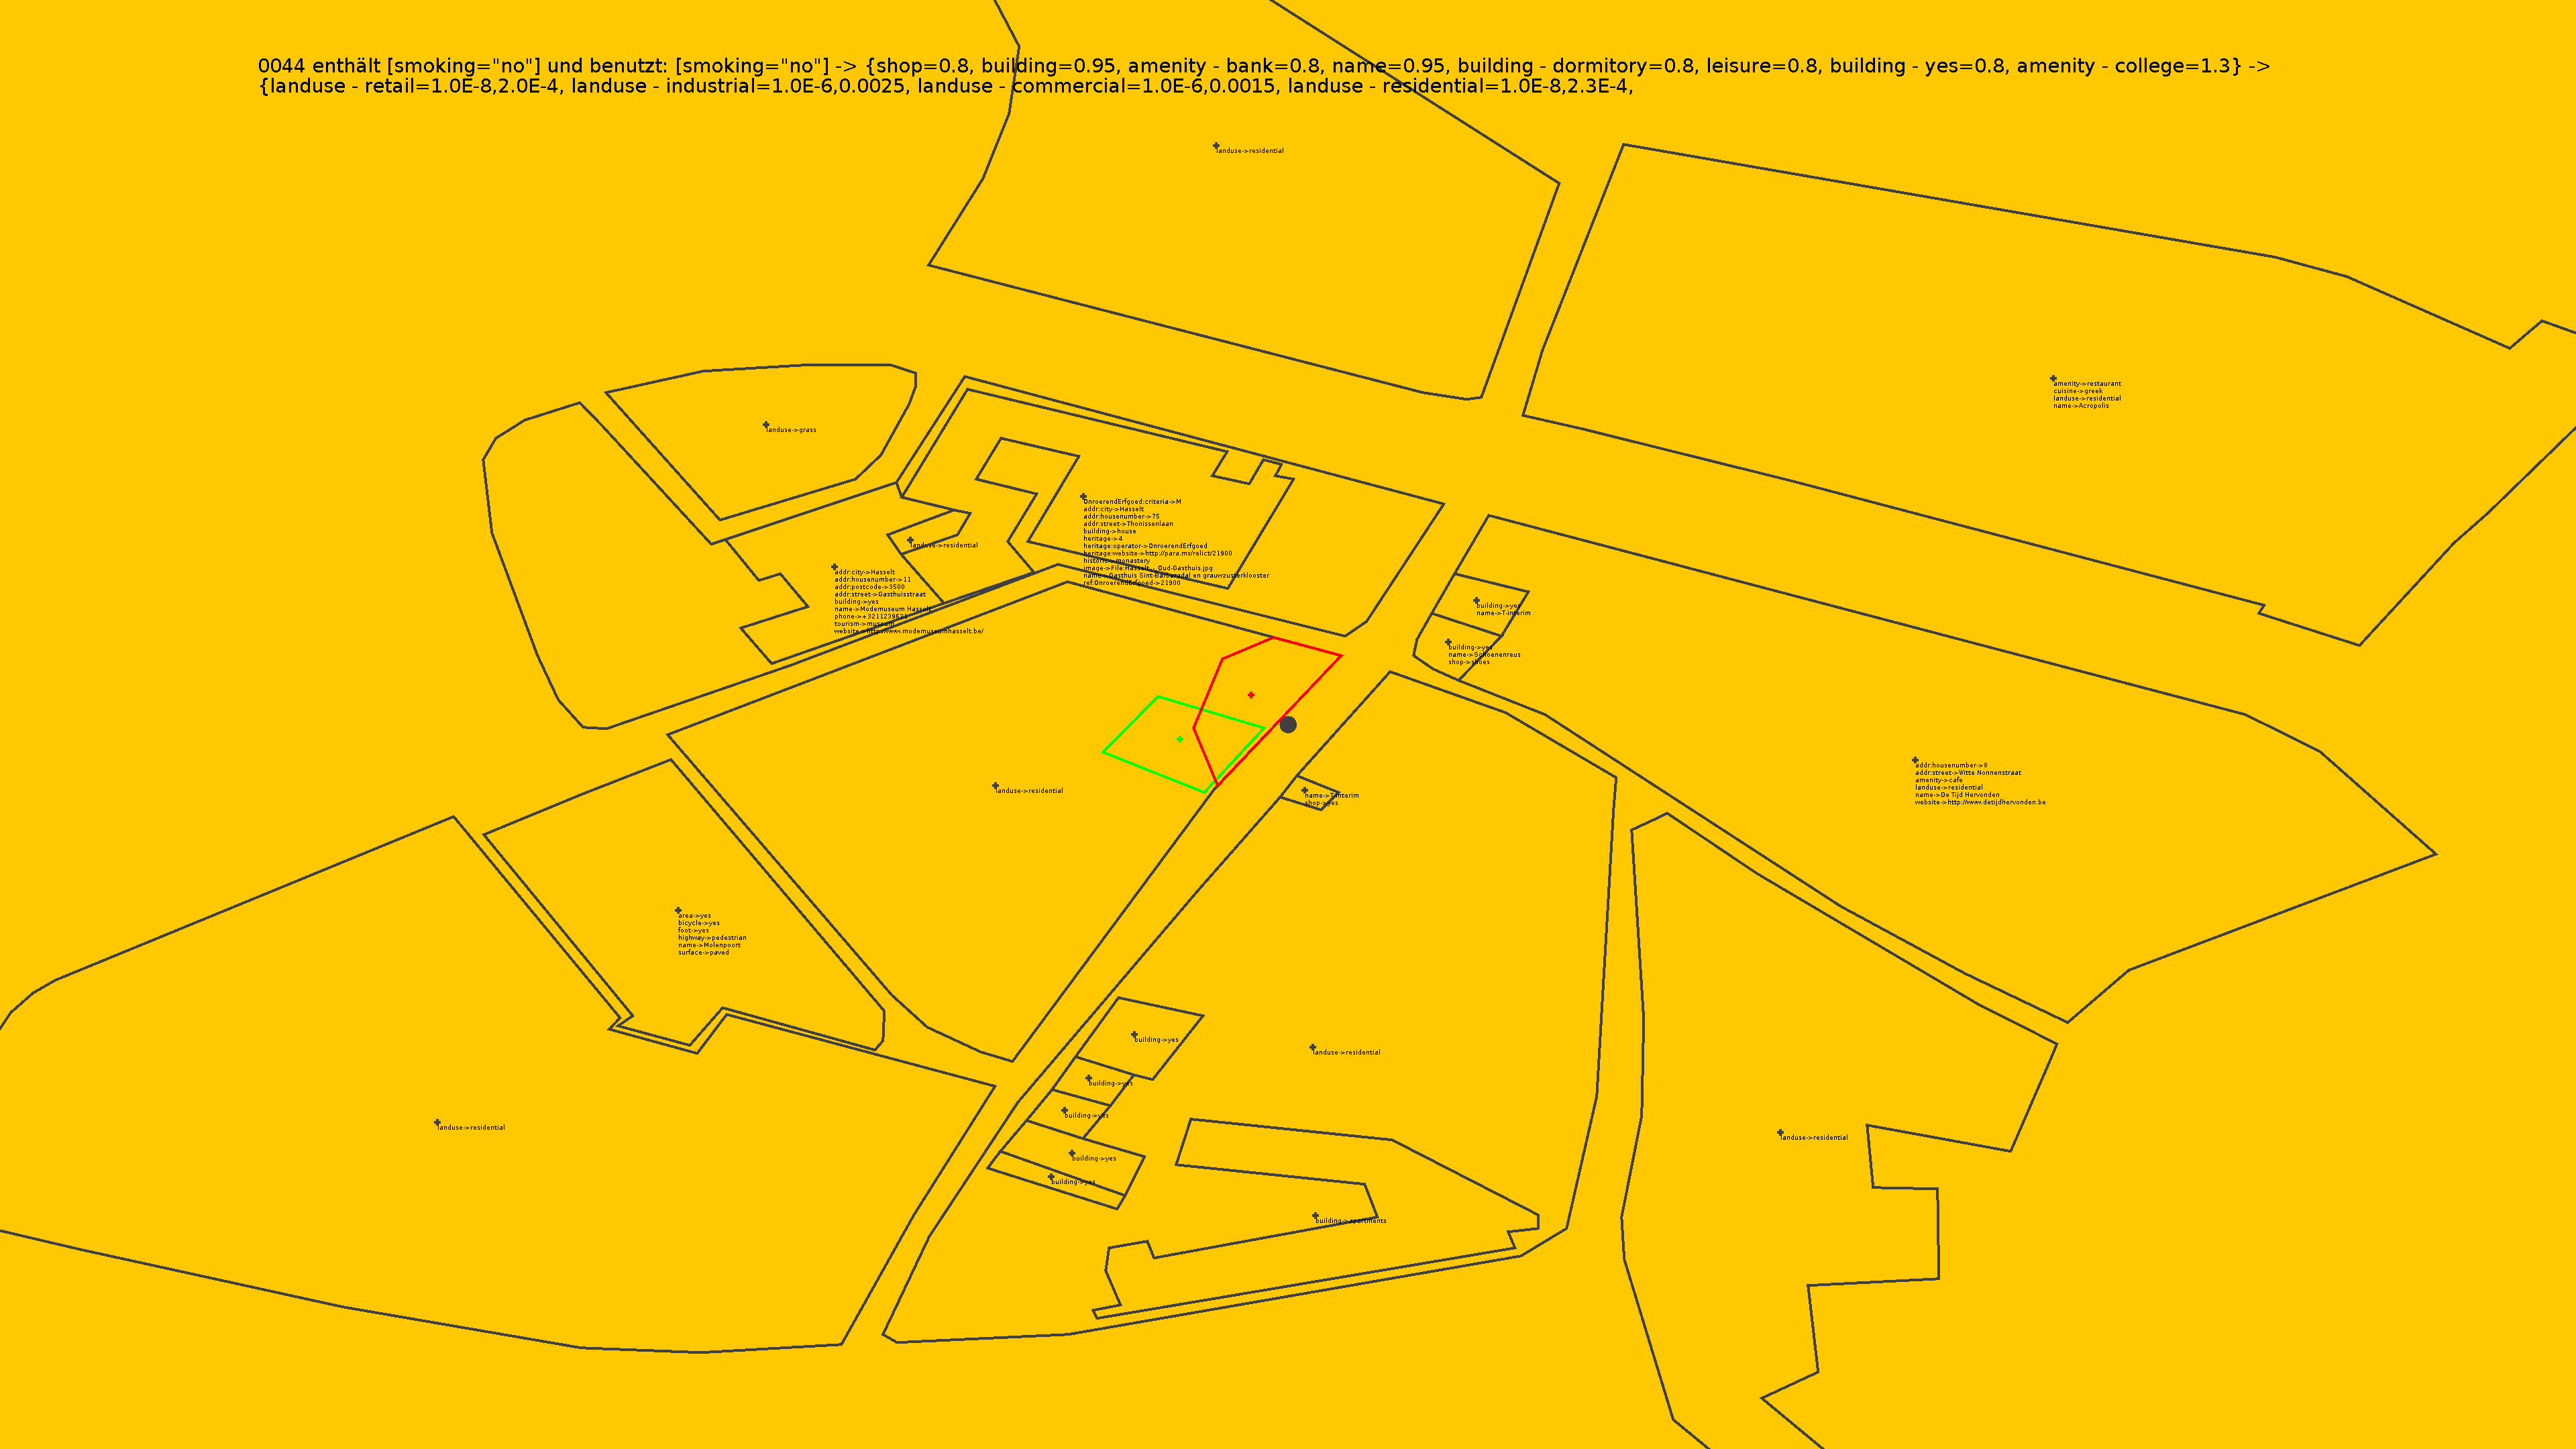
\includegraphics[width=\textwidth]{0044_big.png}}
\end{frame}


\begin{frame}
 \frametitle{Nicht geschafft}
  \Wider{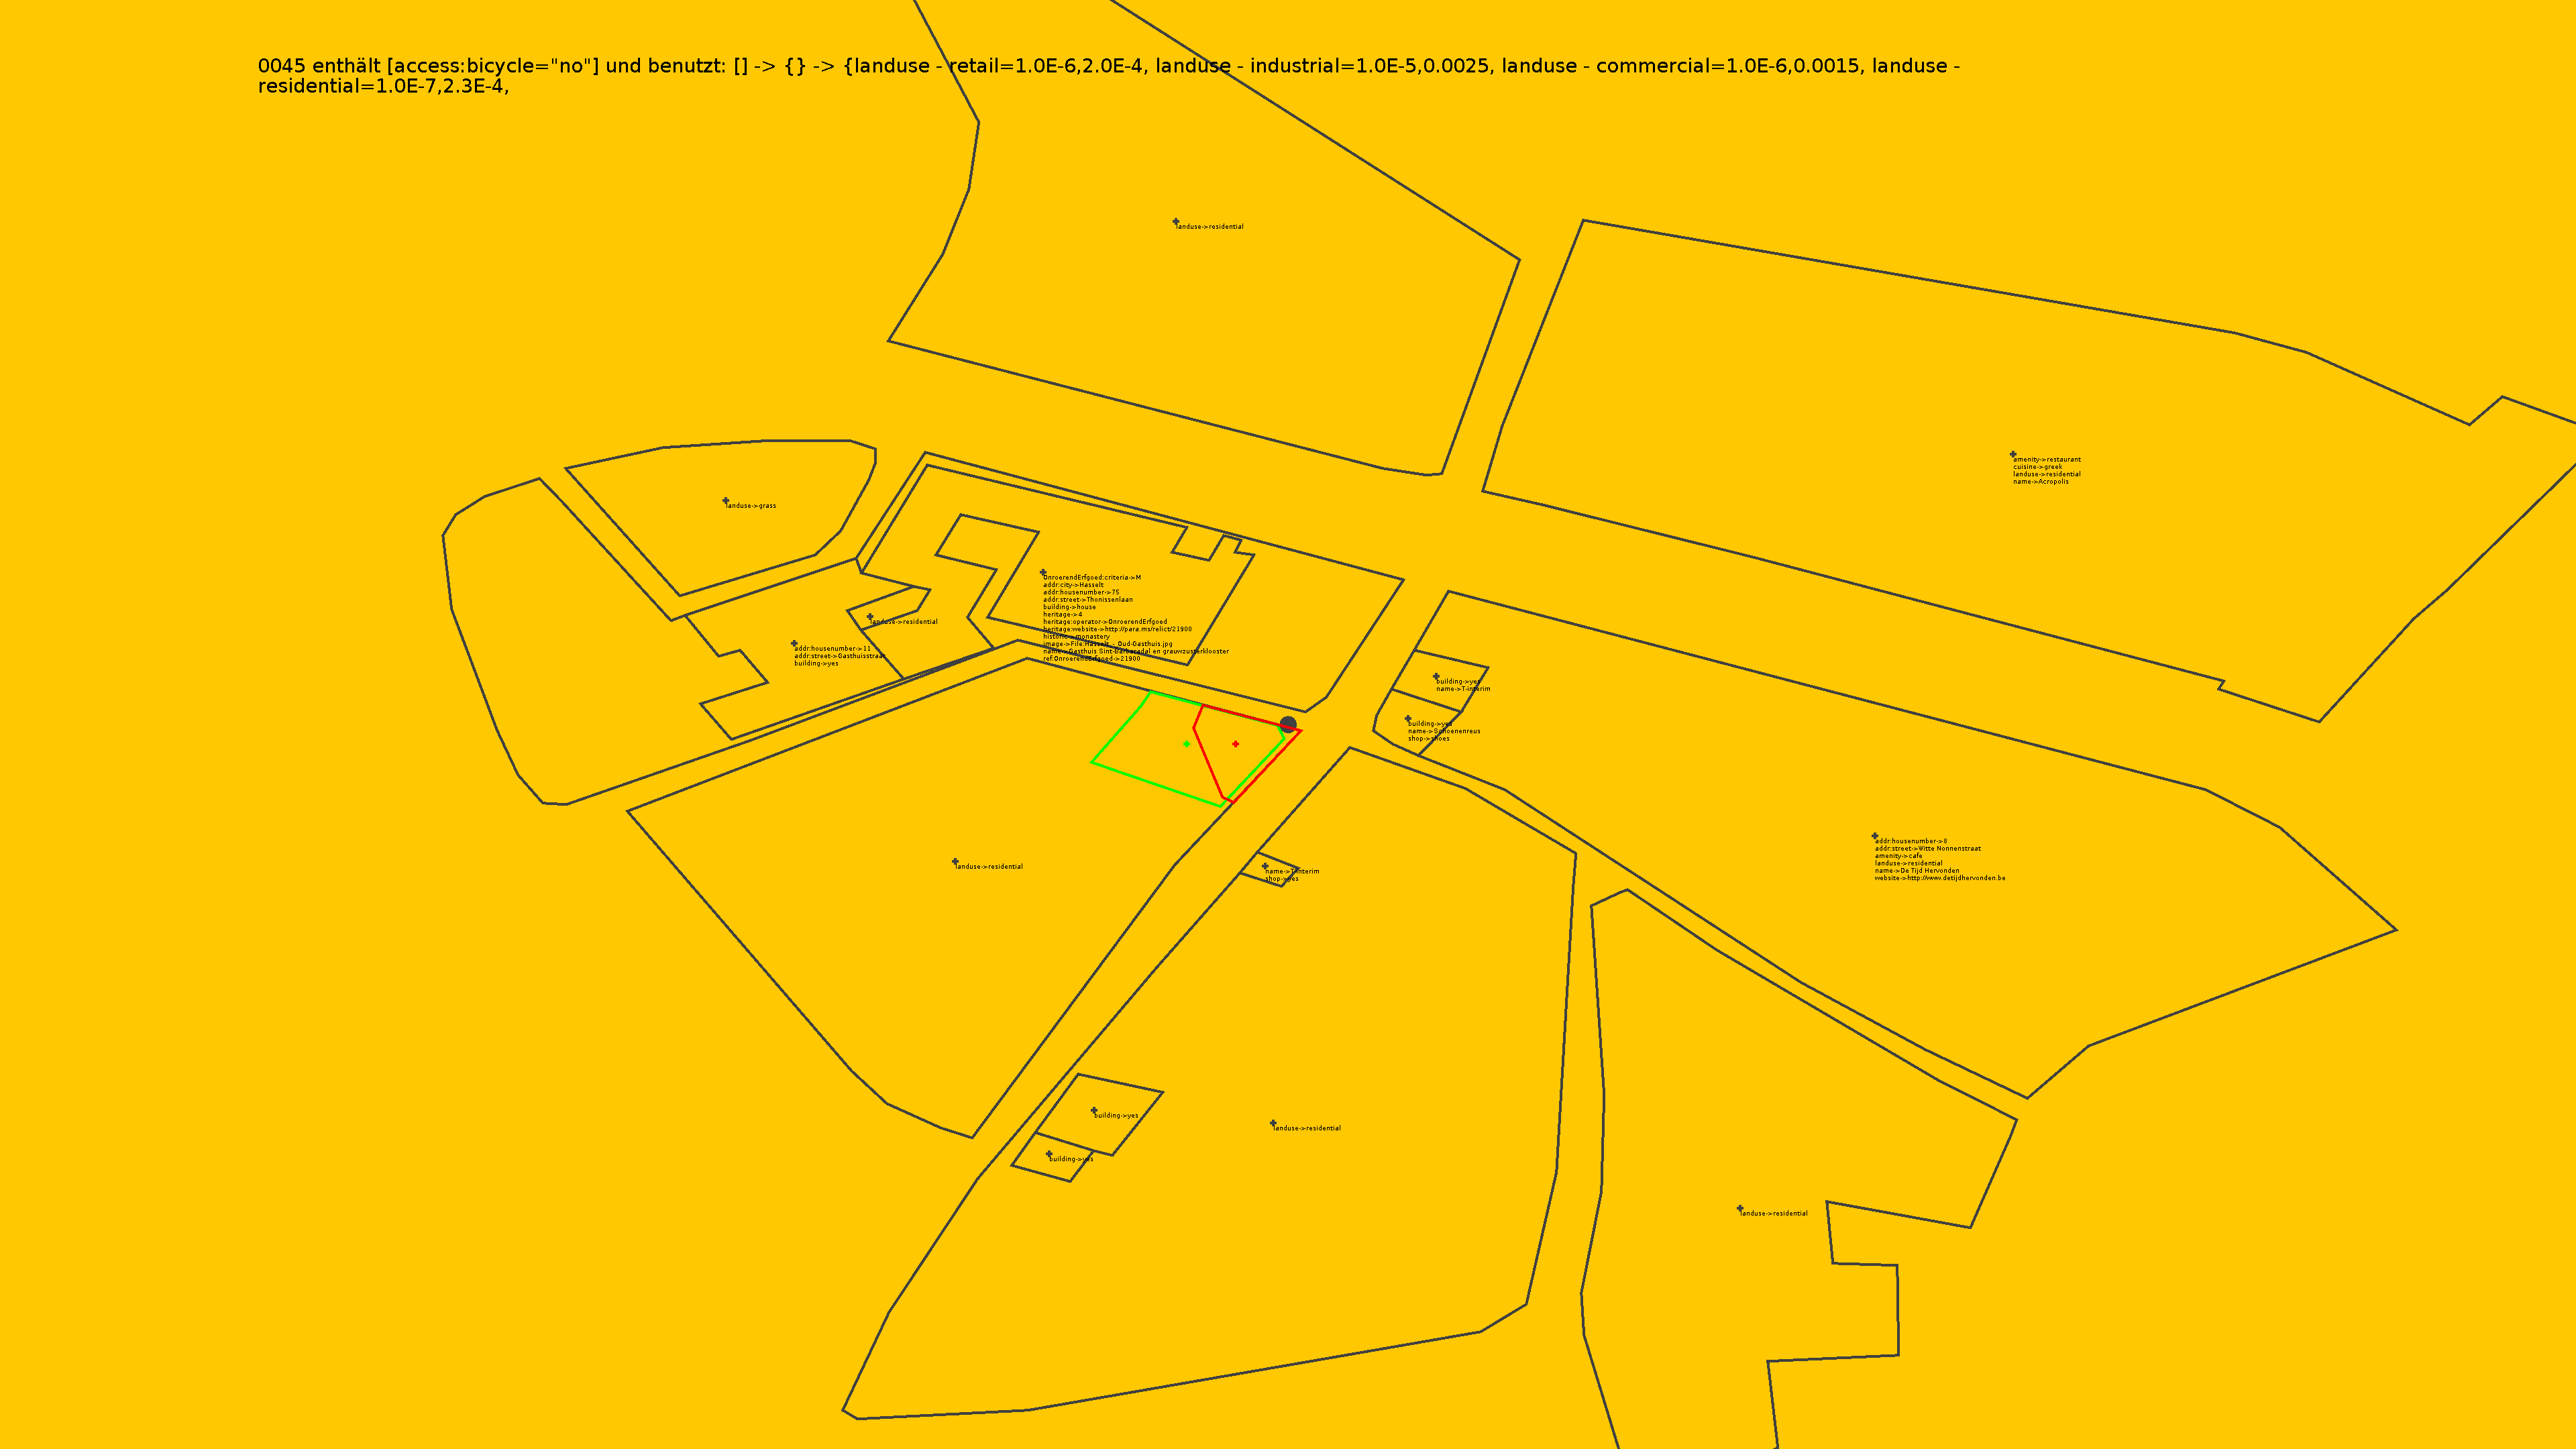
\includegraphics[width=\textwidth]{0045_big.png}}
\end{frame}


\begin{frame}
 \frametitle{Nicht geschafft}
  \Wider{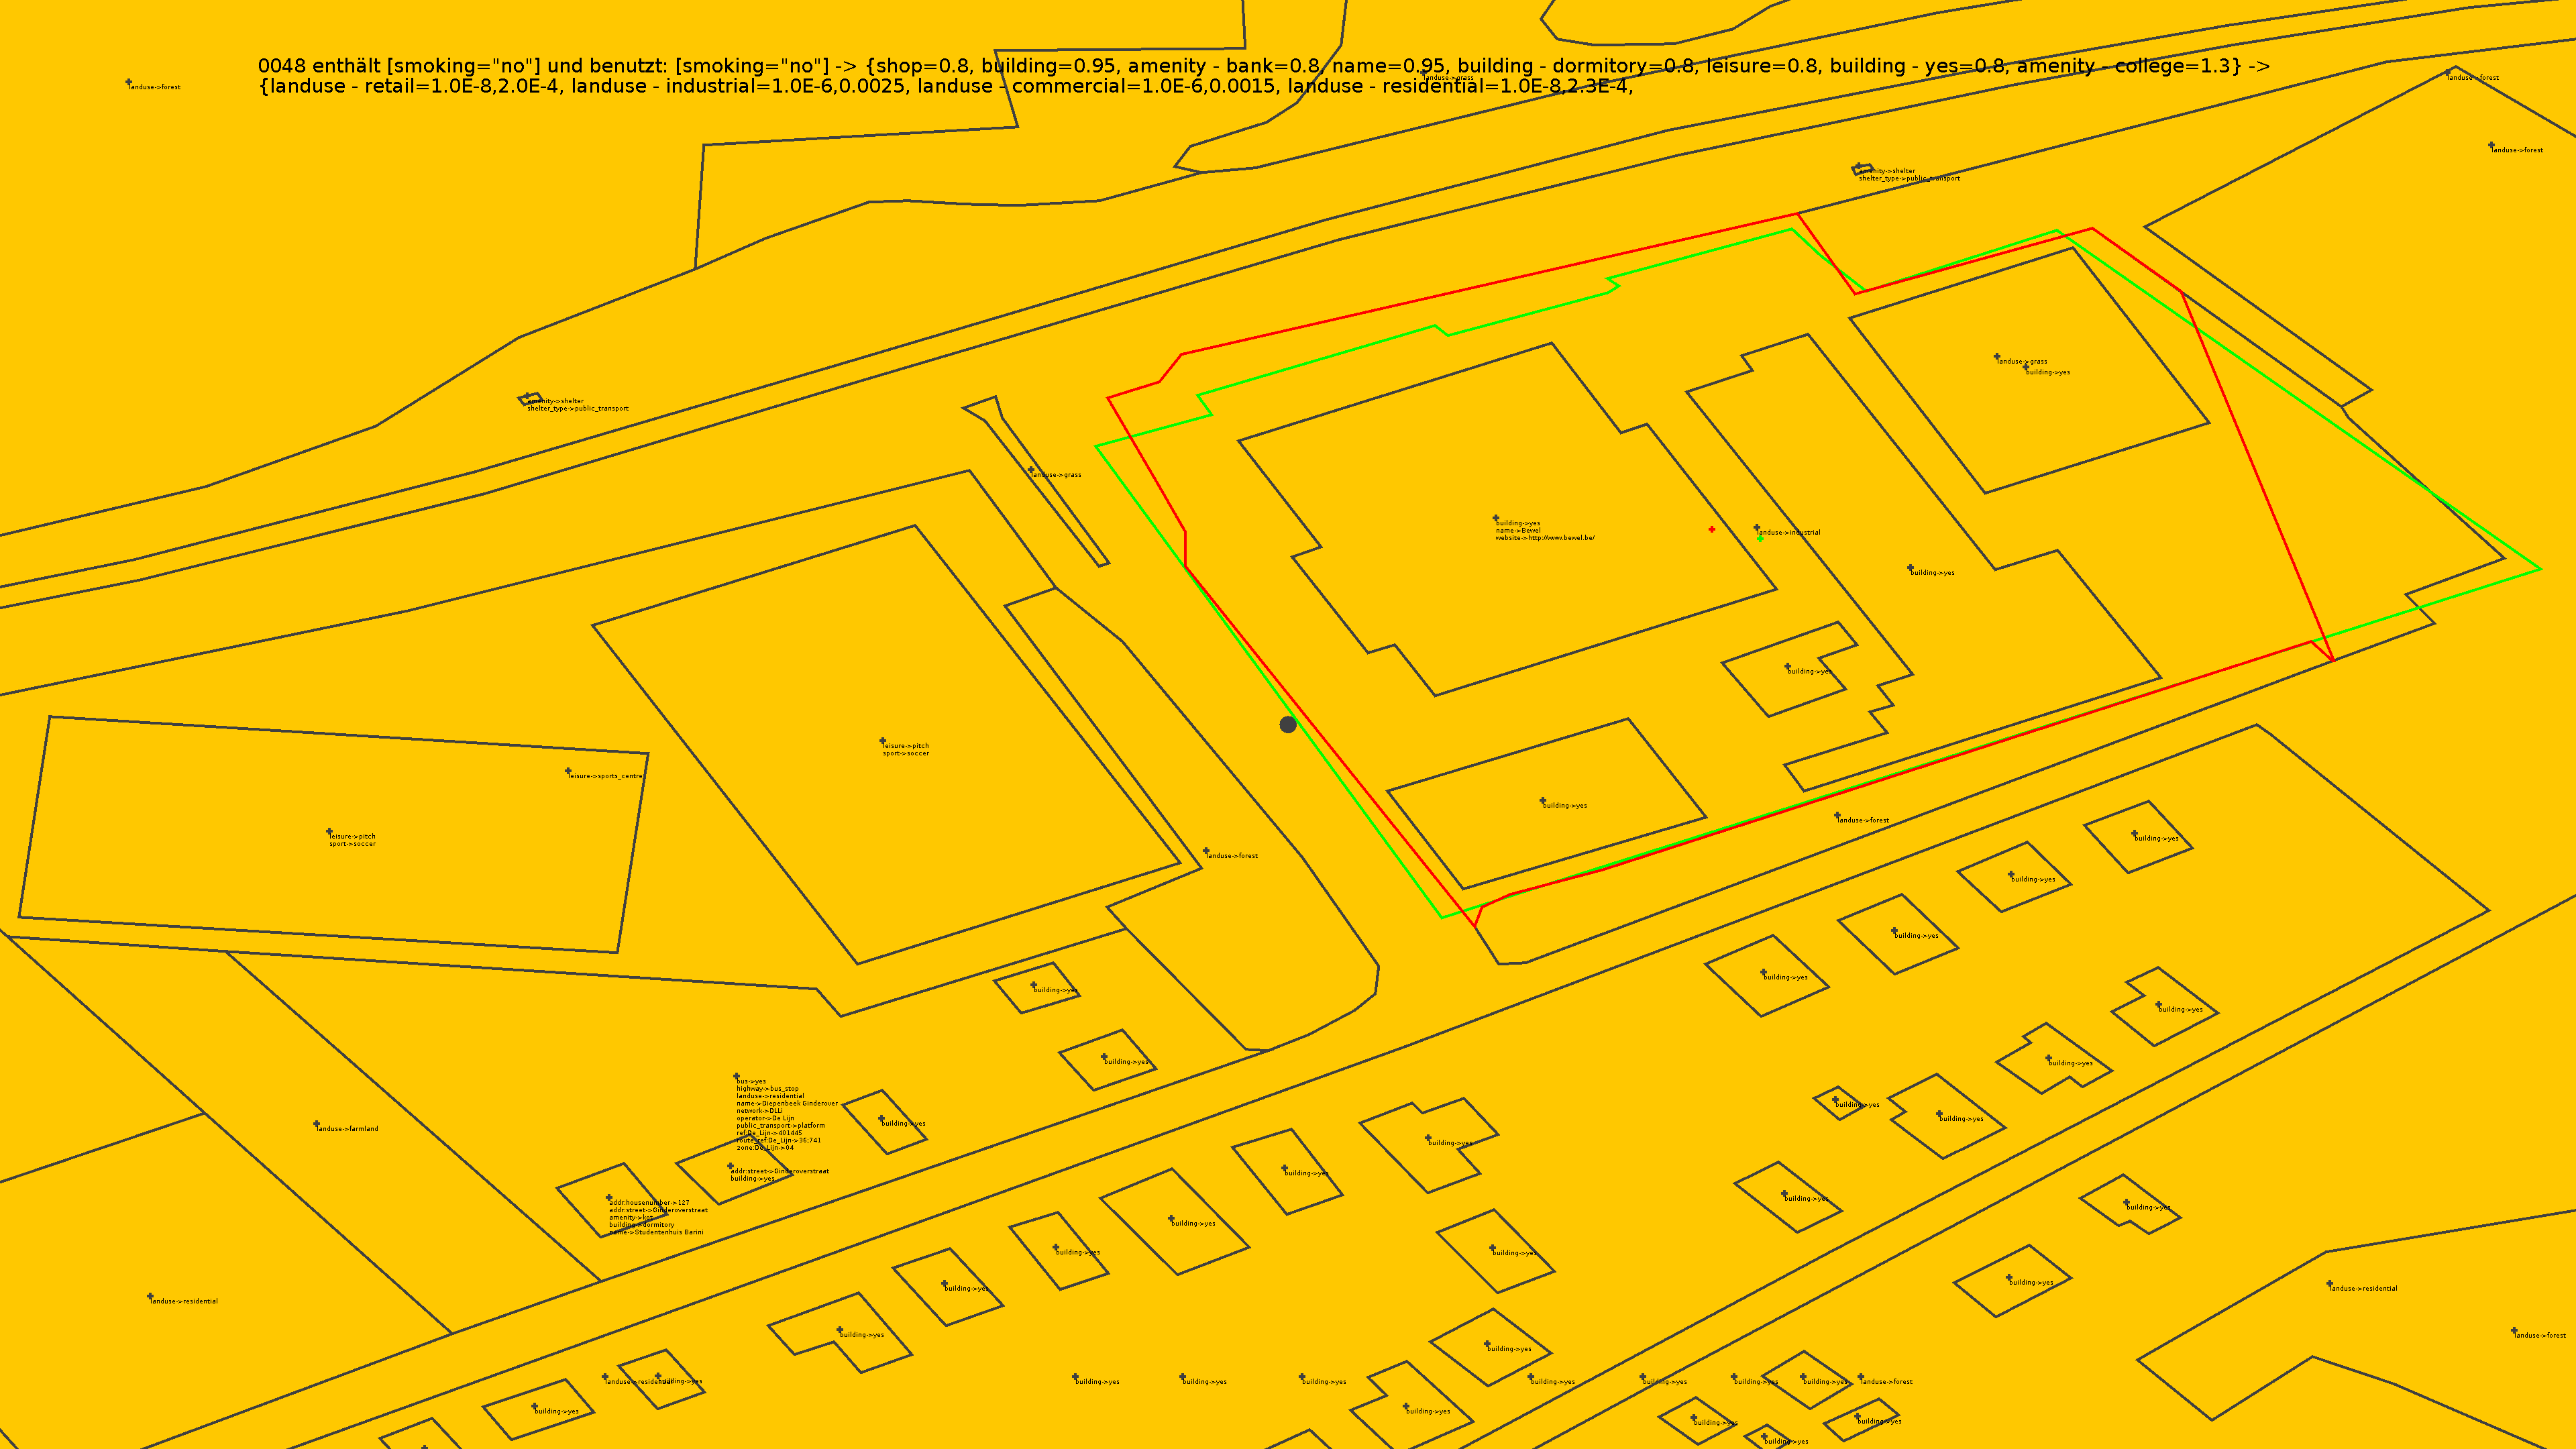
\includegraphics[width=\textwidth]{0048_big.png}}
\end{frame}


\begin{frame}
 \frametitle{Nicht geschafft}
  \Wider{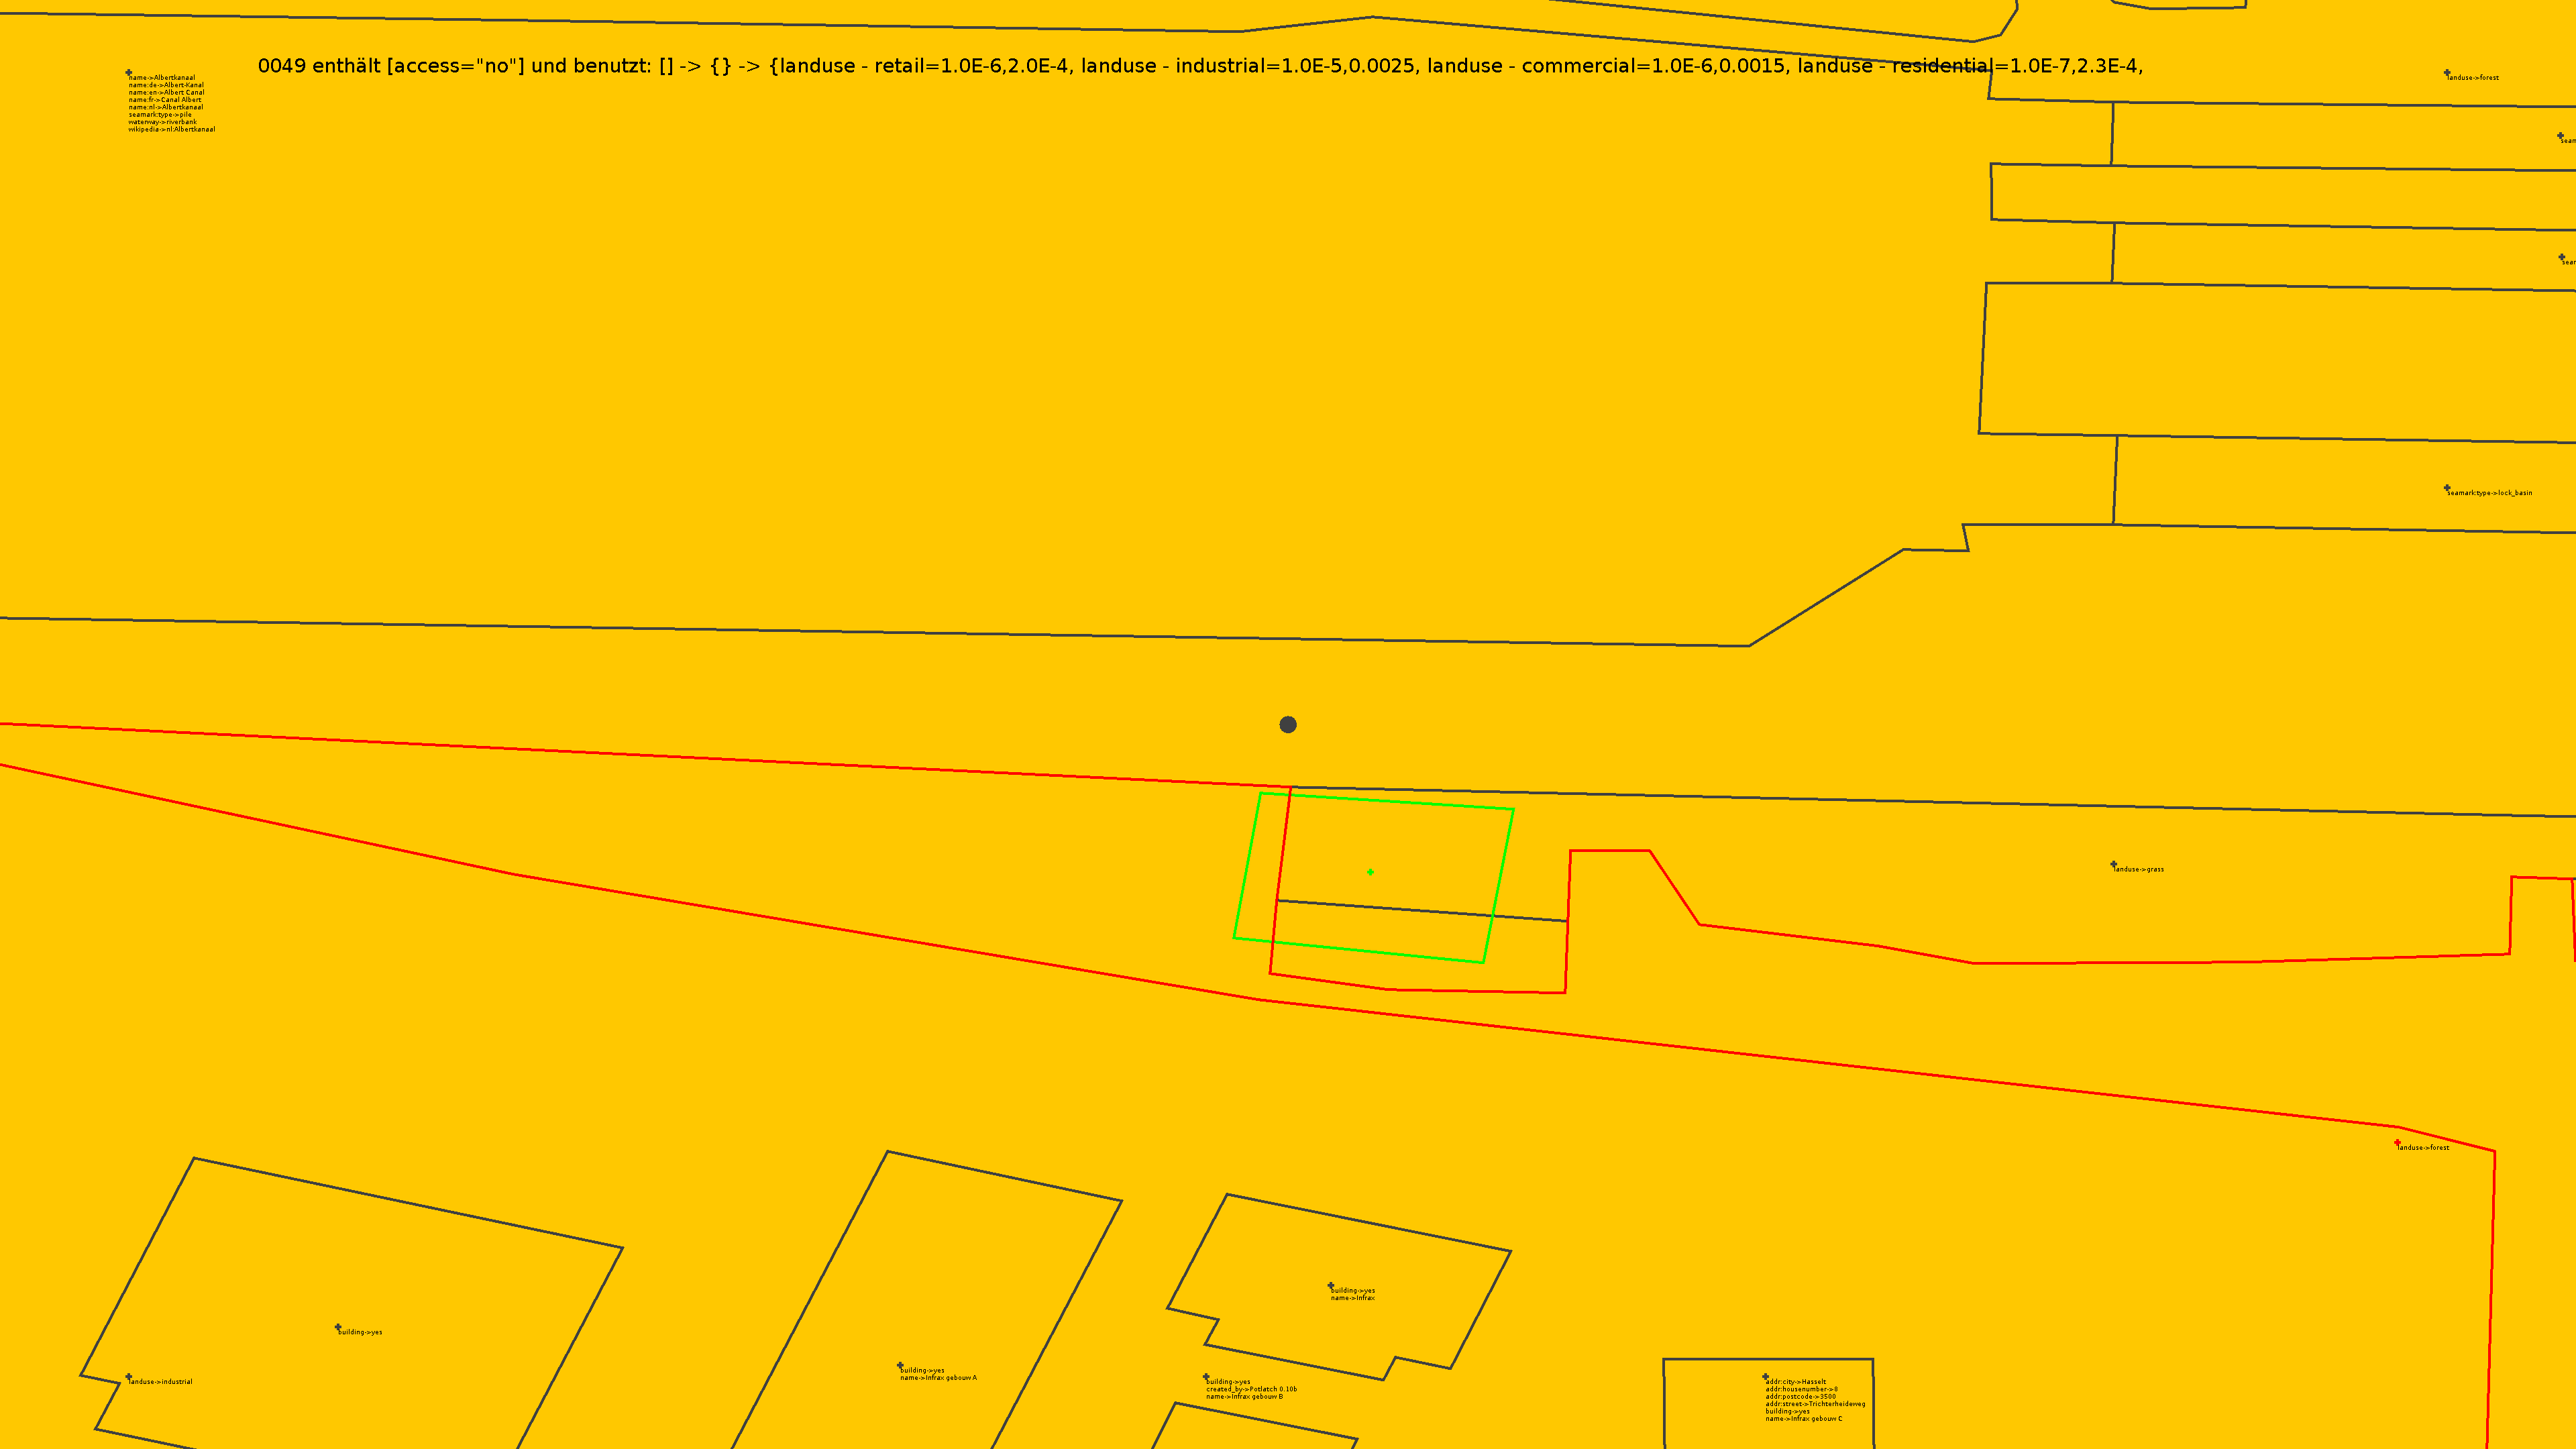
\includegraphics[width=\textwidth]{0049_big.png}}
\end{frame}


\begin{frame}
 \frametitle{Nicht geschafft}
  \Wider{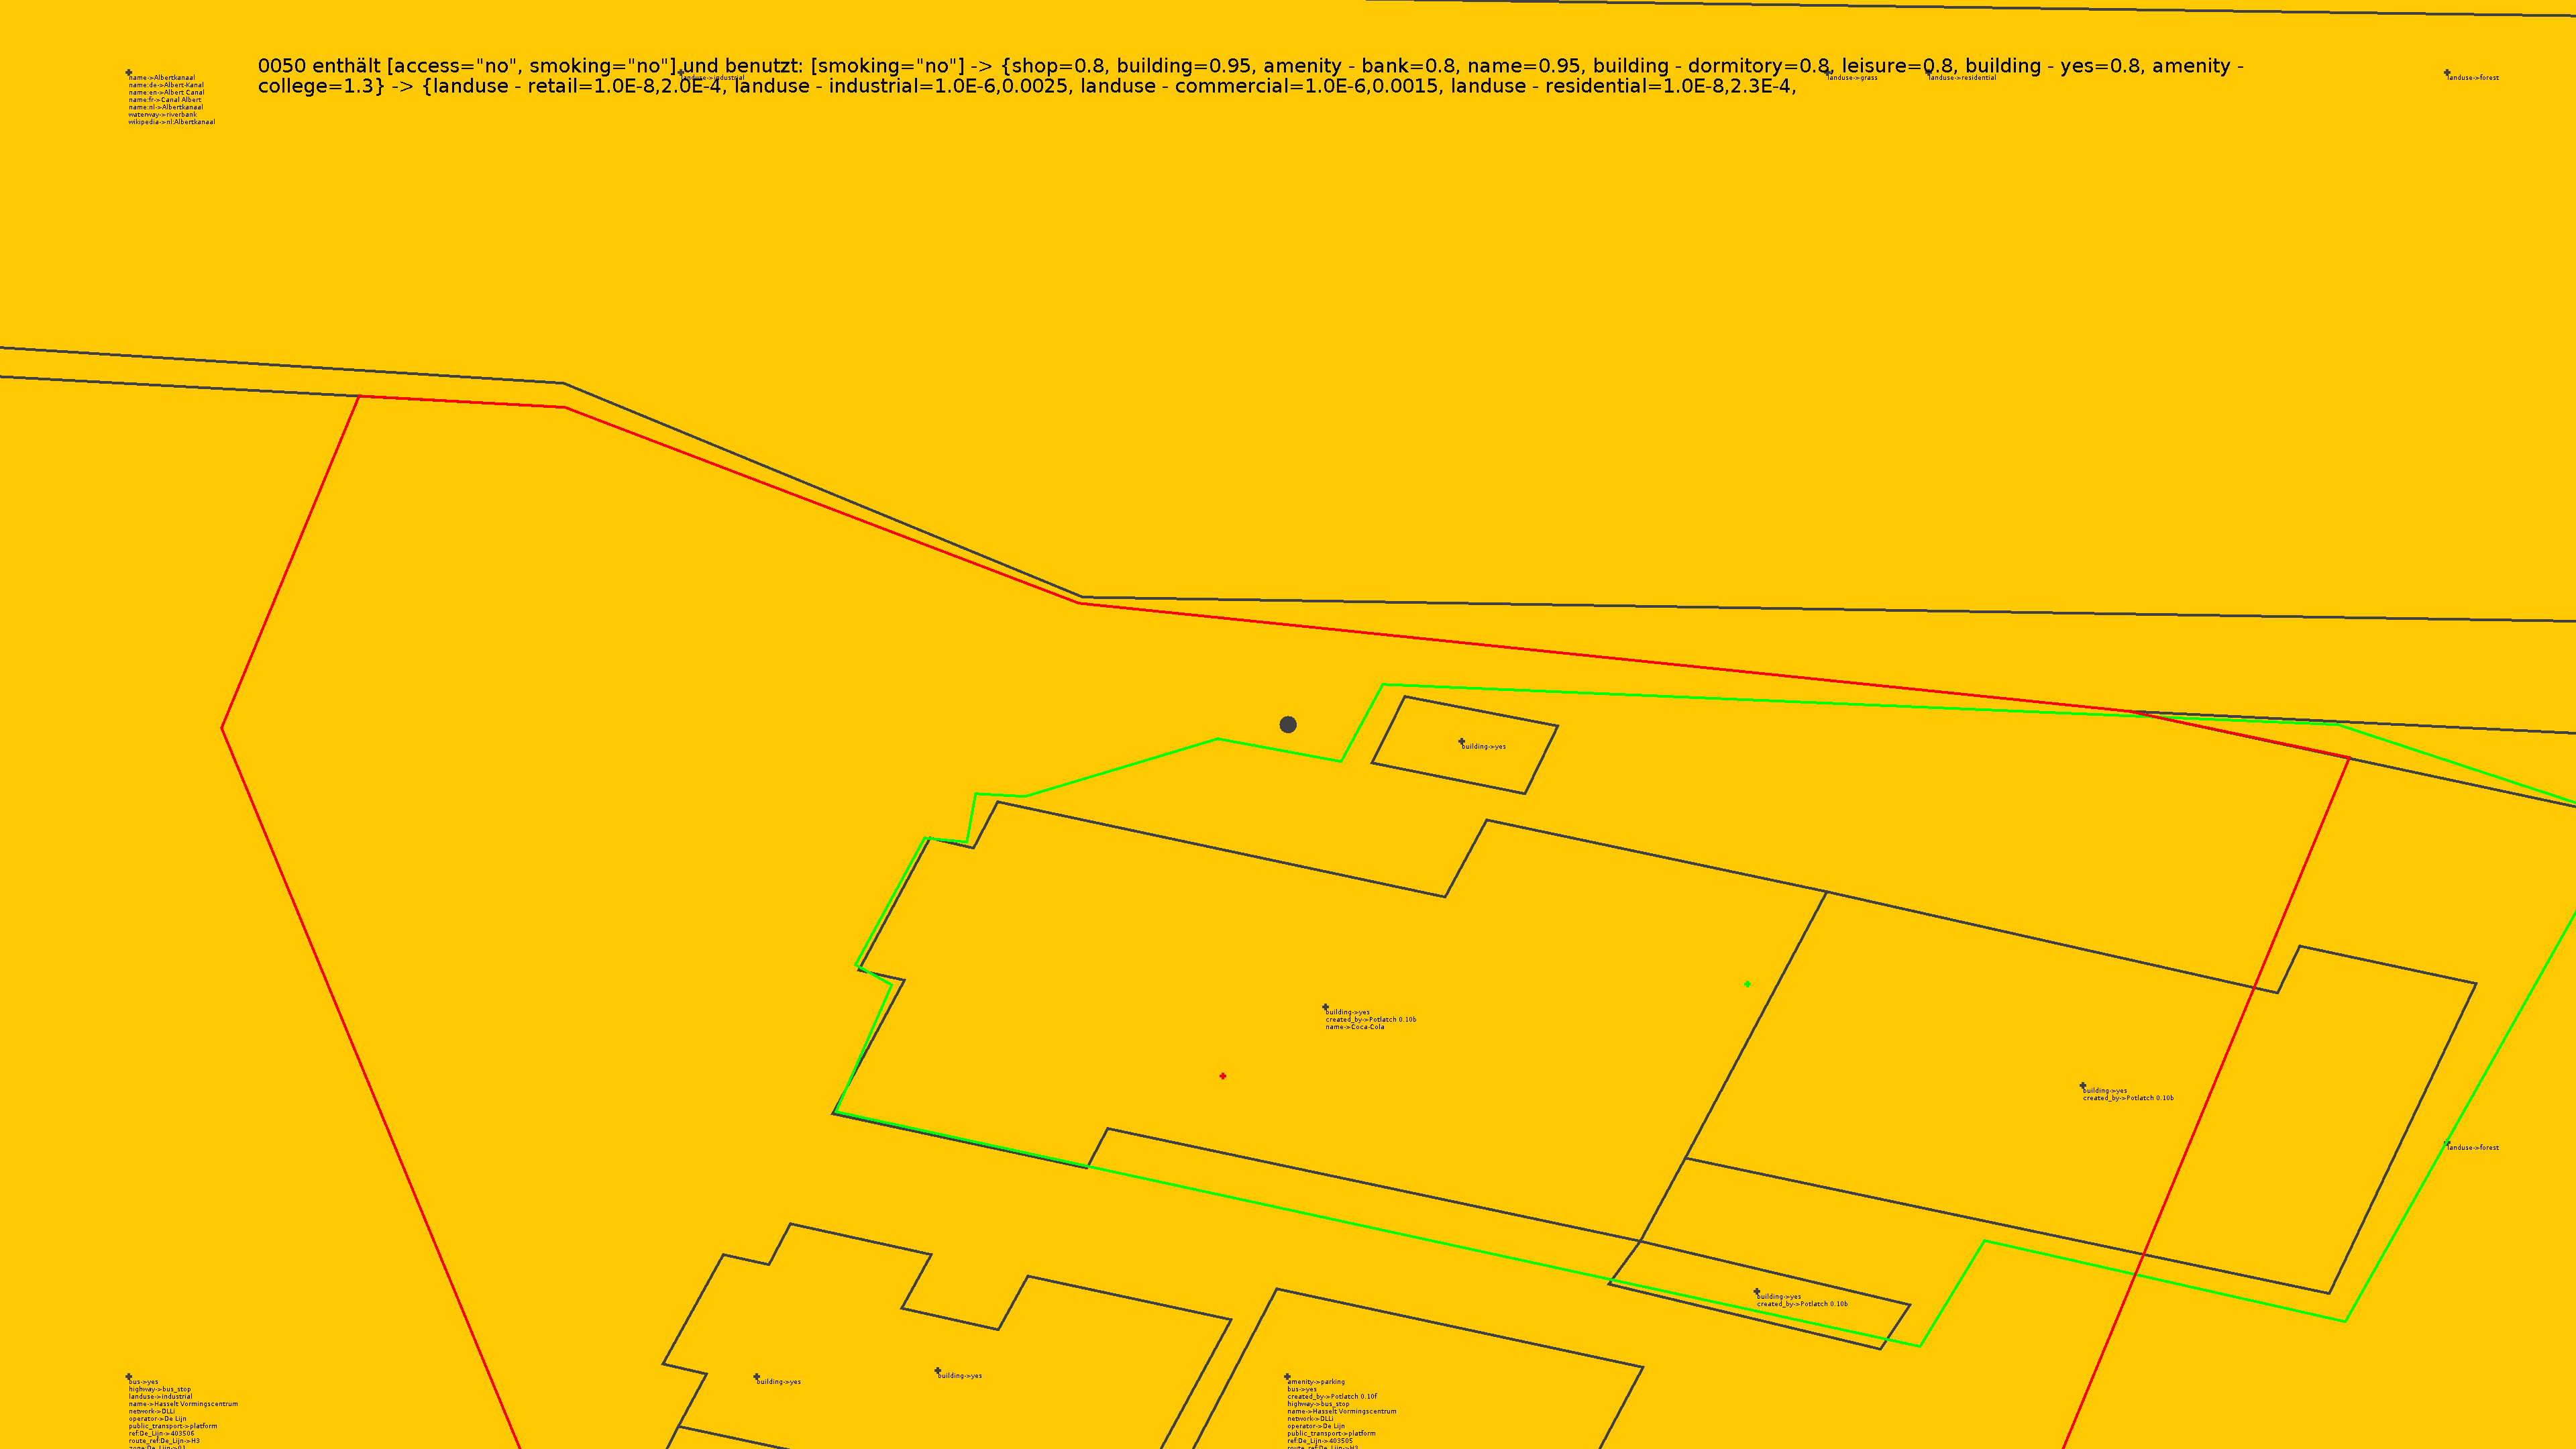
\includegraphics[width=\textwidth]{0050_big.png}}
\end{frame}


\begin{frame}
 \frametitle{Nicht geschafft}
  \Wider{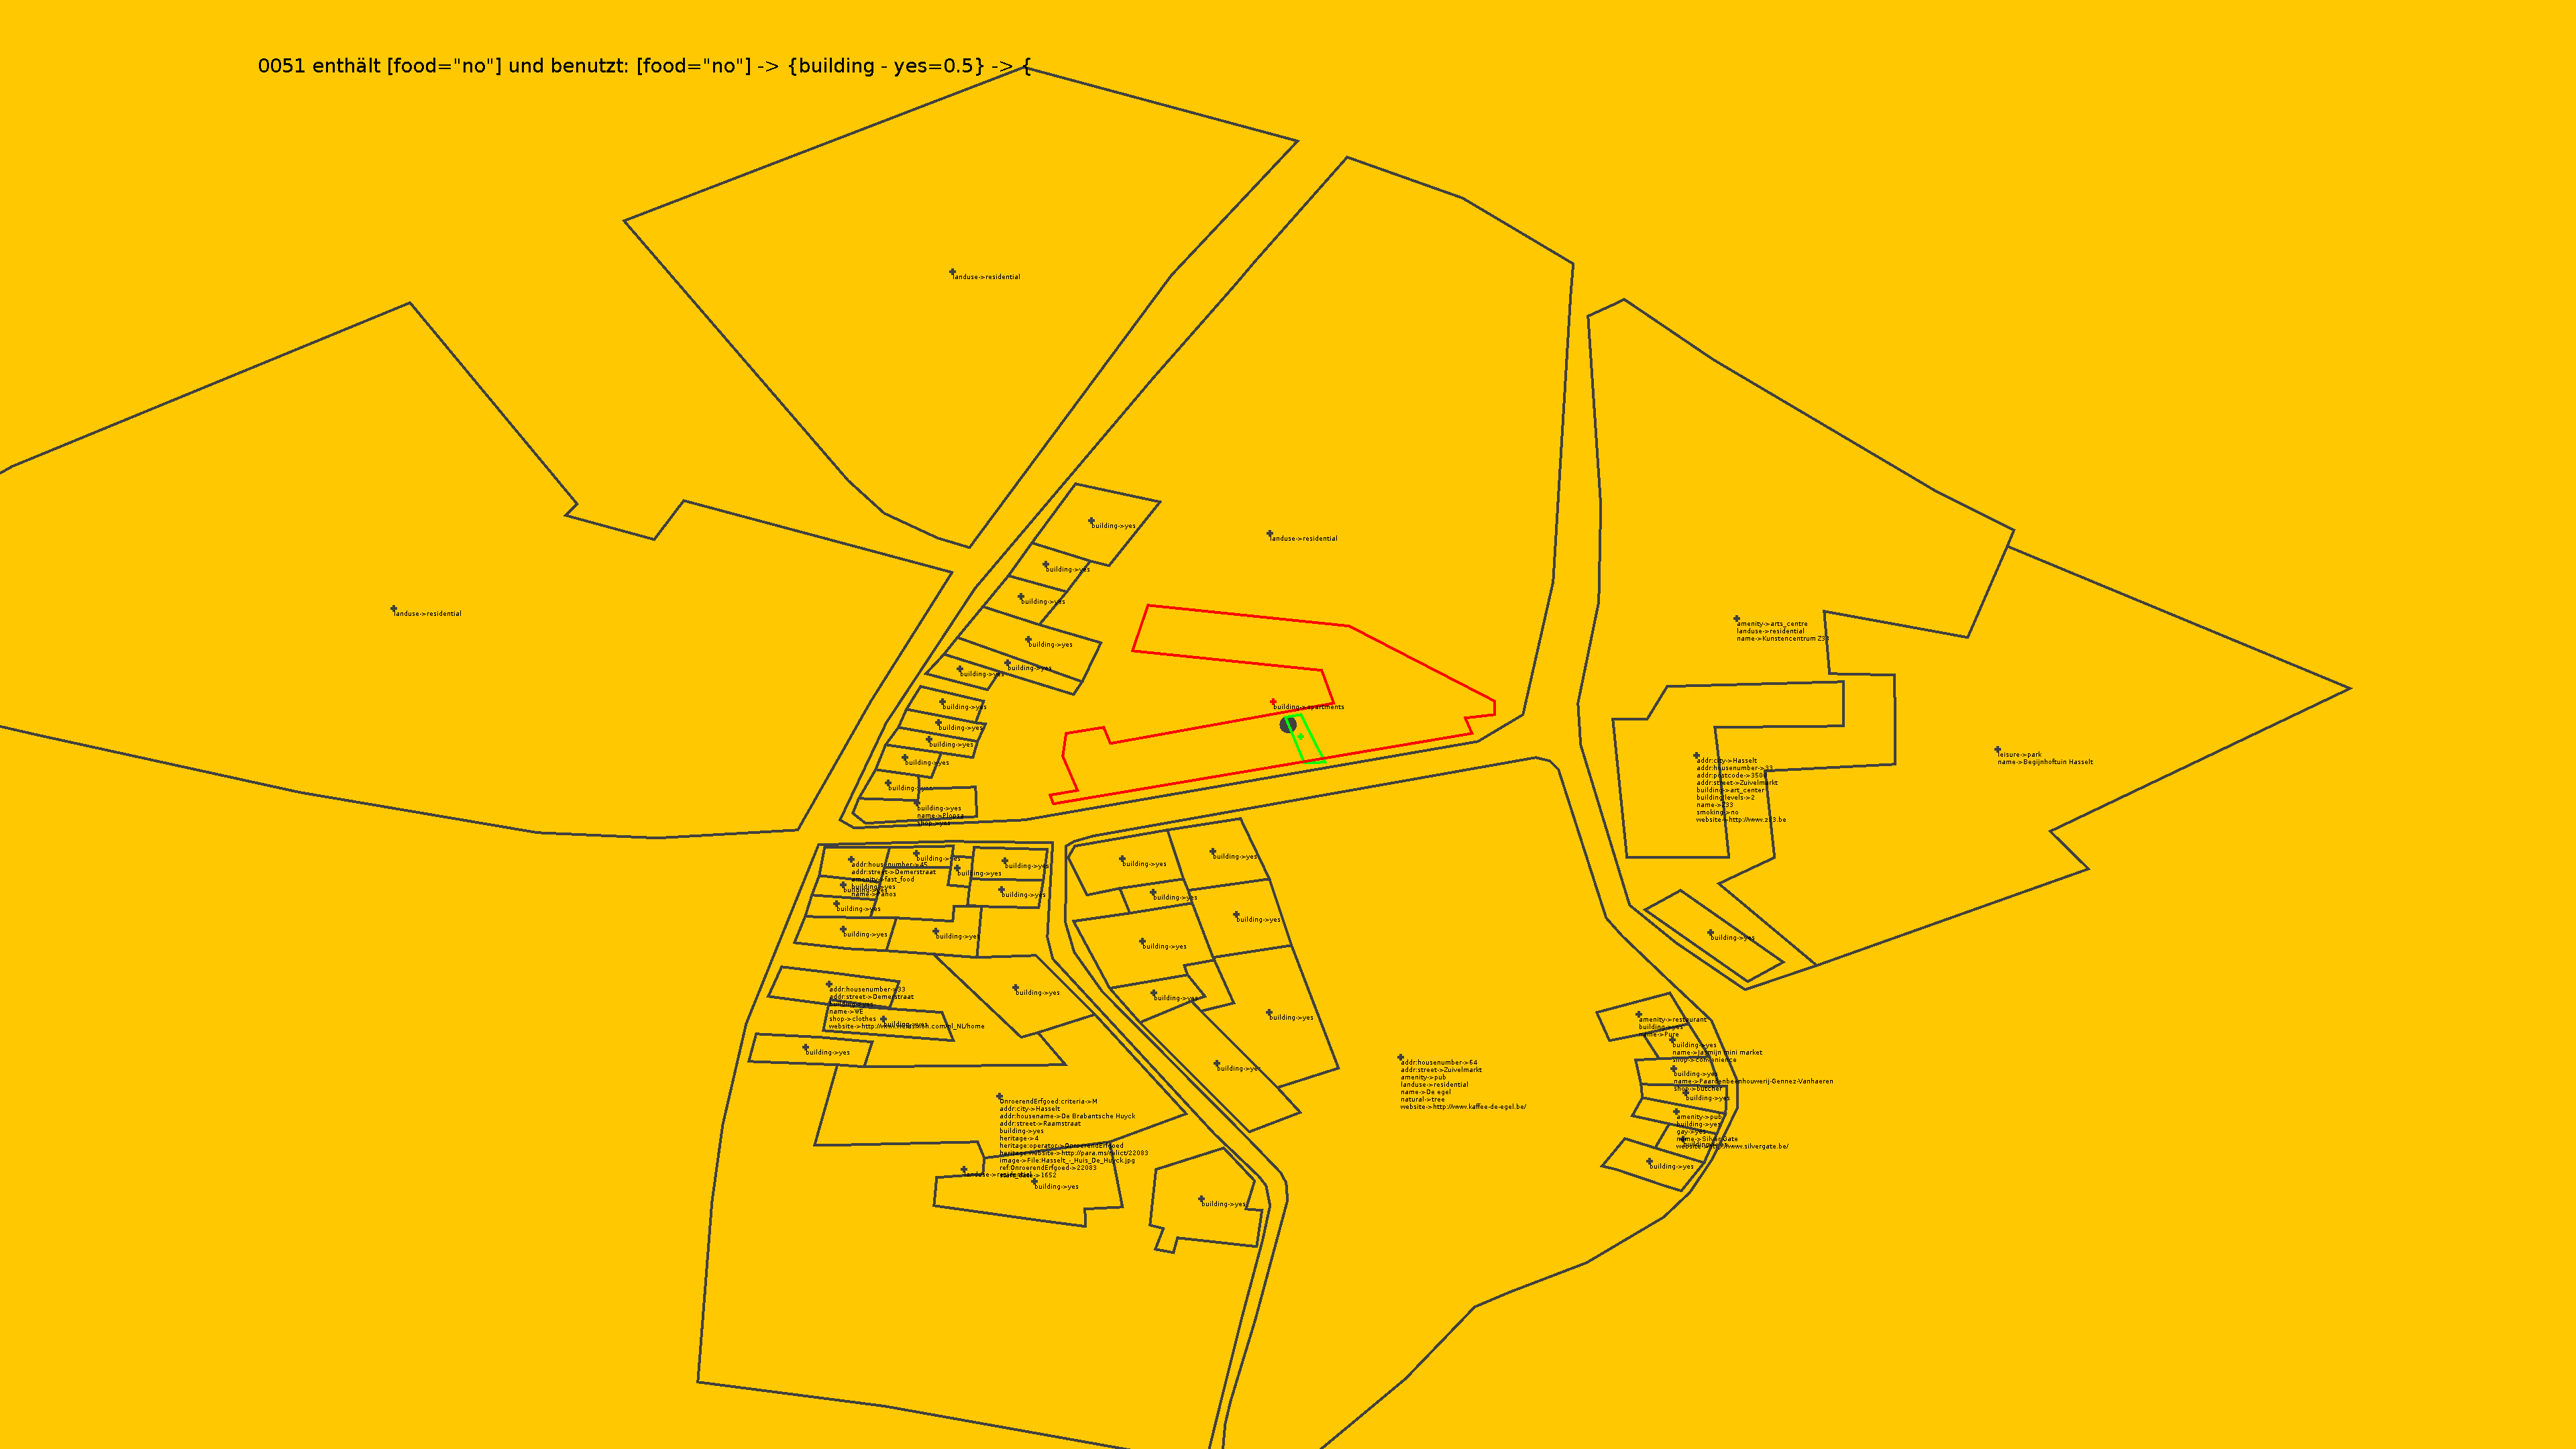
\includegraphics[width=\textwidth]{0051_big.png}}
\end{frame}


\begin{frame}
 \frametitle{Nicht geschafft}
  \Wider{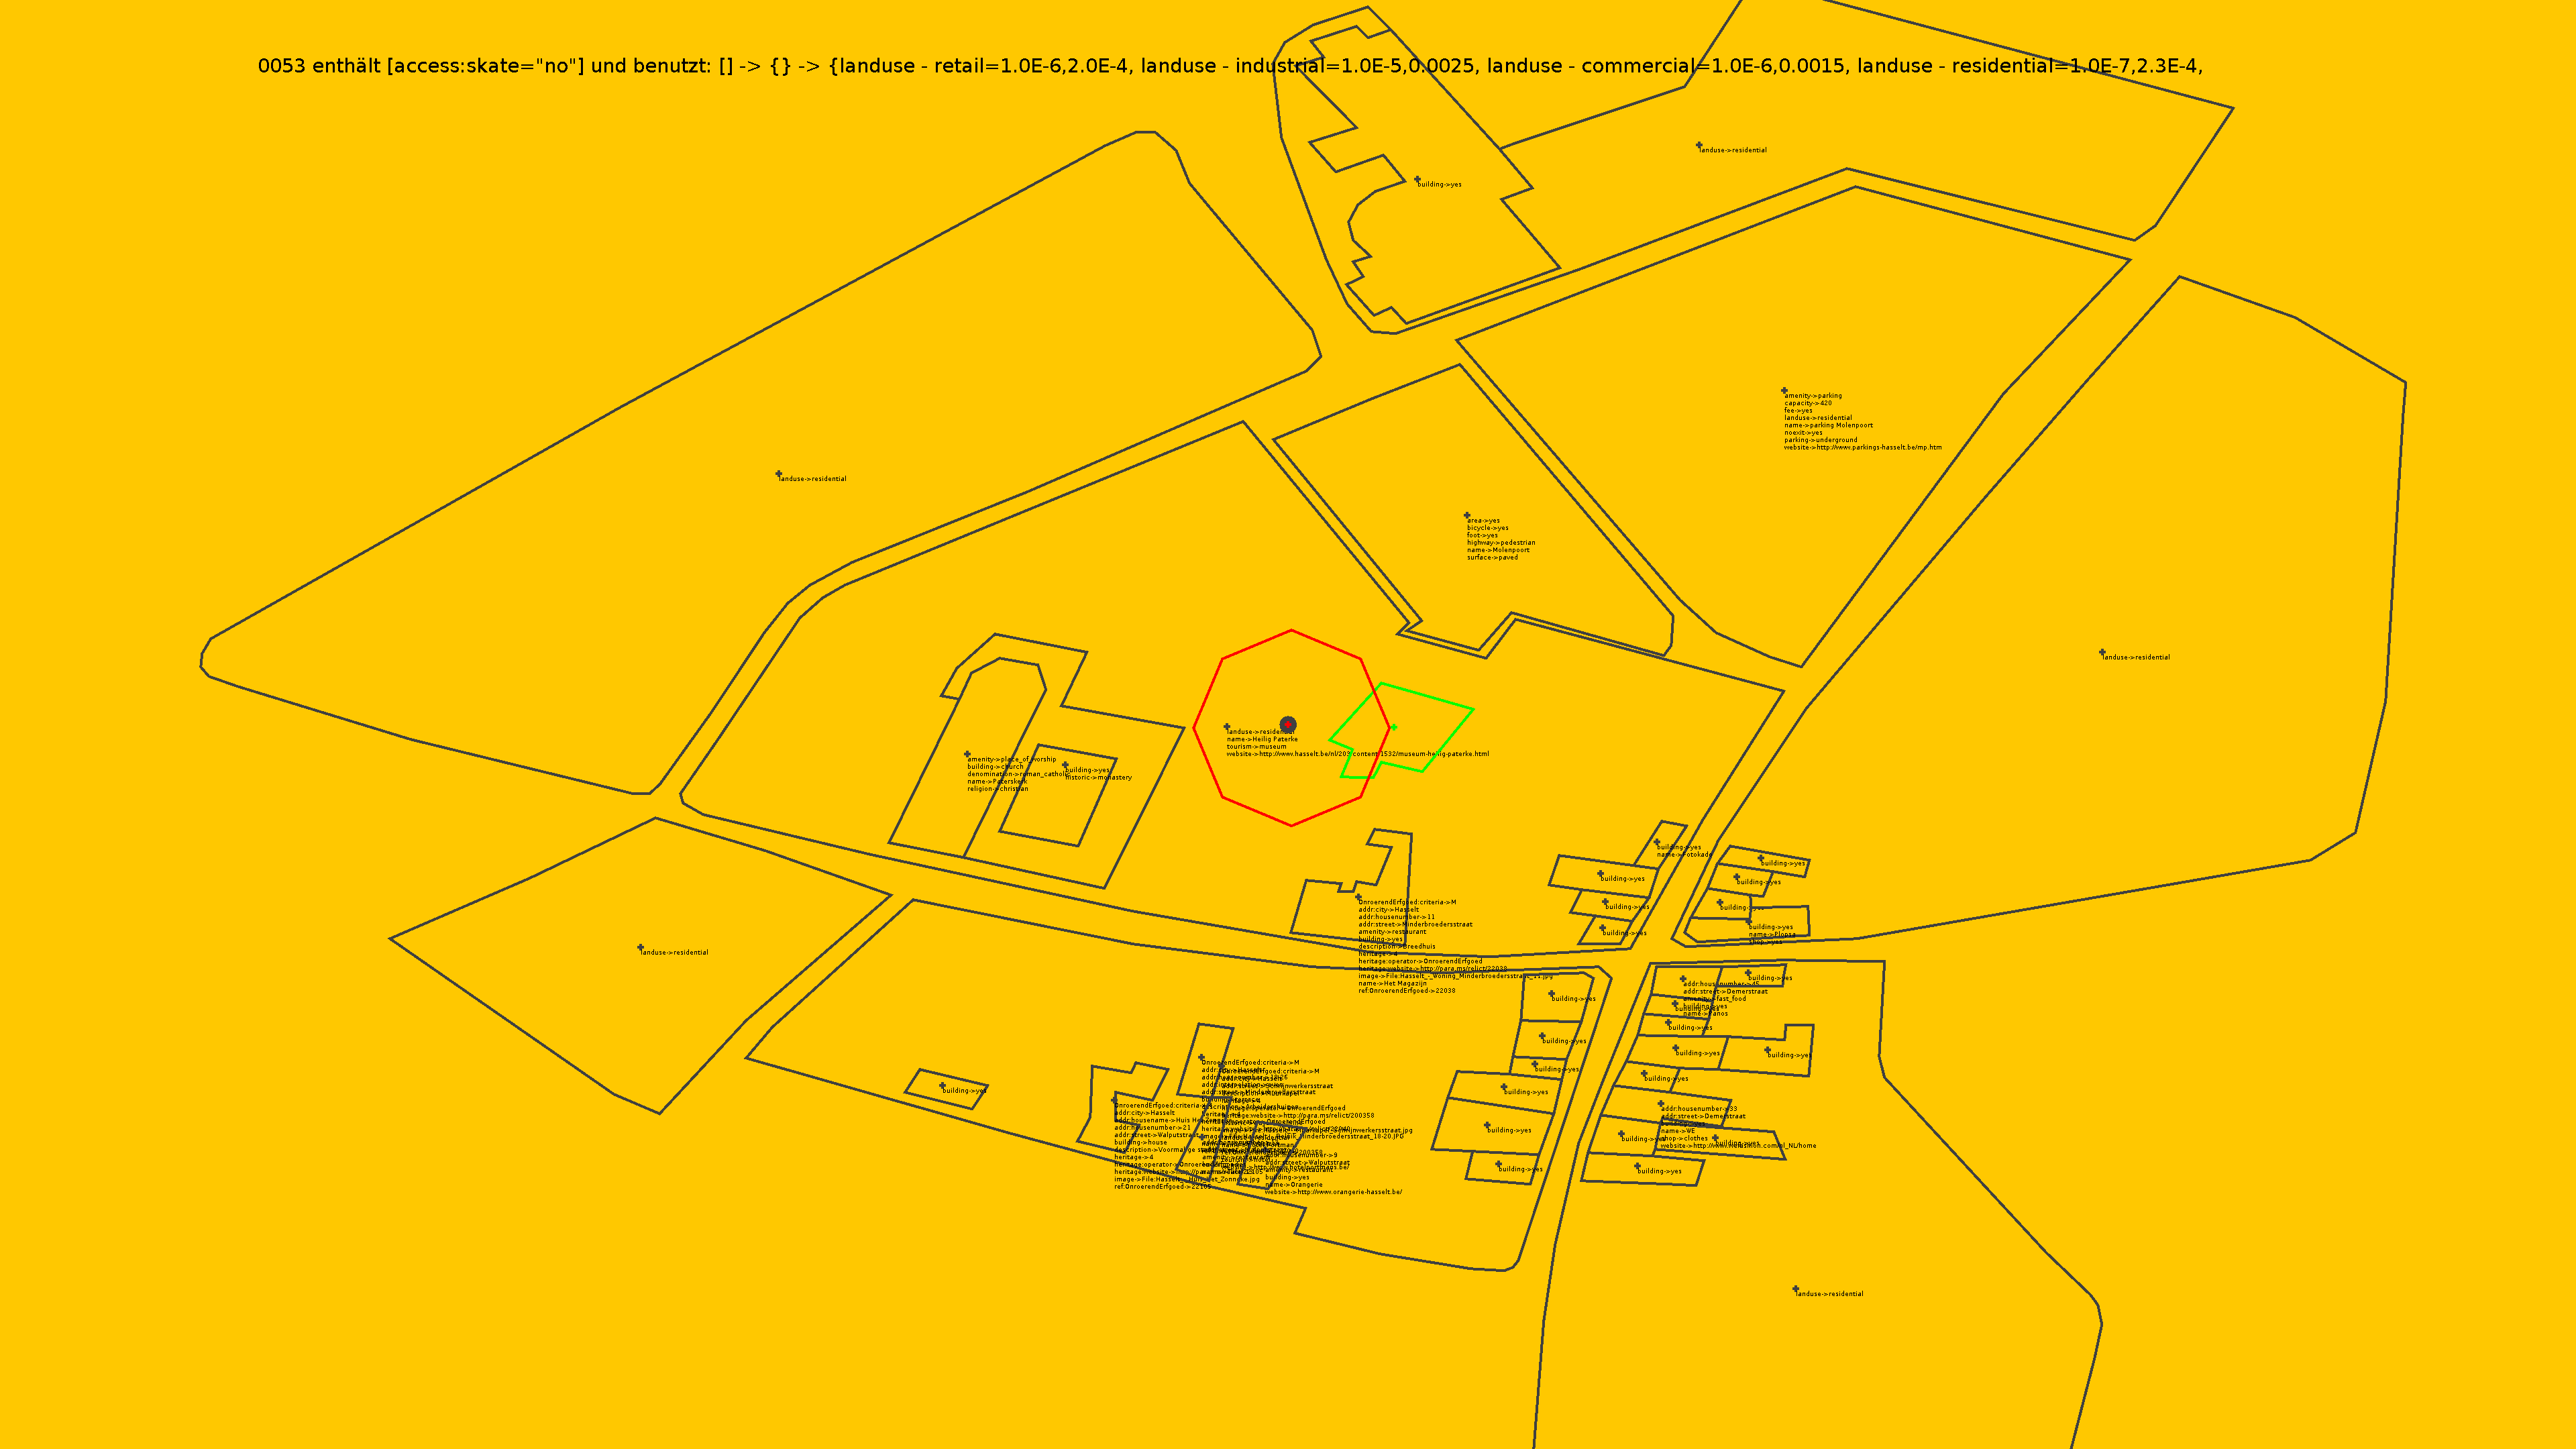
\includegraphics[width=\textwidth]{0053_big.png}}
\end{frame}


\begin{frame}
 \frametitle{Nicht geschafft}
  \Wider{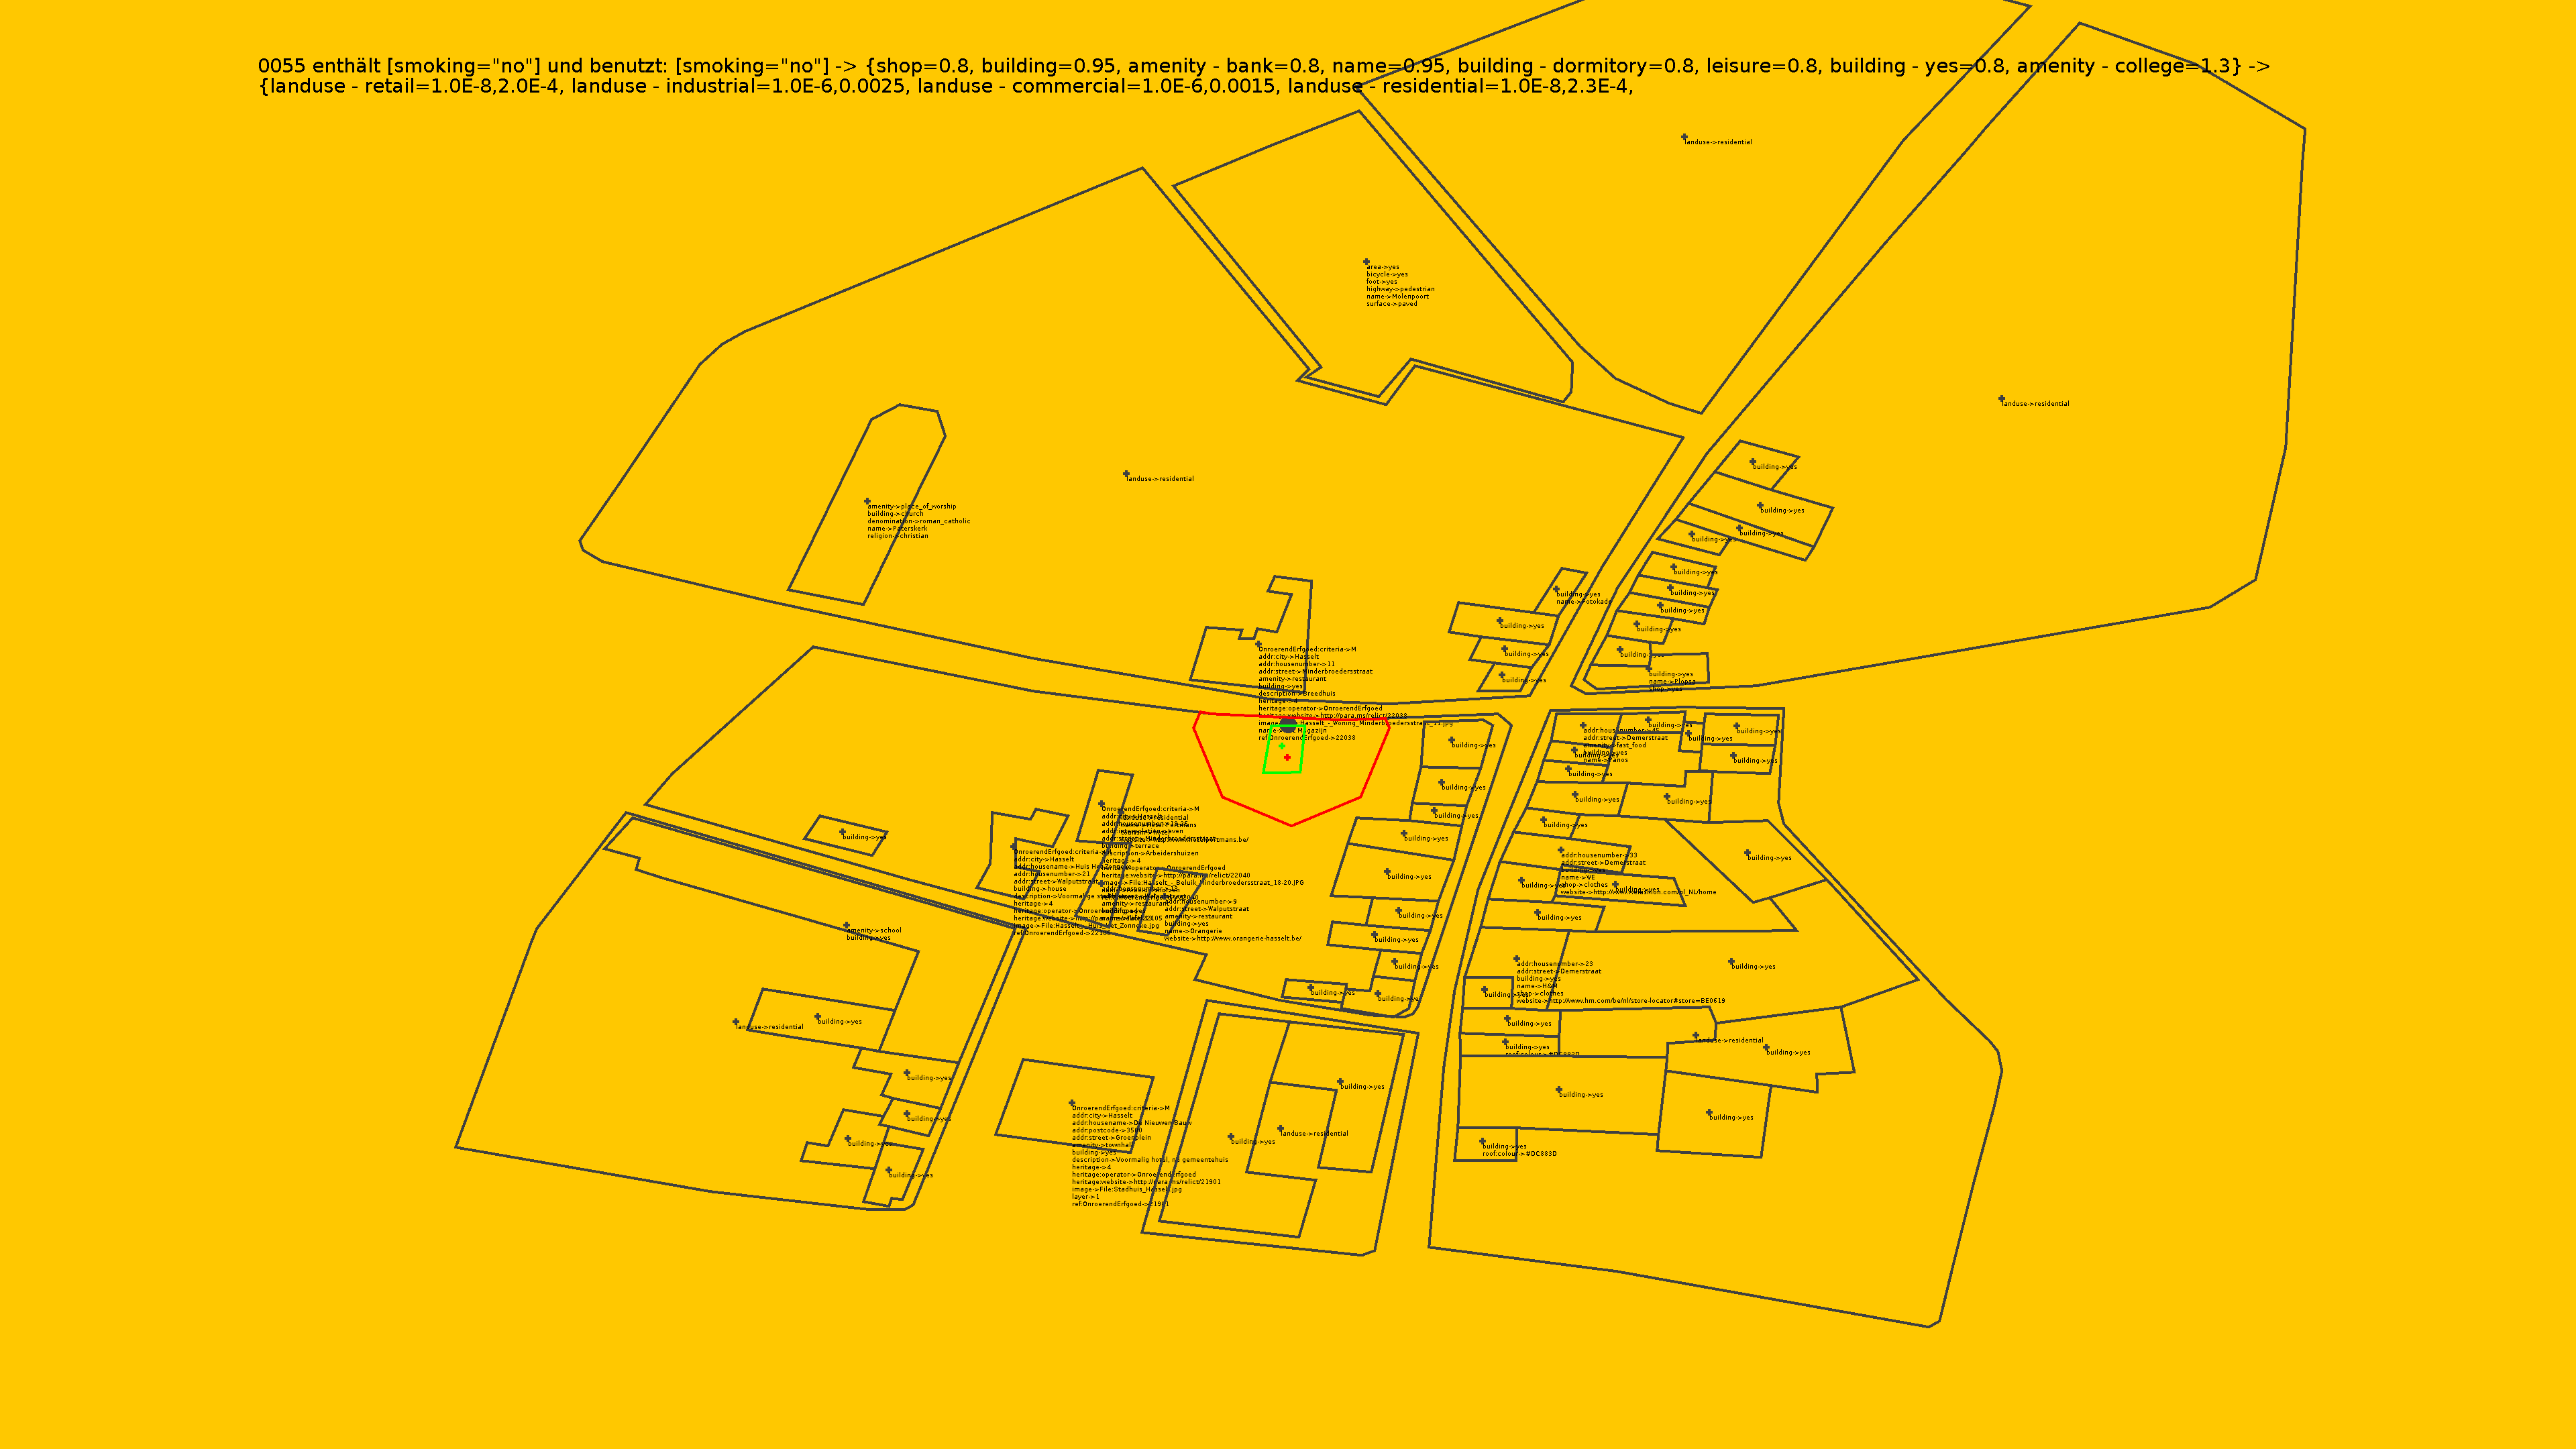
\includegraphics[width=\textwidth]{0055_big.png}}
\end{frame}


\begin{frame}
 \frametitle{Nicht geschafft}
  \Wider{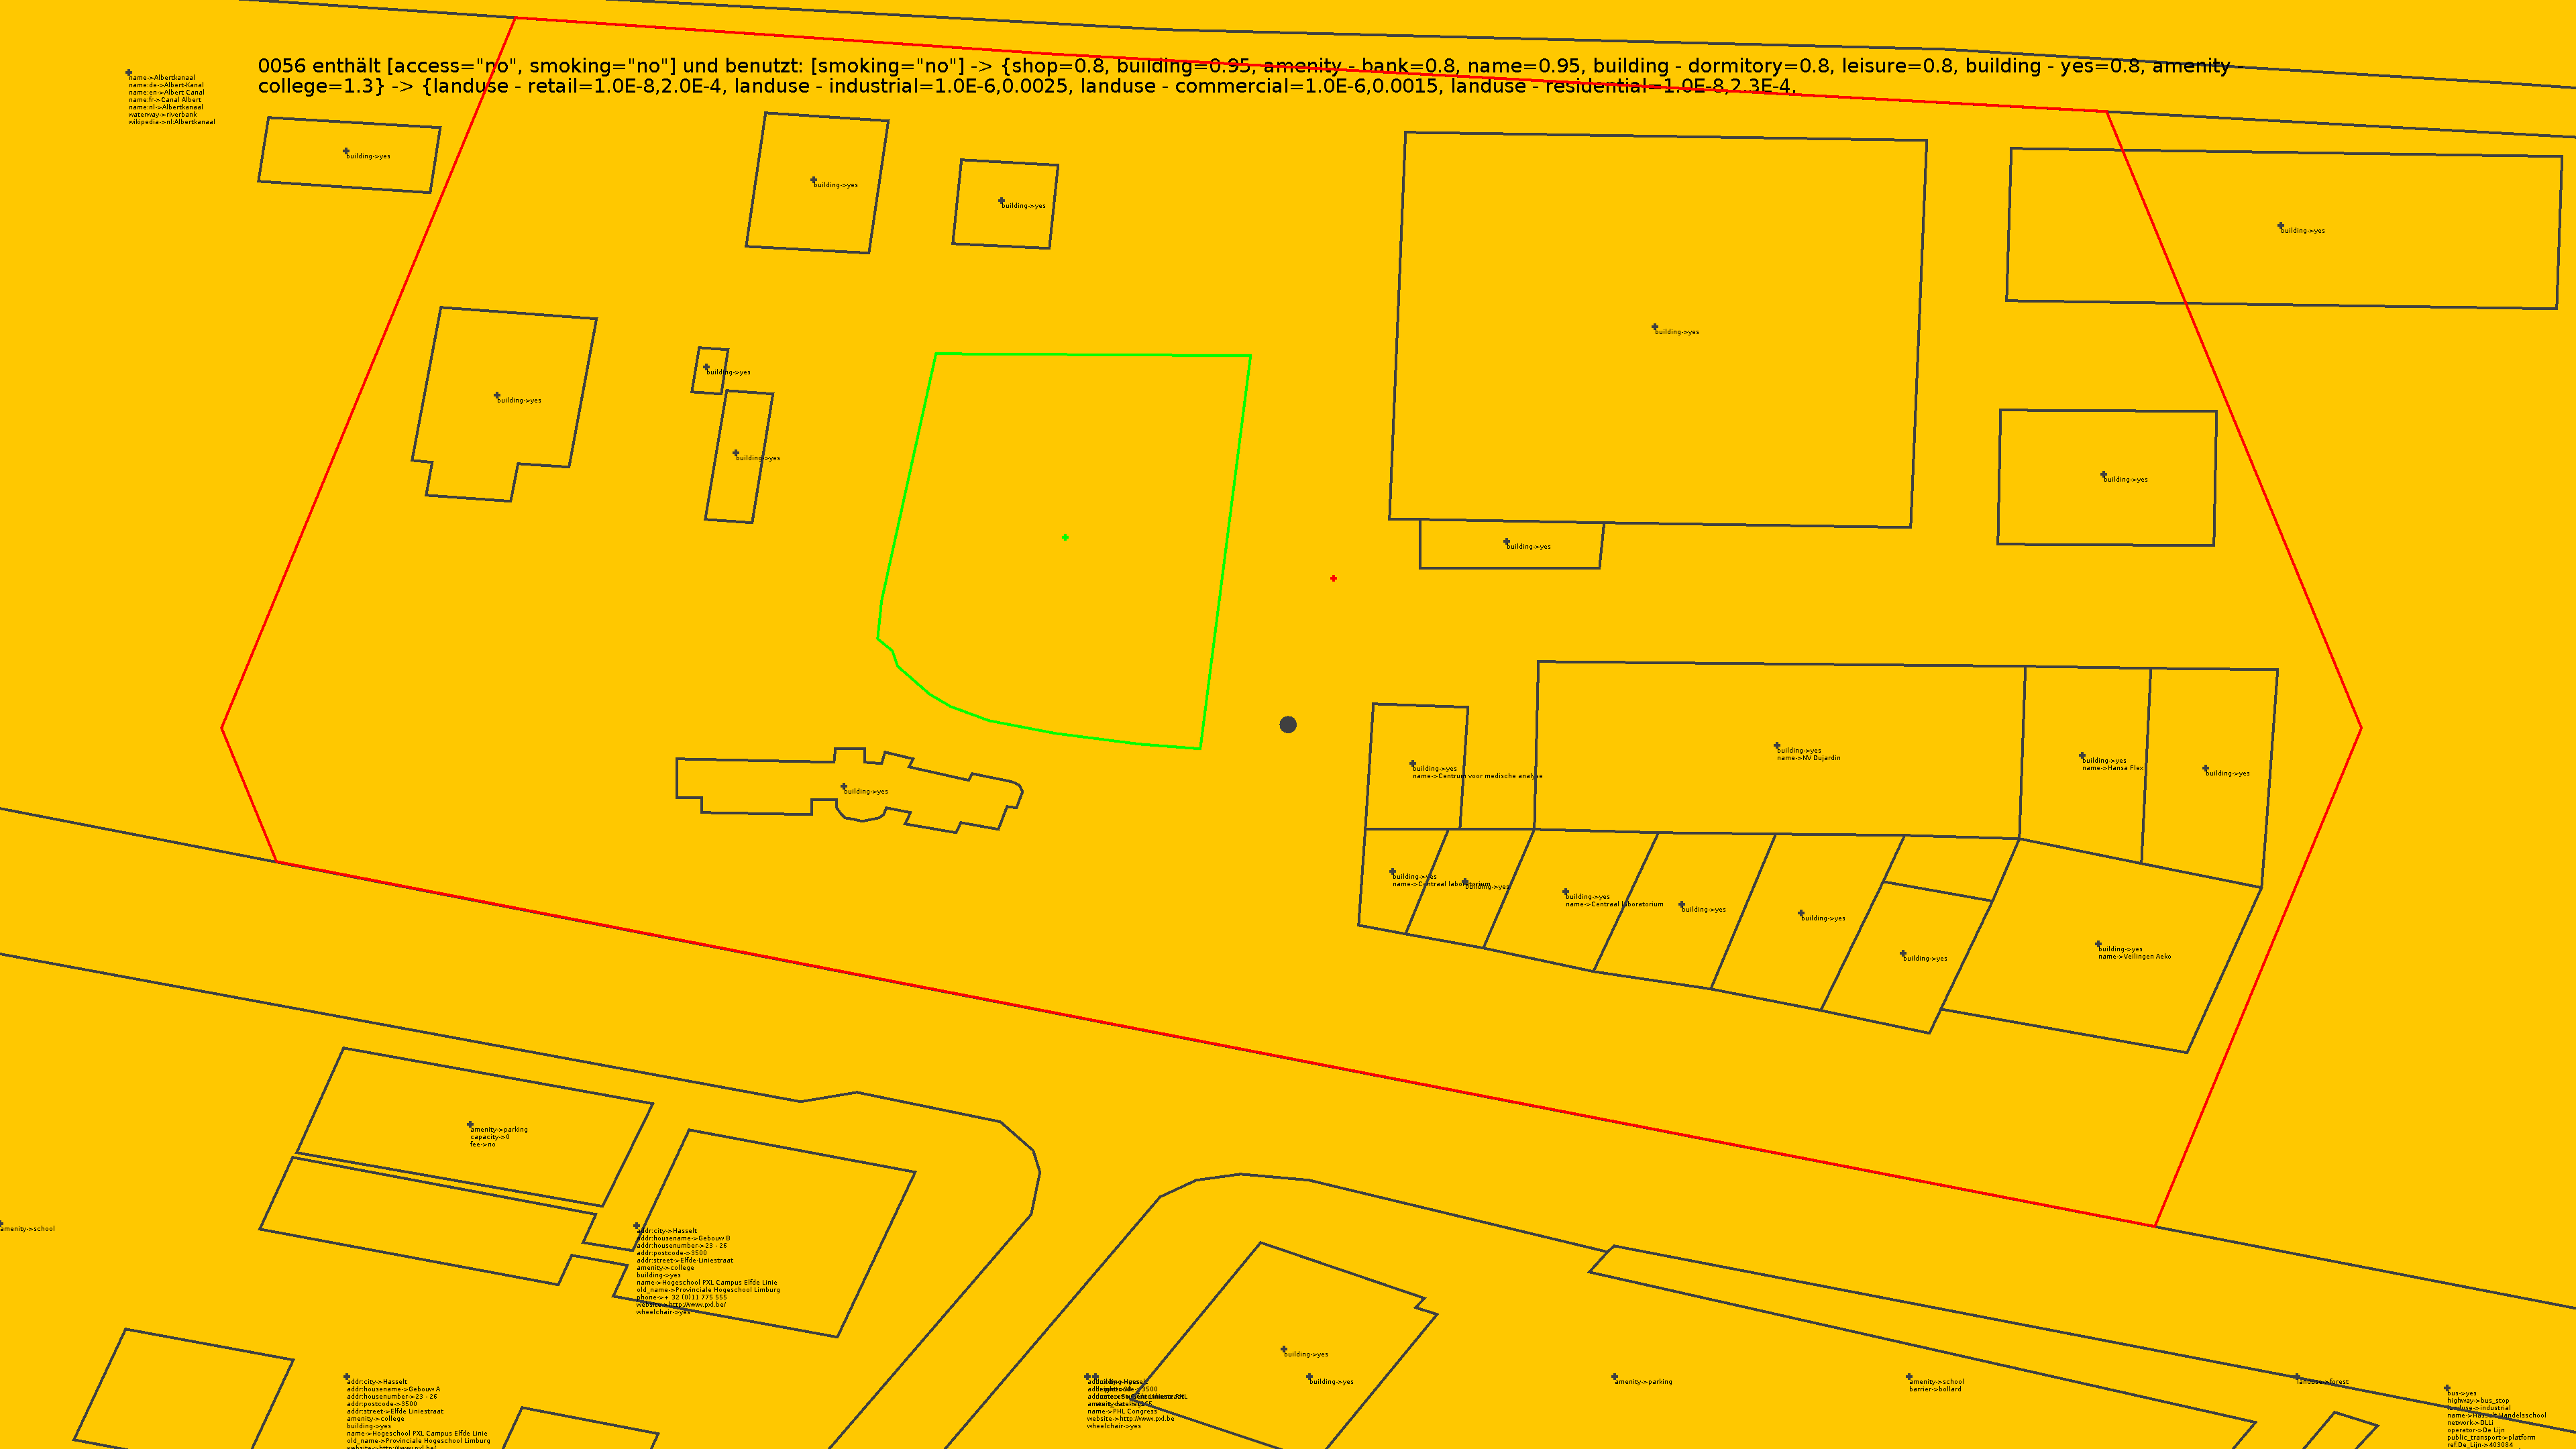
\includegraphics[width=\textwidth]{0056_big.png}}
\end{frame}


\begin{frame}
 \frametitle{Nicht geschafft}
  \Wider{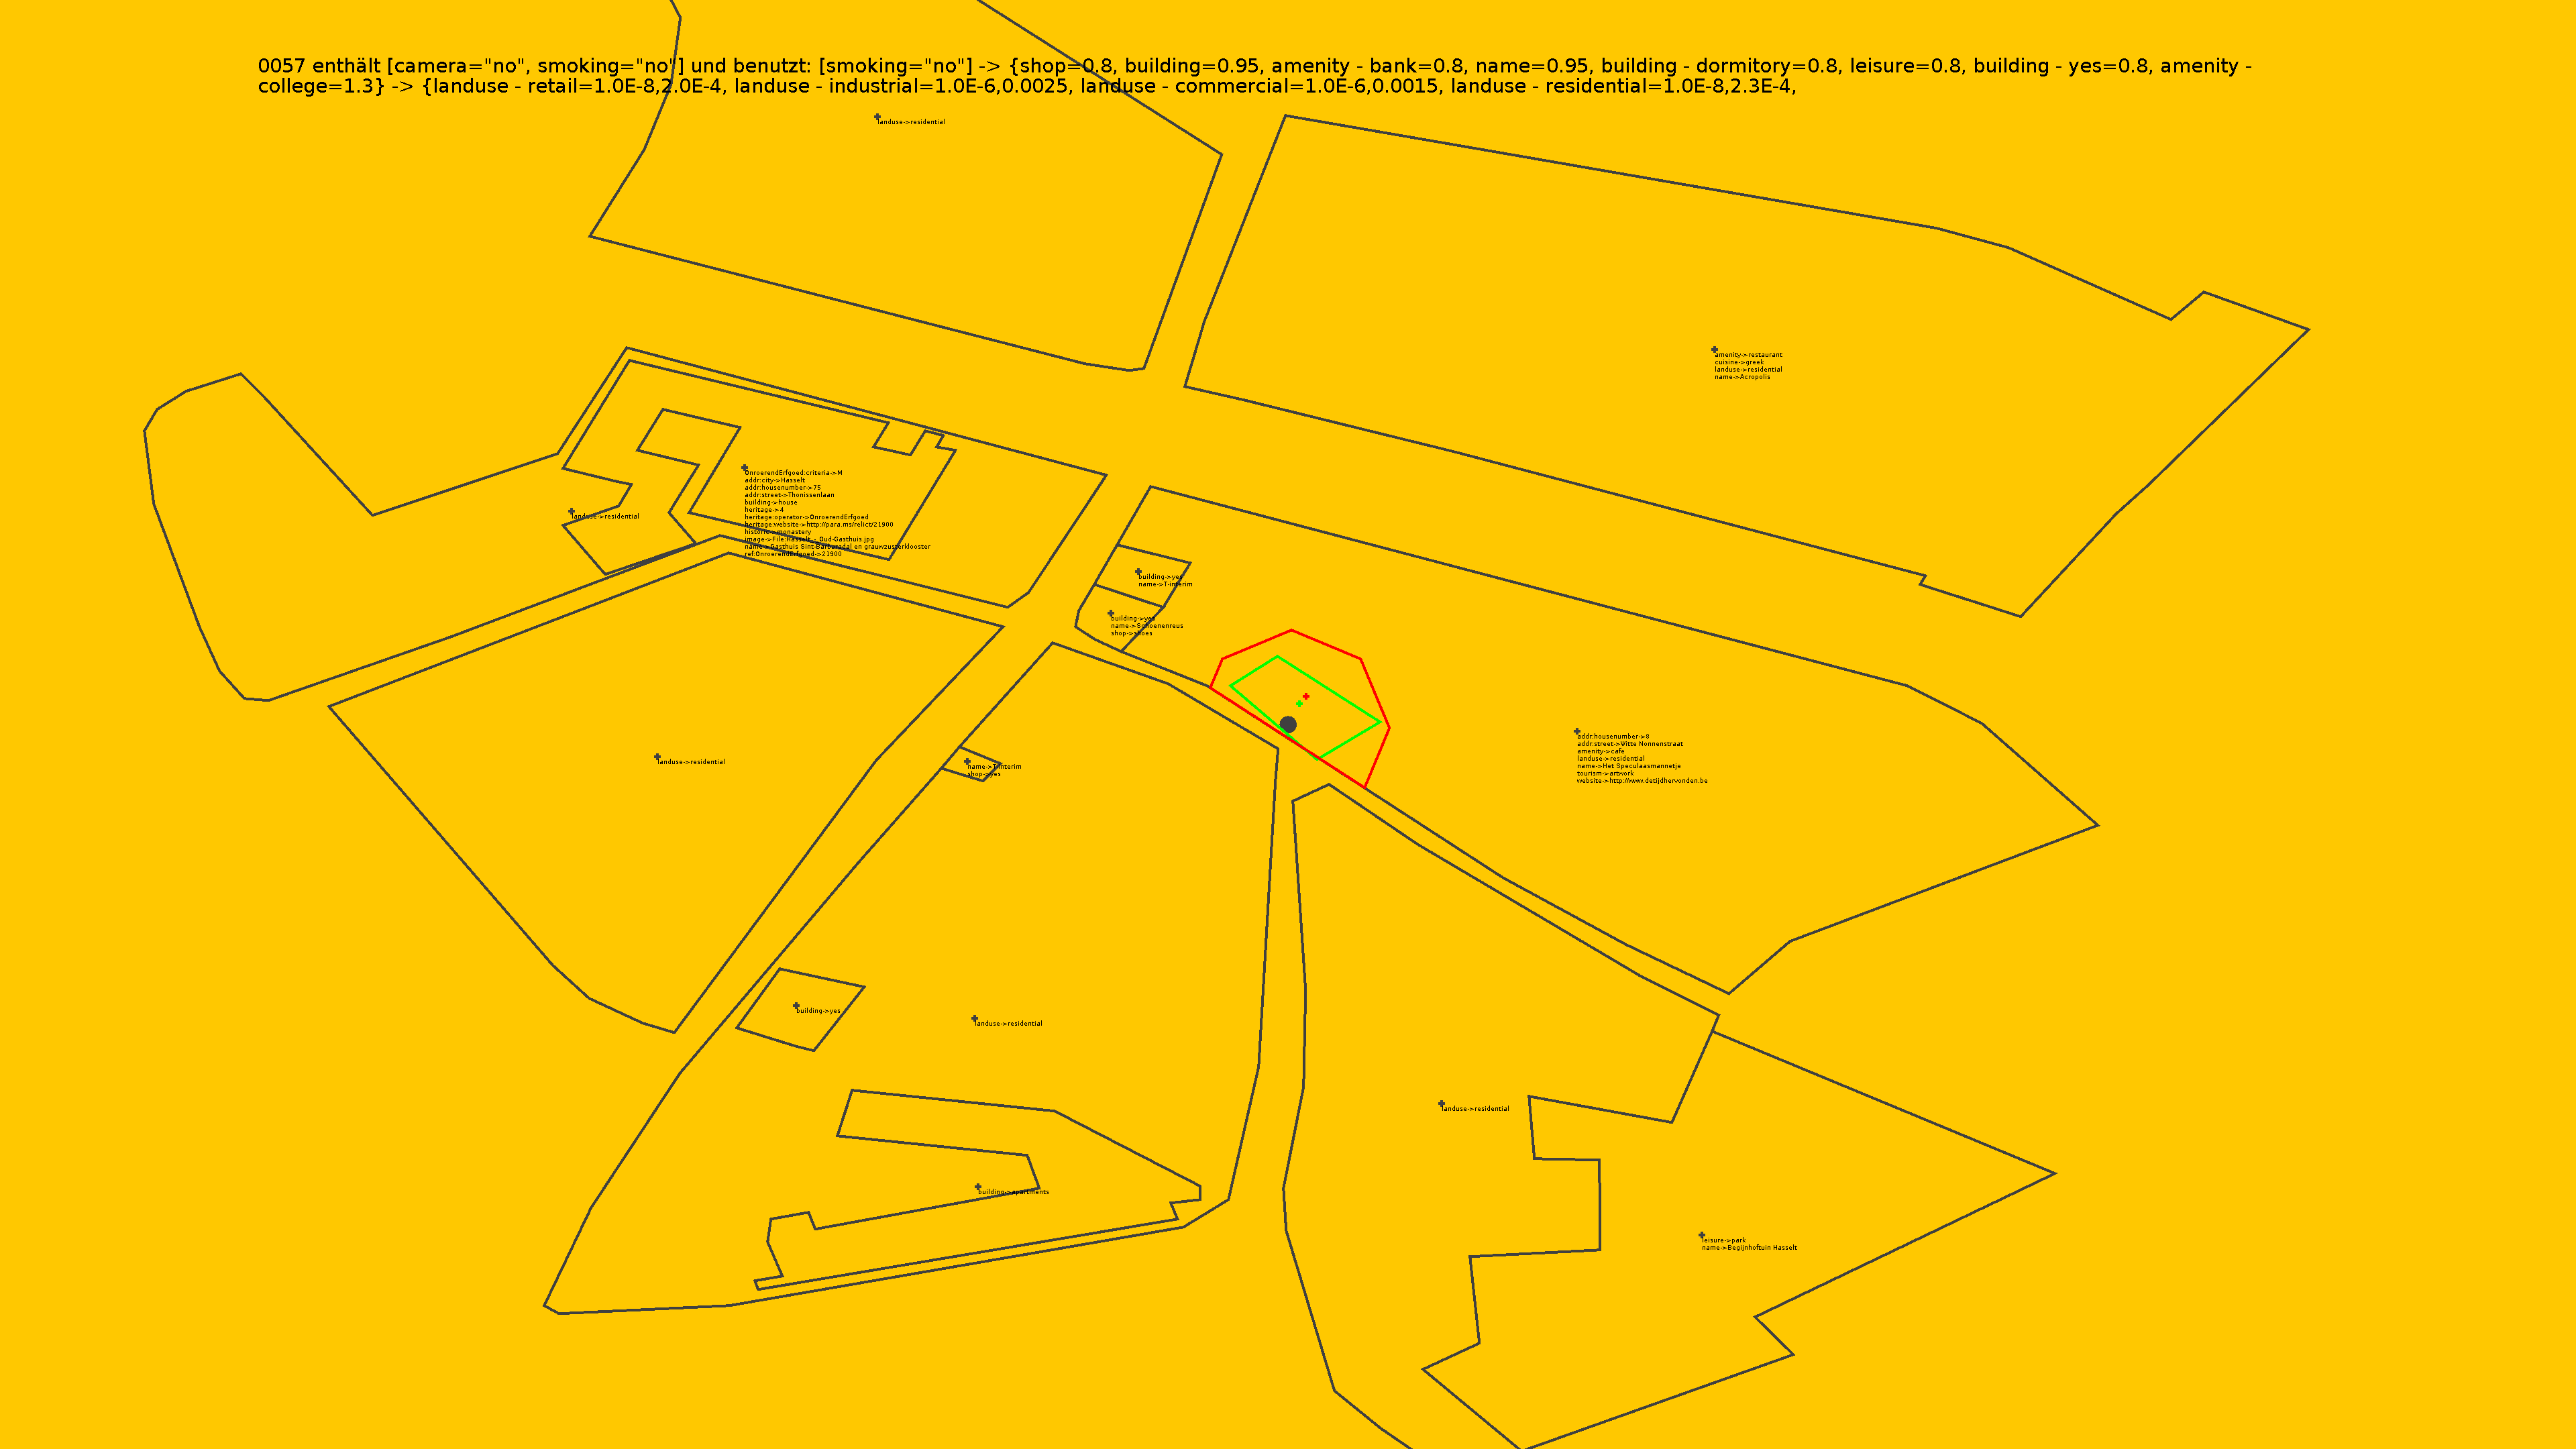
\includegraphics[width=\textwidth]{0057_big.png}}
\end{frame}


\begin{frame}
 \frametitle{Nicht geschafft}
  \Wider{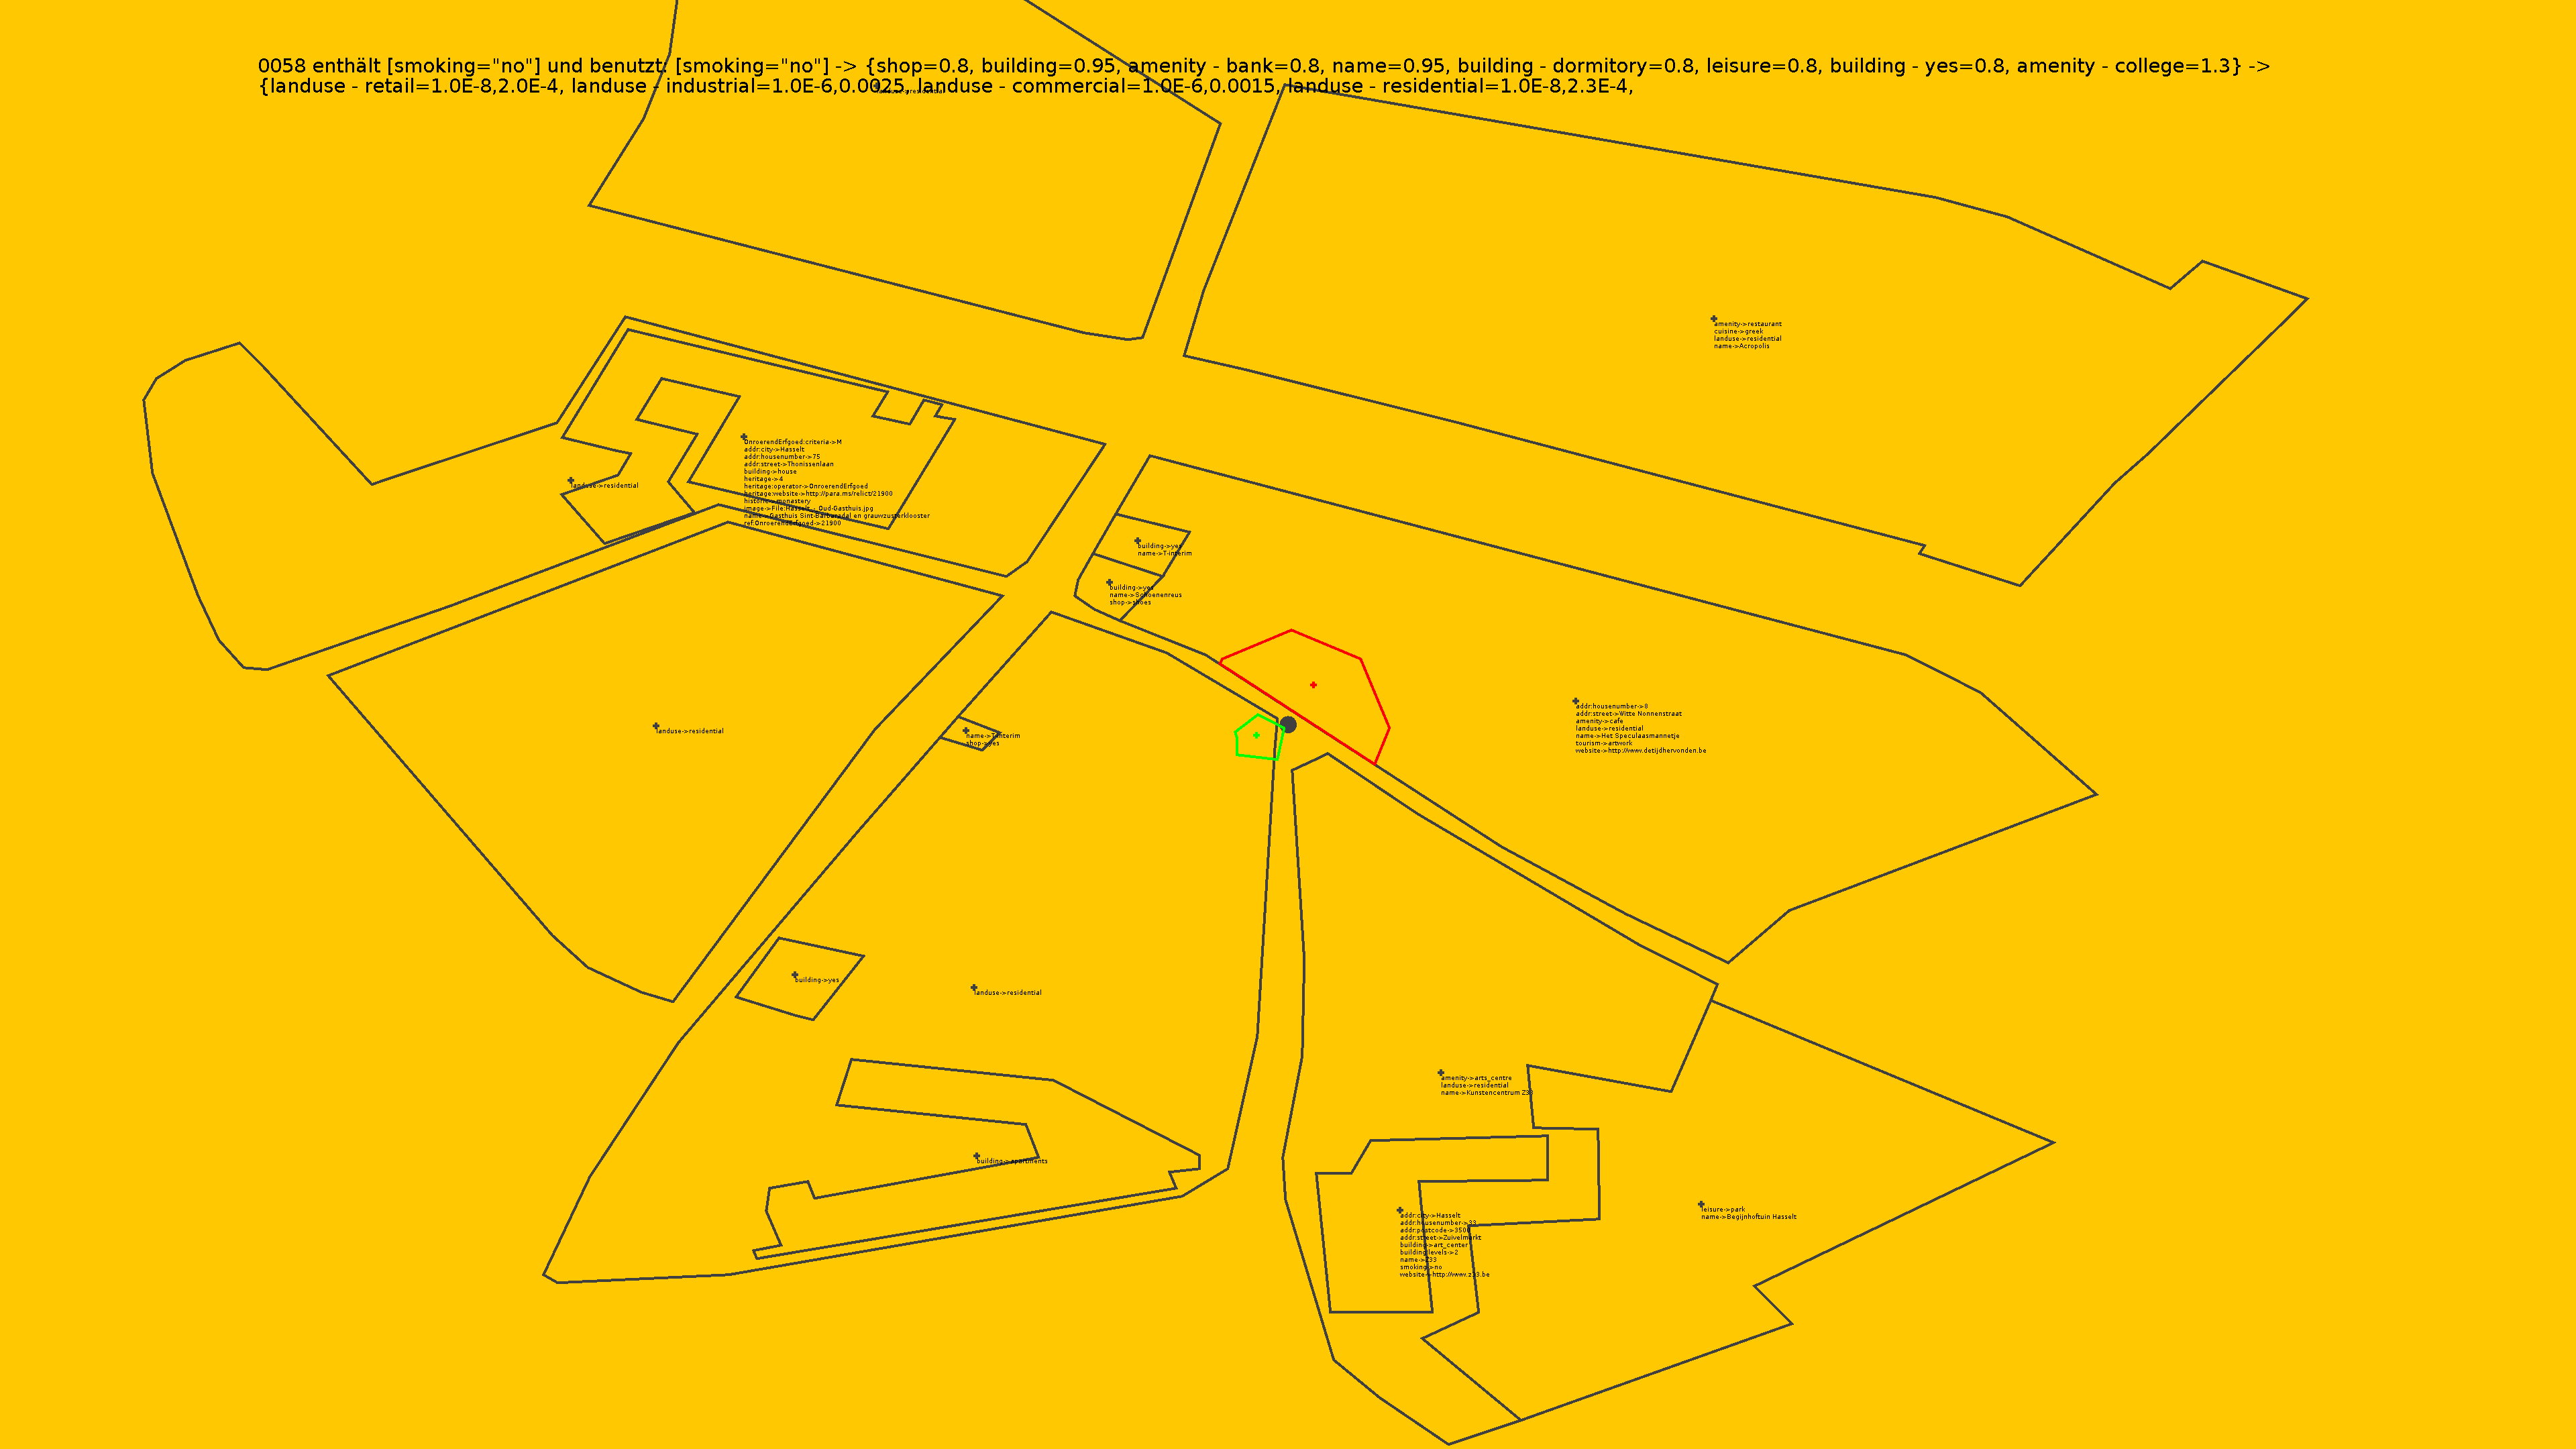
\includegraphics[width=\textwidth]{0058_big.png}}
\end{frame}


\begin{frame}
 \frametitle{Nicht geschafft}
  \Wider{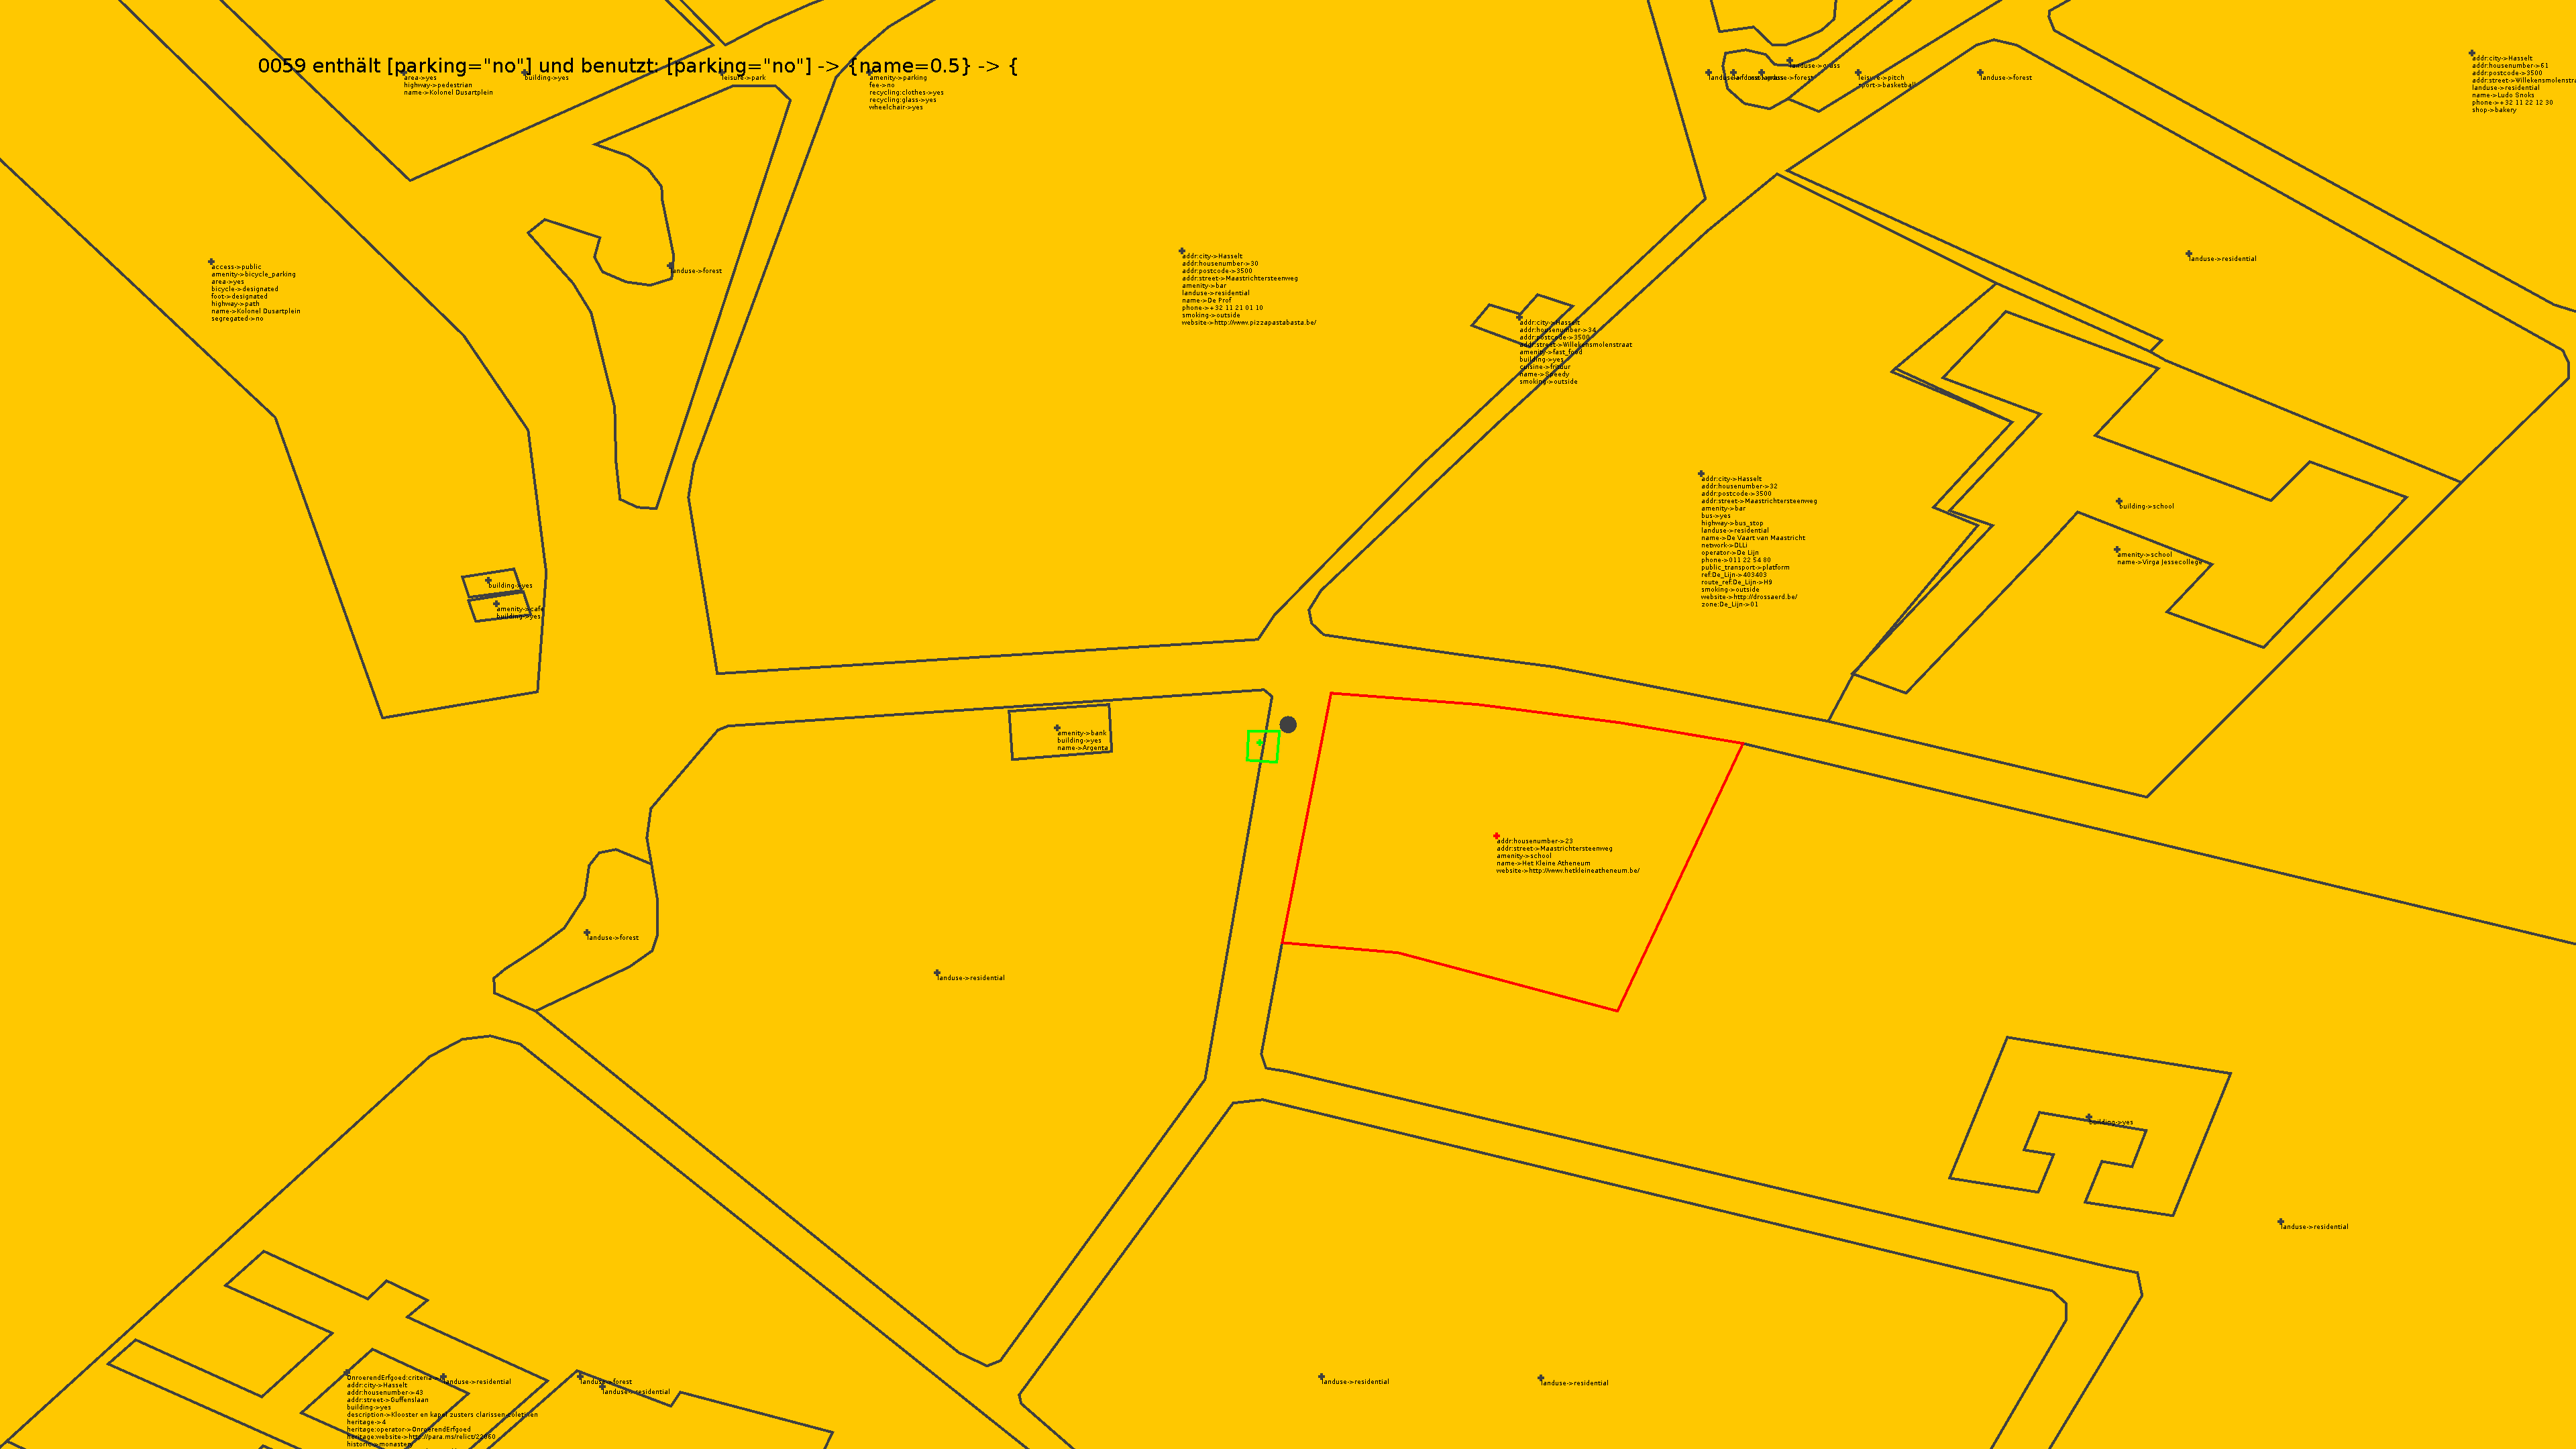
\includegraphics[width=\textwidth]{0059_big.png}}
\end{frame}


\begin{frame}
 \frametitle{Nicht geschafft}
  \Wider{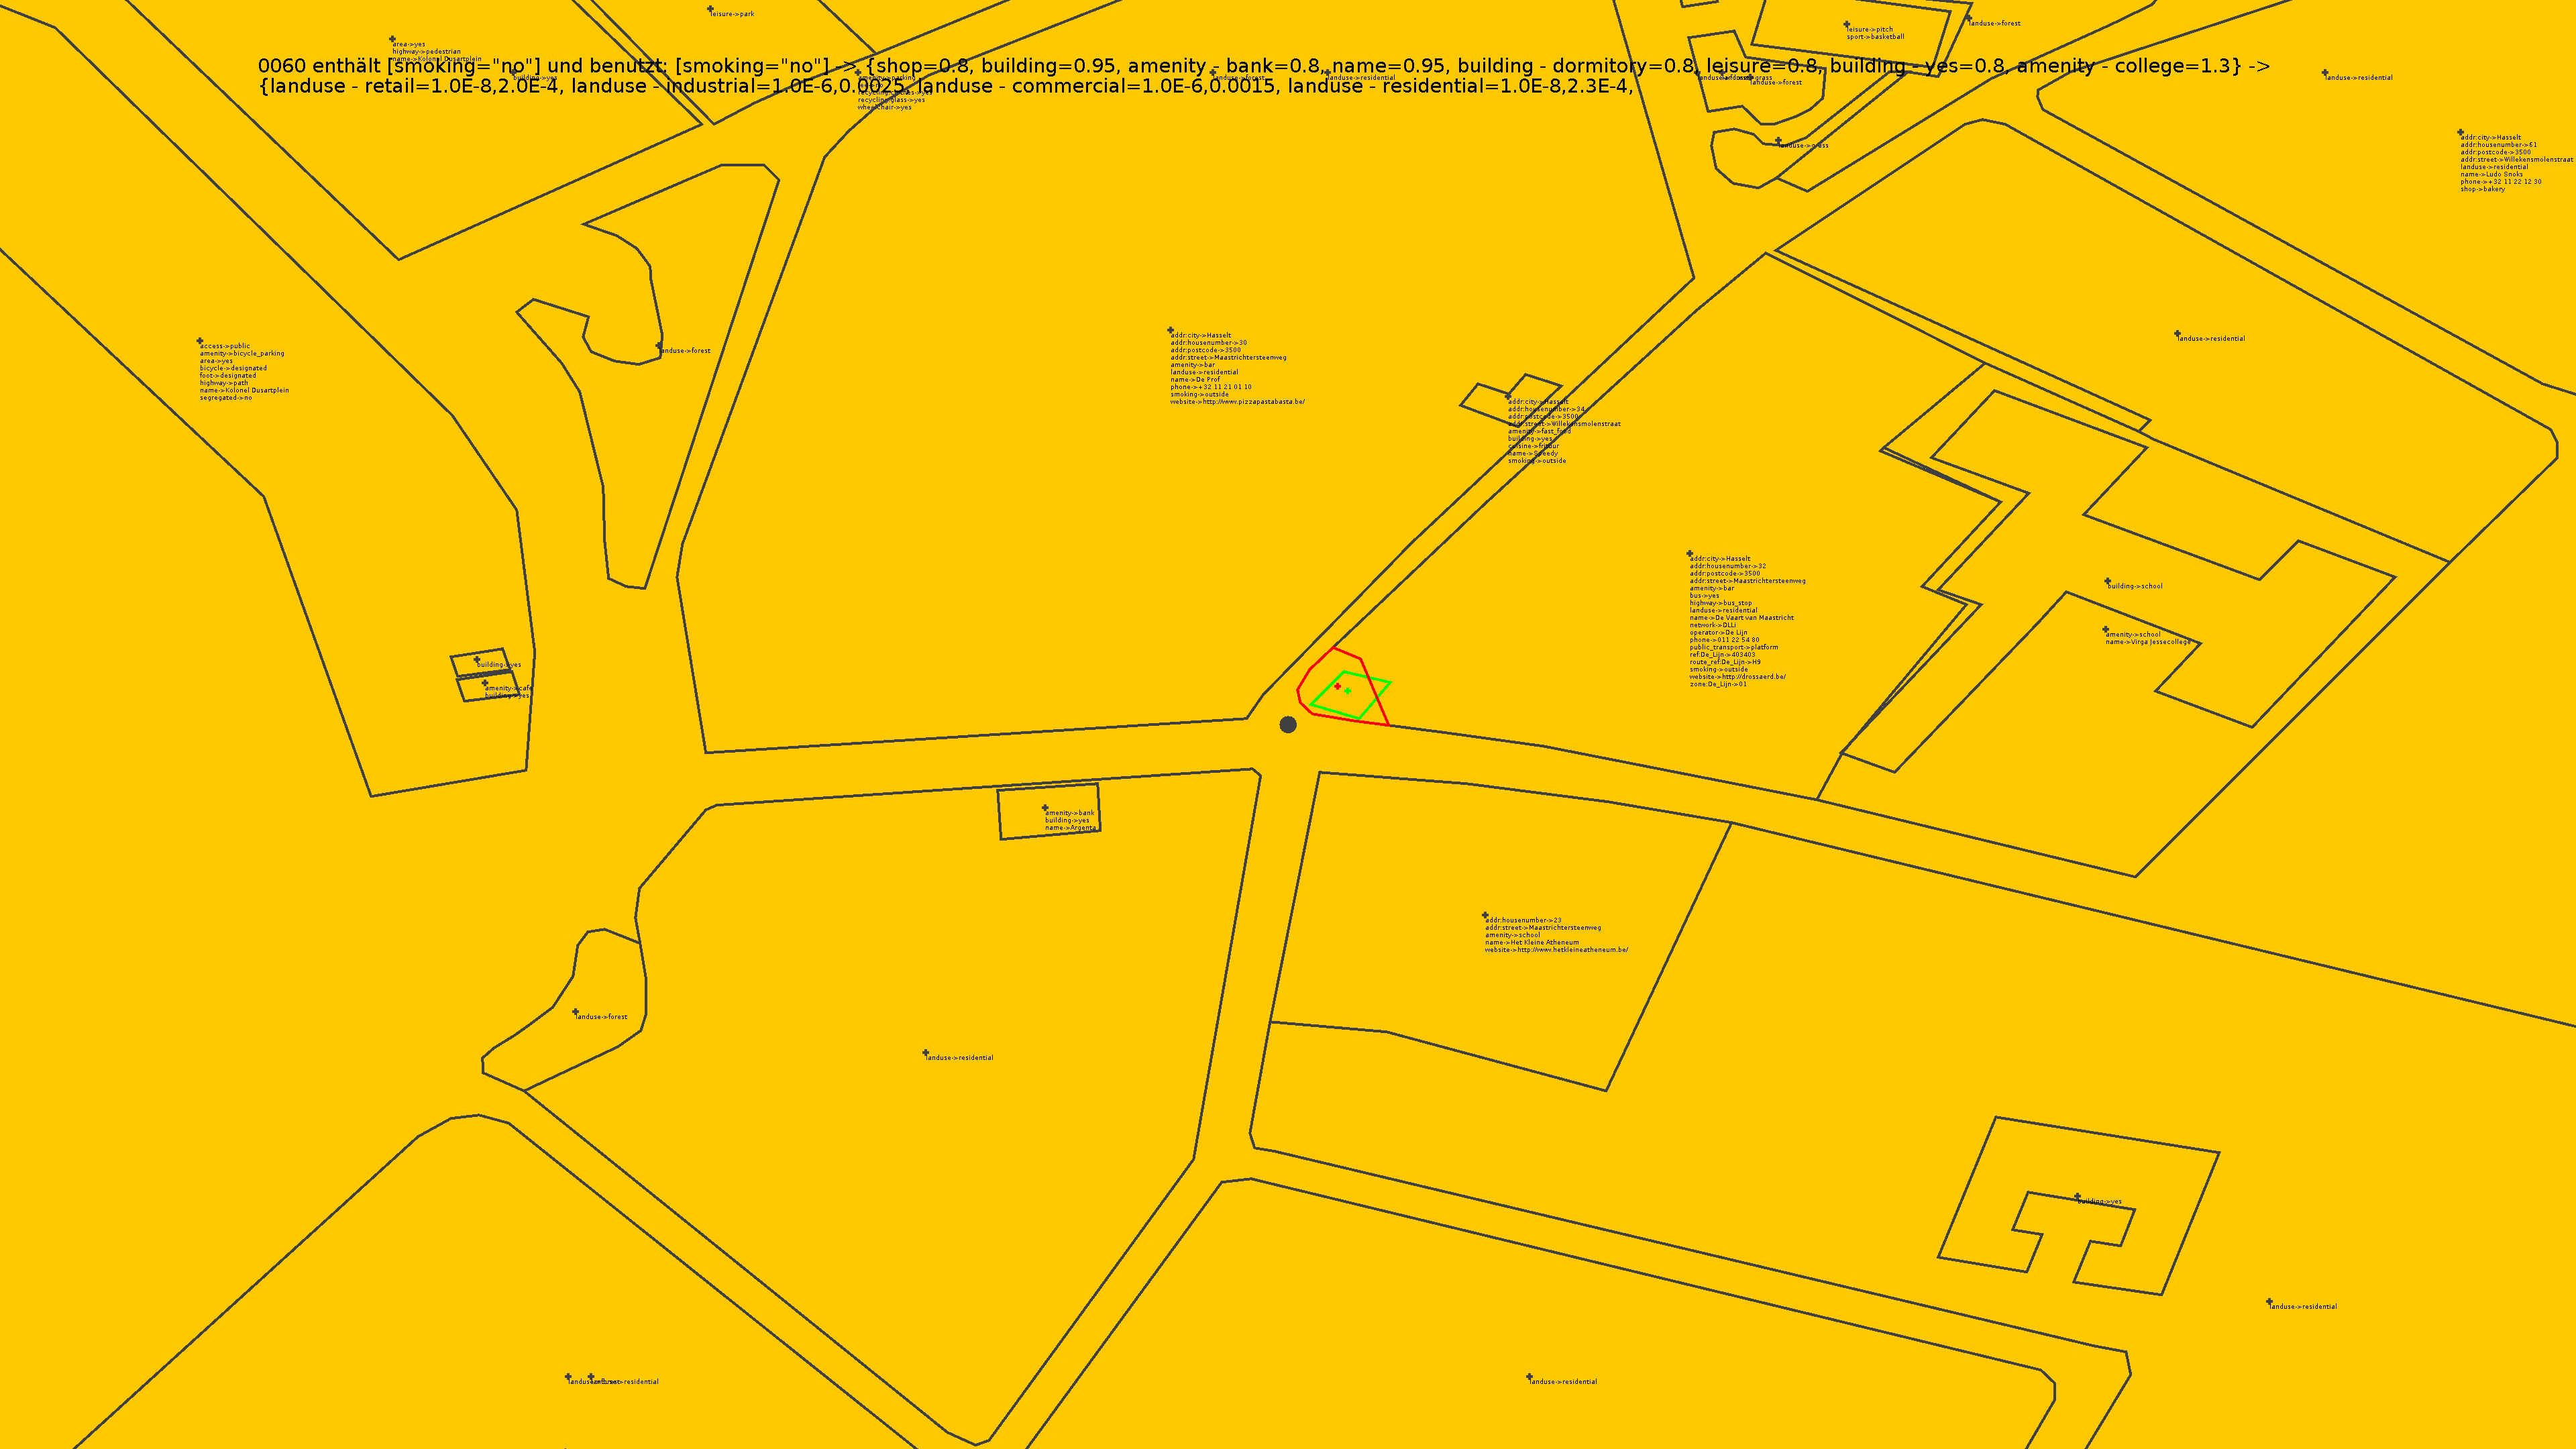
\includegraphics[width=\textwidth]{0060_big.png}}
\end{frame}


\begin{frame}
 \frametitle{Nicht geschafft}
  \Wider{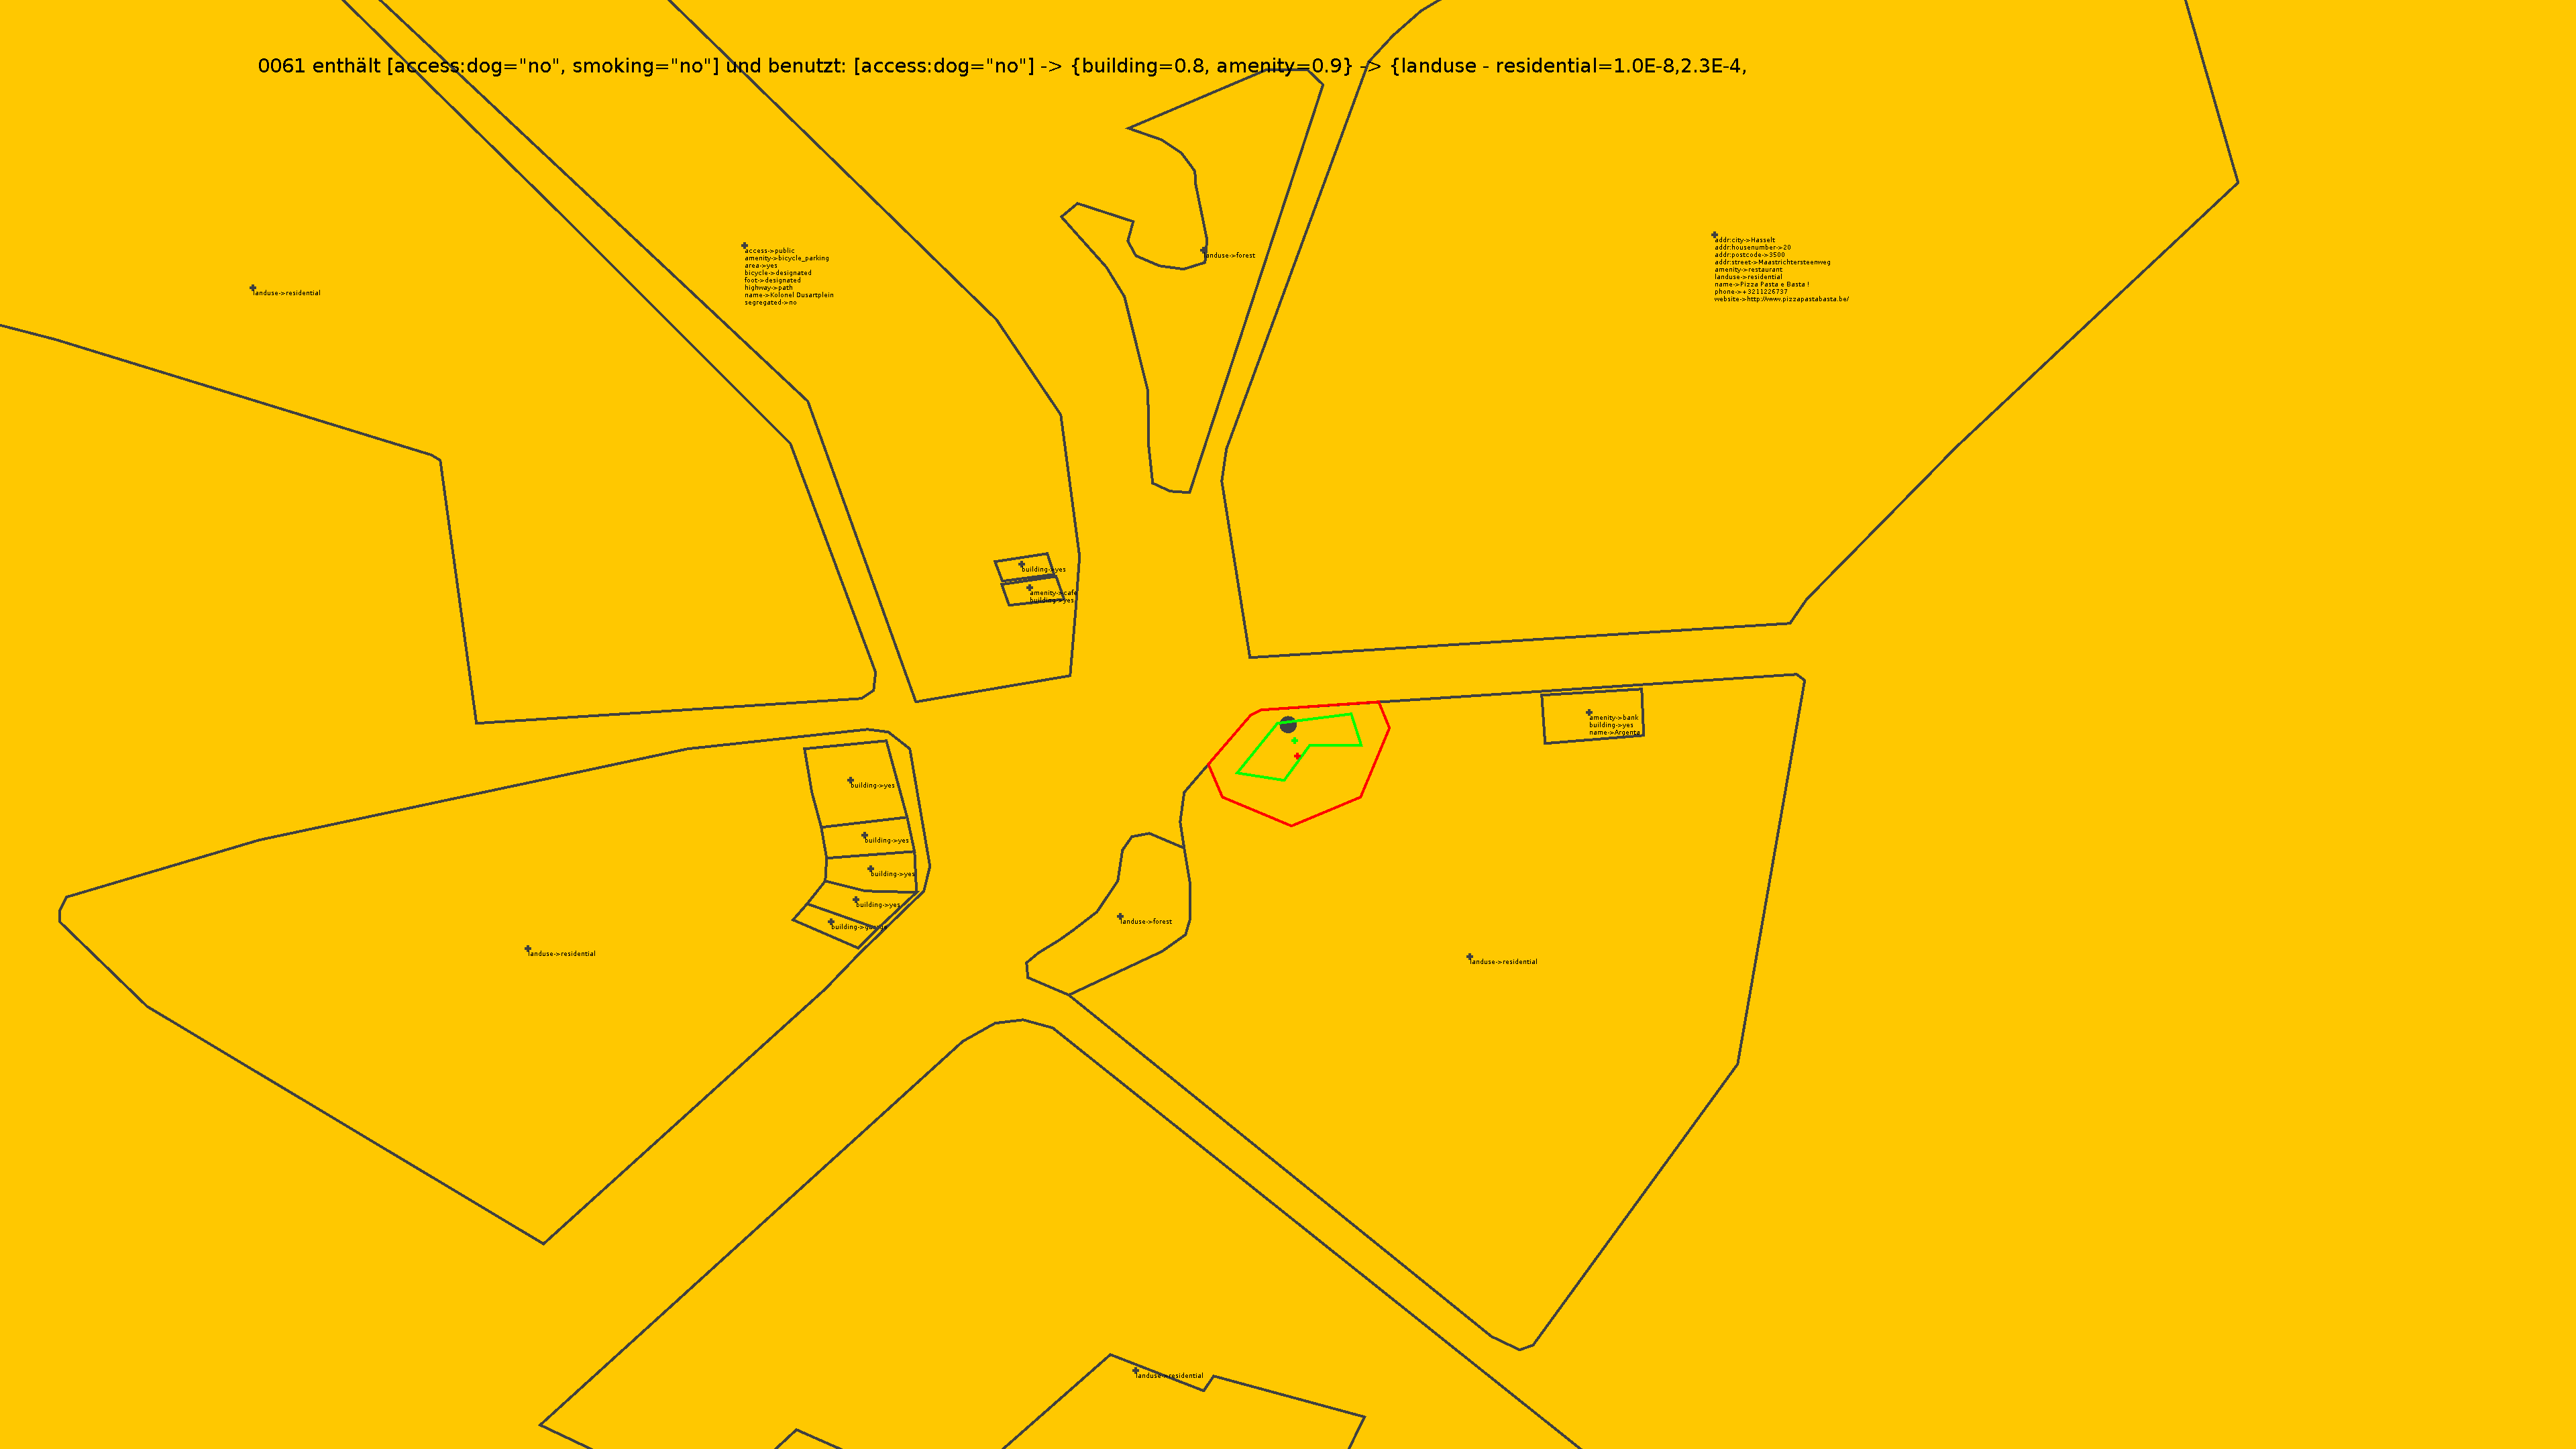
\includegraphics[width=\textwidth]{0061_big.png}}
\end{frame}


\begin{frame}
 \frametitle{Nicht geschafft}
  \Wider{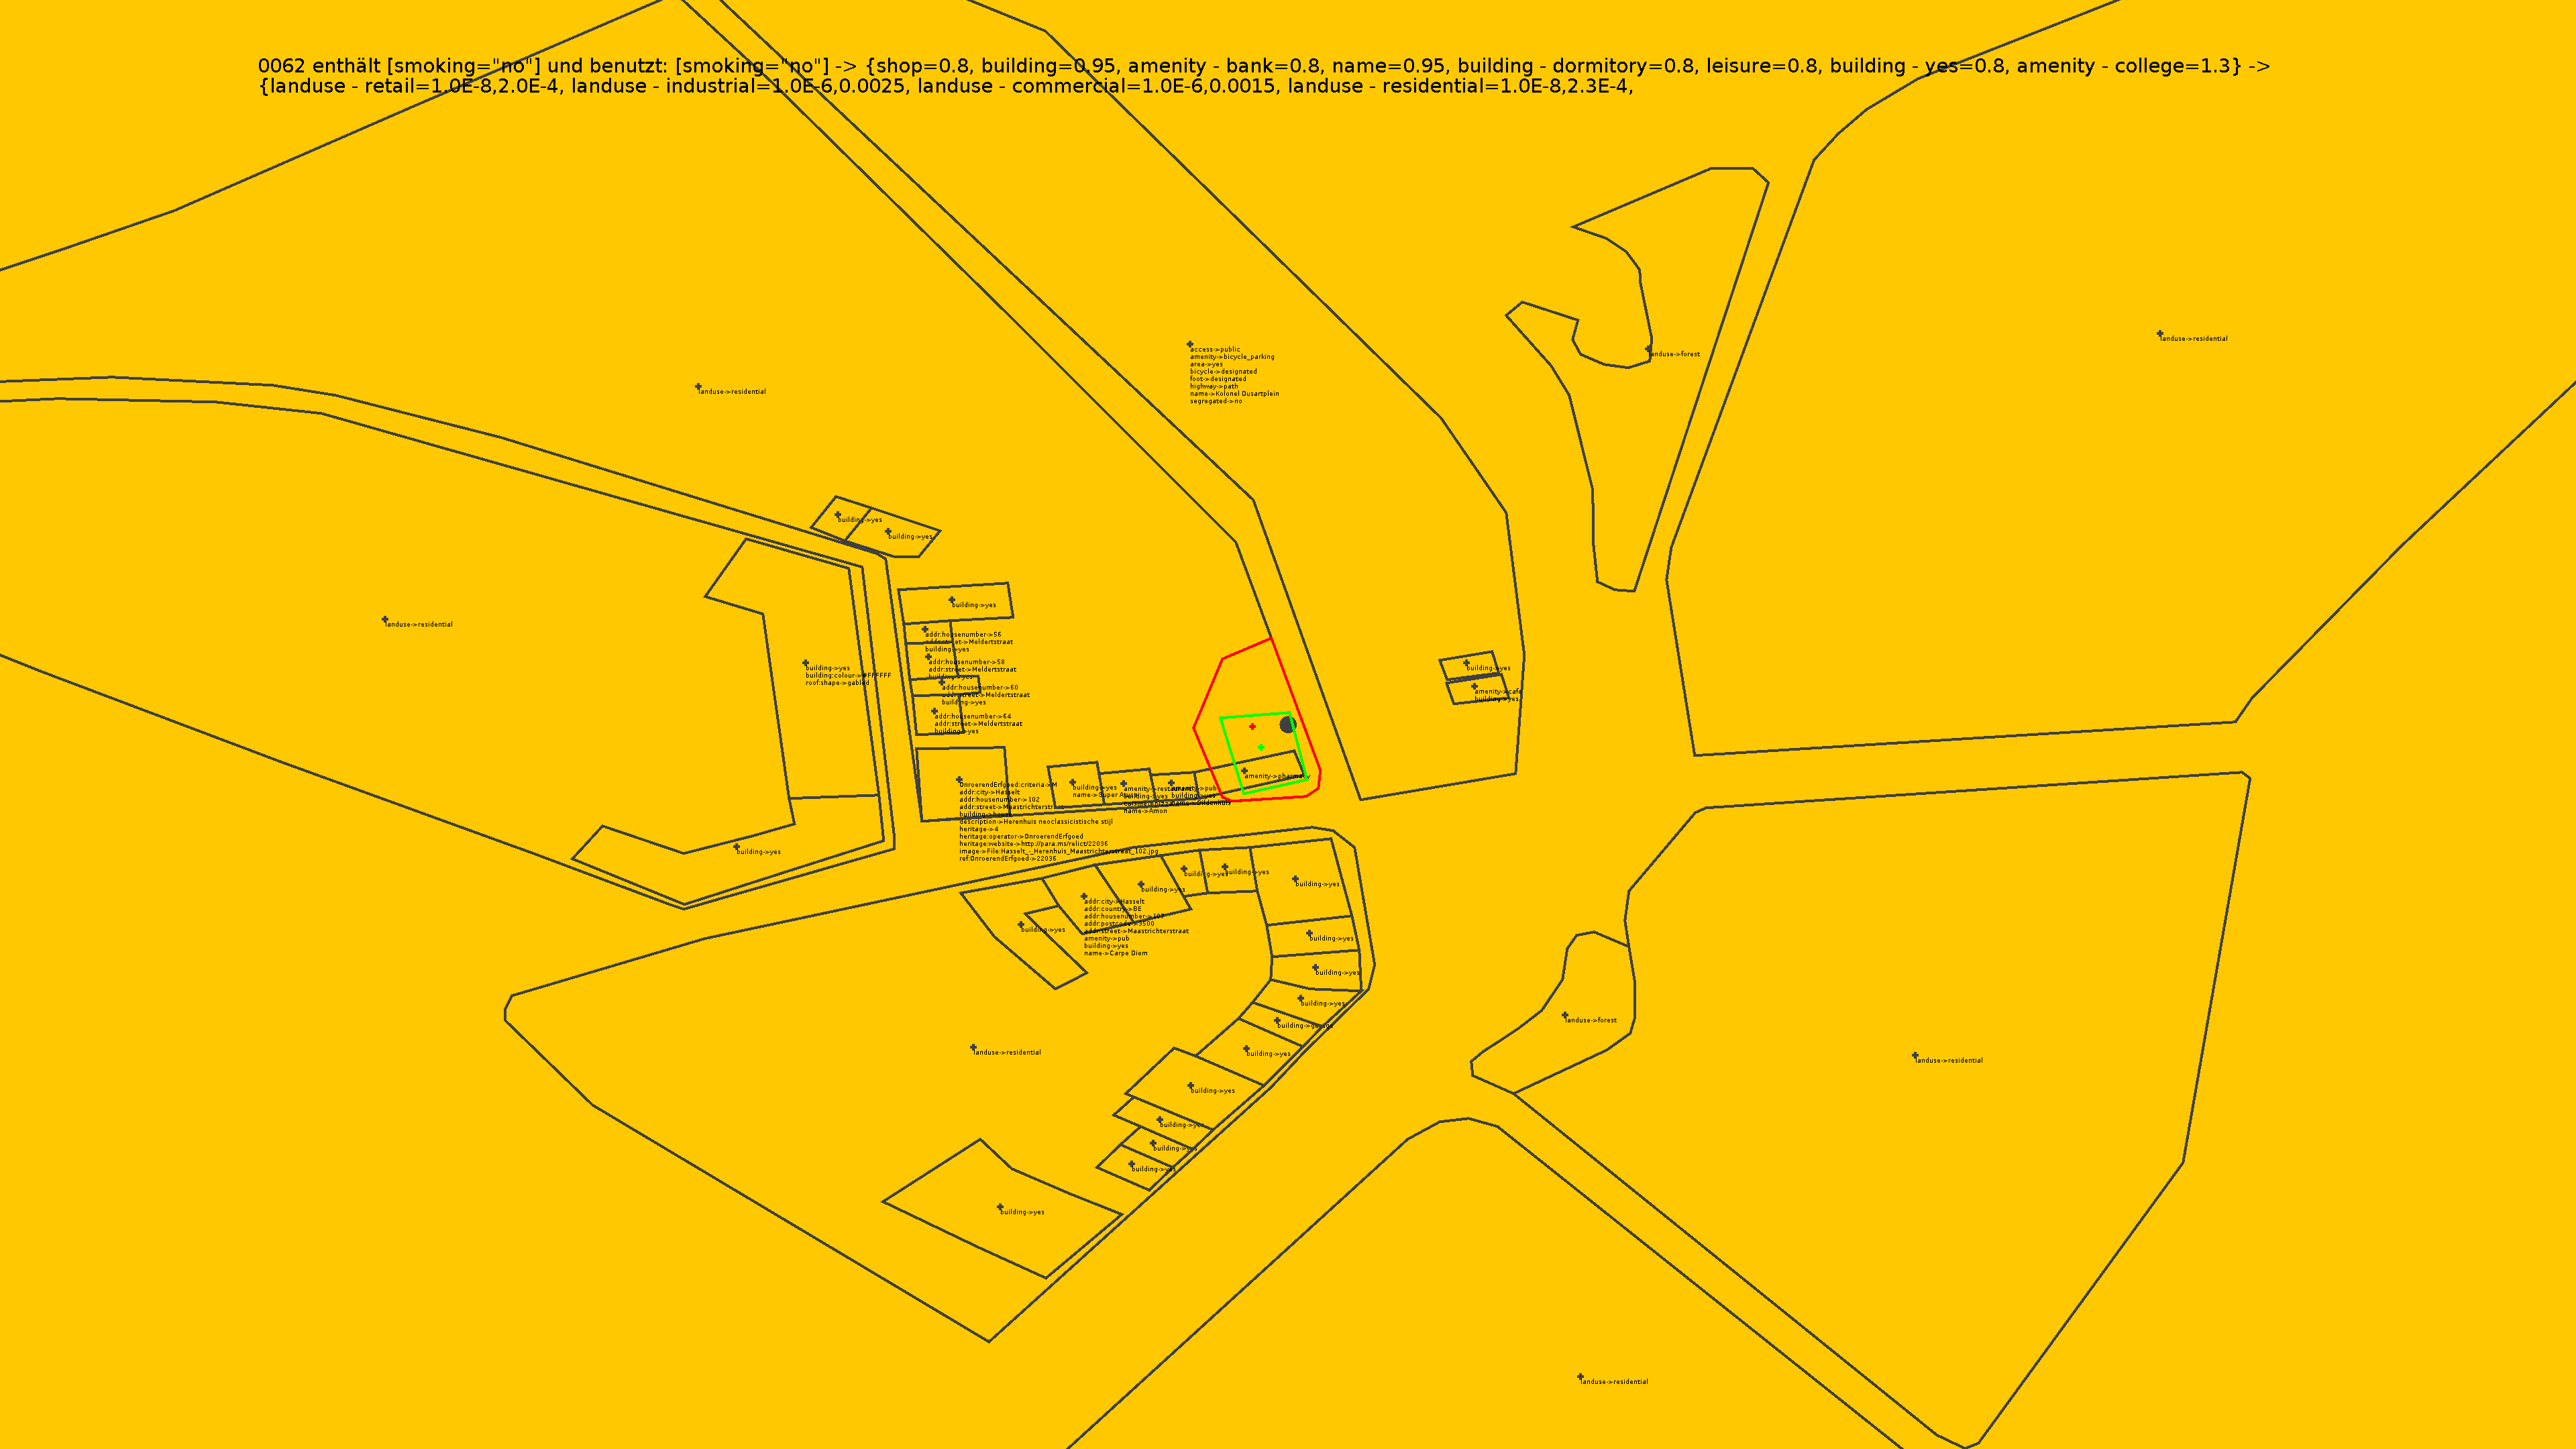
\includegraphics[width=\textwidth]{0062_big.png}}
\end{frame}


\end{document}
